% Created with jtex v.1.0.21
\documentclass{article}
\usepackage{hyperref}
\usepackage{datetime}
\usepackage{graphicx}
\usepackage{natbib}
\bibliographystyle{abbrvnat}

%%%%%%%%%%%%%%%%%%%%%%%%%%%%%%%%%%%%%%%%%%%%%%%%%%
%%%%%%%%%%%%%%%%%%%%  imports  %%%%%%%%%%%%%%%%%%%
\usepackage{booktabs}
\usepackage{framed}
\usepackage{url}
%%%%%%%%%%%%%%%%%%%%%%%%%%%%%%%%%%%%%%%%%%%%%%%%%%


% colors for hyperlinks
\hypersetup{colorlinks=true, allcolors=blue}

\newcommand{\logo}{
  \href{https://curvenote.com}{
\includegraphics[width=2cm]{curvenote.png}}
}

\title{GeospaceLAB-Swarm Guide}

\author{Lei Cai}

\newdate{articleDate}{27}{5}{2026}
\date{\displaydate{articleDate}}

\begin{document}
\maketitle
\begin{center}\logo\end{center}


\section{Getting Started}

\subsection{Overview}

\subsubsection{What is GeospaceLAB?}

Research projects in space physics and space weather are typically based on several kinds of measured and/or modelling data. Processing and combining those data are demanding tasks because they are often provided from different data sources and in different formats.  Even one satellite mission, such as Swarm, may include tens of data products. The diversity of data adds an unnecessary complexity to the data analysis in research projects. It often takes a lot of time for a researcher to collect and manage the data before the data are processed for a further analysis and interpretation. To improve the productivity in data access and analysis, the open-source Python package GeospaceLAB is developed.

GeospaceLAB provides a unified process for data access, management, and visualization that connects the data provider and the space physics researchers. Using the package, researchers can progress their research in a quick manner and focus more on the data interpretation and research results. The package has been applied in the study of Magnetosphere-ionosphere-thermosphere coupling. The package got 29 stars in GitHub and was included in Python in Heliosphysics Community (PyHC) in 2022.

\begin{framed}
\textbf{Resources}\\
\begin{itemize}
\item GeospaceLAB GitHub repository: \href{https://github.com/JouleCai/geospacelab}{click here}
\item GeospaceLAB Documentation: \href{https://geospacelab.readthedocs.io/en/latest/}{click here}
\item GeospaceLAB PyPI package: \href{https://pypi.org/project/geospacelab/}{click here}
\item GeospaceLAB Swarm support documentation: \href{https://geospacelab-swarm.readthedocs.io/en/latest/}{click here}
\item GeospaceLAB Swarm support GitHub repository: \href{https://github.com/JouleCai/geospacelab-swarm}{click here}
\end{itemize}
\end{framed}

\subsubsection{Supported Swarm data products in GeospaceLAB}

As listed in Table~\ref{tab:swarm-products}, GeospaceLAB currently supports 30 data products of Swarm mission. Those data products are selected from the categories of ``Ionosphere/Magnetosphere'', ``Thermosphere'', ``Space Weather'', and ``Magnetic measurements'' in the \href{https://swarmhandbook.earth.esa.int/catalogue/index}{Swarm Product Data Handbook}.

Users can easily access the listed Swarm data products from (1) ESA's \href{https://earth.esa.int/eogateway/missions/swarm/data}{Swarm Dissemination Sever}, (2) \href{https://vires.services/}{Swarm VirES Service\textsuperscript{*}}, and (3) \href{https://vires.services/hapi}{VirES for Swarm - HAPI Server\textsuperscript{*}}. The data access and visualization are tested and verified in GeospaceLAB.

\begin{framed}
\textbf{Note}\\
\textsuperscript{*}: For VirES and VirES HAPI server, only the MAG data is currently supported. The support for other data products is under development and will be released in the future.
\end{framed}

\begin{table}
\centering
\caption[]{Supported Swarm data products in GeospaceLAB}
\label{tab:swarm-products}
\begin{tabular}{p{\dimexpr 0.167\linewidth-2\tabcolsep}p{\dimexpr 0.167\linewidth-2\tabcolsep}p{\dimexpr 0.167\linewidth-2\tabcolsep}p{\dimexpr 0.167\linewidth-2\tabcolsep}p{\dimexpr 0.167\linewidth-2\tabcolsep}p{\dimexpr 0.167\linewidth-2\tabcolsep}}
\toprule
No. & Product & Level & Folder & Description & Status \\
\hline
1 & SW\_AEJxLPL\_2F & 2 & Level2daily & Auroral electrojets line profile -- Line current method (LC) & Tested \\
2 & SW\_AEJxLPS\_2F & 2 & Level2daily & Auroral electrojets line profile -- SECS method & Tested \\
3 & SW\_AEJxPBL\_2F & 2 & Level2daily & Auroral electrojets peaks and boundaries from LC & Tested \\
4 & SW\_AEJxPBS\_2F & 2 & Level2daily & Auroral electrojets peaks and boundaries from SECS & Tested \\
5 & SW\_AOBxFAC\_2F & 2 & Level2daily & Auroral oval boundaries derived from FAC & Tested \\
6 & SW\_DNSxACC\_2\_ & 2 & Level2daily & Thermospheric~density derived from ACC + POD & Tested \\
7 & SW\_DNSxPOD\_2\_ & 2 & Level2daily & Thermospheric~density derived from POD & Tested \\
8 & SW\_EFIx\_LP\_1B & 1 & Level1b & Electric field instrument (EFI) Langmuir probe (LP) measurements at 2 Hz & Tested \\
9 & SW\_EFIx\_LP\_FP & Advanced & Advanced/Plasma\_Data & EFI faceplate (FP) plasma density at 16 Hz & Tested \\
10 & SW\_EFIx\_LP\_HM & Advanced & Advanced/Plasma\_Data & EFI LP extended at 2 Hz & Tested \\
11 & SW\_EFIx\_TCT02 & Advanced & Advanced/Plasma\_Data & Extended dataset of EFI TII cross-track ion flow measurements at 2 Hz & Tested \\
12 & SW\_EFIx\_TCT16 & Advanced & Advanced/Plasma\_Data & Extended dataset of EFI TII cross-track ion flow measurements at 16 Hz & Tested \\
13 & SW\_EFIxIDM\_2\_ & Advanced & Advanced/Plasma\_Data & EFI LP ion drift and effective mass & Tested \\
14 & SW\_EFIxLPI\_1B & 1b & Level1b & EFI LP measurements at 1 Hz & Tested \\
15 & SW\_EFIxTIE\_2\_ & 2 & Level2daily & Estimated ion temperatures along Swarm satellite orbits & Tested \\
16 & SW\_EFIxTMS\_2F & 2 & Level2daily & Dayside equatorial electric field & Tested \\
17 & SW\_FAC\_LLS\_2F & 2 & Level2daily & Field-aligned currents (dual-satellite A-C) least-squres & Tested \\
18 & SW\_FAC\_TMS\_2F & 2 & Level2daily & Field-aligned currents (dual-satellite A-C) & Tested \\
19 & SW\_FACxTMS\_2F & 2 & Level2daily & Field-aligned currents (single satellite) & Tested \\
20 & SW\_IBIxTMS\_2F & 2 & Level2daily & Ionospheric bubble index & Tested \\
21 & SW\_IPDxIRR\_2F & 2 & Level2daily & Ionospheric Plasma Irregularities~characterised~by Swarm (IPIR) & Tested \\
22 & SW\_MAGx\_HR\_1B & 1b & Level1b & Magnetic field (50 Hz) from VFM & Tested \\
23 & SW\_MAGx\_LR\_1B & 1b & Level1b & Magnetic field (1 Hz) from VFM and ASM & Tested \\
24 & SW\_MITx\_LP\_2F & 2 & Level2daily & Midlatitude ionospheric trough~boundries~and~minma~drived~from LP & Tested \\
25 & SW\_MITxTEC\_2F & 2 & Level2daily & Midlatitude ionospheric trough~boundries~and~minma~drived~from TEC & Tested \\
26 & SW\_NIX\_TMS\_2F & 2 & Level2daily & NIX & Tested \\
27 & SW\_PPIxFAC\_2F & 2 & Level2daily & Equatorward boundary of SSFACs and the associated midnight PP index & Tested \\
28 & SW\_TECxTMS\_2F & 2 & Level2daily & Ionospheric total electron content & Tested \\
29 & SW\_TIX\_TMS\_2F & 2 & Level2daily & TIX & Tested \\
30 & SW\_WHIxEVT\_2\_ & 2 & Level2daily & Whistler events from ASM BM 250 Hz data & Tested \\
\bottomrule
\end{tabular}
\end{table}

\subsection{Installation}

\subsubsection{Python environment and IDEs}

The Python distribution \textbf{Anaconda} is recommended. To install \textbf{Anaconda}, see \href{https://www.anaconda.com/docs/getting-started/anaconda/install/overview}{Installing Anaconda Distribution}. After installation, a \textbf{conda} virtual environment can be created by, e.g.,

\begin{verbatim}
conda create - -name YOUR_ENV_NAME python=3.12 cython spyder
\end{verbatim}

After creating the virtual environment, one needs to activate it:

\begin{verbatim}
conda activate YOUR_ENV_NAME
\end{verbatim}

\paragraph{Python IDEs}

Popular Python IDEs include \textbf{Spyder}, \textbf{PyCharm}, and \textbf{VS Code}.

\subsubsection{Install GeospaceLAB}

Install GeospaceLAB via PyPI:

\begin{verbatim}
pip install geospacelab
\end{verbatim}

To upgrade GeospaceLAB:

\begin{verbatim}
pip install -U geospacelab
\end{verbatim}

\paragraph{Dependencies}

Most of the dependencies are installed when the package is installed. A few packages can be installed manually.

For example, the \textbf{Cartopy} package is useful for processing and mapping geospatial data. To install \textbf{Cartopy}, see \href{https://cartopy.readthedocs.io/stable/installing.html}{Installing Cartopy}.

Another useful package is \textbf{ApexPy}, which provides a Python interface to the Apex coordinate system. To install \textbf{ApexPy}, see \href{https://apexpy.readthedocs.io/en/latest/installation.html}{Installing ApexPy}.

\begin{framed}
\textbf{Note}\\
To use the VirES and HAPI services, install the \texttt{viresclient}:

\begin{verbatim}
pip install viresclient
\end{verbatim}

and the \texttt{hapiclient}:

\begin{verbatim}
pip install hapiclient
\end{verbatim}
\end{framed}

\subsection{Configuration}

\subsubsection{Initial configuration in GeospaceLAB}

When to import GeospaceLAB for the first time, a sequence of messages will be prompted in the Python console and a user can set the root directory of the data to be stored. All of the settings are defined in the configuration file, which can be found here

\begin{verbatim}
[YOUR_HOME_DIR]/.geospacelab/config.toml
\end{verbatim}

The default directory for data storage is

\begin{verbatim}
[YOUR_HOME_DIR]/Geospacelab/Data
\end{verbatim}

If it is not modified, the Swarm data downloaded from the Swarm Dissemination Sever will be stored in that data folder. Data downloaded from Swarm VirES or HAPI services will be stored in their own cache files.

\subsubsection{Configuration for Swarm}

\paragraph{Create and set ESA EO account}

The ESA EO account is required to access Swarm data from the \href{https://swarm-diss.eo.esa.int/}{Swarm Dissemination Sever}. A message will be prompted in the Python console, when a Swarm dataset is imported at the first time. It asks for the account name and password of \href{https://earth.esa.int/eogateway}{ESA Earth Online}. Please register the account following the instruction at \href{https://eoiam-idp.eo.esa.int/}{ESA EO Identity and Access Management System} or \href{https://earth.esa.int/eogateway/faq/how-do-i-access-swarm-data}{How do I access Swarm data?}.

The account name and password will be stored using \href{https://github.com/jaraco/keyring}{Python keyring}.

\begin{framed}
\textbf{Note}\\
The Python \href{https://github.com/jaraco/keyring}{keyring} package securely stores and retrieves passwords, similar to the MacOS keychain. Using this module, Python code can access the system keyring service.
\end{framed}

\begin{framed}
\textbf{Tip}\\
In case that incorrect account name and/or passward are input, new account name and/or password can be reset by removing the following lines in the configuration file:

\begin{verbatim}
[datahub.esa_eo]
username = "xxx@xxx"
\end{verbatim}

Then run the script again and follow the messages to reset the username and password. Alternatively, you can reset your password using Python keyring.
\end{framed}

\paragraph{Optional: Configuration for Swarm VirES}

Defaultly GeospaceLAB will download the Swarm data from ESA's \href{https://swarm-diss.eo.esa.int/}{Swarm Dissemination Sever} and the data will be stored locally. An developing feature is that a VirES user can use GeospaceLAB to touch the Swarm data that supported in VirES and use the functions in GeospaceLAB to manage and visualize the data. Configuration for the VirES Python client can be found in \href{https://notebooks.vires.services/docs/welcome}{Swarm Notebooks} (see \href{https://notebooks.vires.services/notebooks/02a\_\_intro-swarm-viresclient}{Swarm access through VirES}).

\subsection{Quickstart}

\begin{verbatim}
import datetime
import geospacelab.datahub as datahub
import geospacelab.visualization.mpl as gsl_mpl
\end{verbatim}

\subsubsection{Swarm Data Access}

\paragraph{Initial settings}

\begin{verbatim}
dt_fr = datetime.datetime(2016, 3, 15, 18, 18)
dt_to = datetime.datetime(2016, 3, 15, 18, 23)
sat_id = "A"
\end{verbatim}

\paragraph{Create a datahub}

\begin{verbatim}
dh = datahub.DataHub(dt_fr=dt_fr, dt_to=dt_to, visual='on')
\end{verbatim}

\paragraph{Dock a Swarm dataset}

Docking a dataset is the process of loading the dataset into the datahub. It is done by calling the \texttt{dock} method of the datahub object. The method takes the name patterns of the dataset as an argument and returns a dataset object.

The following code docks the Swarm MAG LR dataset for the specified time range (shown above) and satellite ID. A full list of the supported datasets and their name patterns can be found in the \href{/supported-datasets}{Supported datasets} tutorial.

\begin{verbatim}
ds = dh.dock(datasource_contents=['esa_eo', 'swarm', 'l1b', 'mag_lr'], sat_id=sat_id, add_APEX=True,)
\end{verbatim}

\begin{verbatim}
Load IGRF coefficients ...
\end{verbatim}

\begin{verbatim}
Searching the data product "MAG_LR" with the version "latest" on the server...
The file [PosixPath('/data/afys -ionosphere/data/ESA/SWARM/Level1b/MAG_LR/0701/Sat_A/2016/SW_OPER_MAGA_LR_1B_20160315T000000_20160315T235959_0701_MDR_MAG_LR.cdf'), PosixPath('/data/afys -ionosphere/data/ESA/SWARM/Level1b/MAG_LR/0701/Sat_A/2016/SW_OPER_MAGA_LR_1B_20160315T000000_20160315T235959_0701_ASM_VFM_IC.cdf')] already exists: skip downloading.
WARNING: Multiple files found for the pattern *20160315T000000*20160315T235959*0701*.cdf in the directory /data/afys -ionosphere/data/ESA/SWARM/Level1b/MAG_LR/0701/Sat_A/2016!
/opt/anaconda3/envs/Swarm/lib/python3.12/site -packages/numpy/_core/numeric.py:476: RuntimeWarning: invalid value encountered in cast
  multiarray.copyto(res, fill_value, casting='unsafe')
\end{verbatim}

\subparagraph{List the variables included in the dataset}

\begin{verbatim}
ds.list_all_variables()
\end{verbatim}

\begin{verbatim}
Dataset: esa/earthonline | swarm | mag | mag_lr
Printing all of the variables ...
|No.                 |Variable name                 |Variable name (Source)        |Description                                                                                         |
| - - - - - - - - - - - - - - - - - - - -| - - - - - - - - - - - - - - - - - - - - - - - - - - - - - -| - - - - - - - - - - - - - - - - - - - - - - - - - - - - - -| - - - - - - - - - - - - - - - - - - - - - - - - - - - - - - - - - - - - - - - - - - - - - - - - - - - - - - - - - - - - - - - - - - - - - - - - - - - - - - - - - - - - - - - - - - - - - - - - - - - -|
|1                   |SC_DATETIME                   |N/A                           |Time of observation                                                                                 |
|2                   |SYNC_STATUS                   |SyncStatus                    |                                                                                                    |
|3                   |SC_GEO_LAT                    |Latitude                      |Geographic Latitude                                                                                 |
|4                   |SC_GEO_LON                    |Longitude                     |Geographic Longitude                                                                                |
|5                   |SC_GEO_r                      |N/A                           |                                                                                                    |
|6                   |B_VFM                         |B_VFM                         |                                                                                                    |
|7                   |B_VFM_x                       |N/A                           |B in x direction of VFM frame                                                                       |
|8                   |B_VFM_y                       |N/A                           |B in y direction of VFM frame                                                                       |
|9                   |B_VFM_z                       |N/A                           |B in z direction of VFM frame                                                                       |
|10                  |B_VFM_x_err                   |N/A                           |                                                                                                    |
|11                  |B_VFM_y_err                   |N/A                           |                                                                                                    |
|12                  |B_VFM_z_err                   |N/A                           |                                                                                                    |
|13                  |B_NEC                         |B_NEC                         |                                                                                                    |
|14                  |B_N                           |N/A                           |B in northward direction of NEC frame                                                               |
|15                  |B_E                           |N/A                           |B in eastward direction of NEC frame                                                                |
|16                  |B_C                           |N/A                           |B in downward direction of NEC frame                                                                |
|17                  |dB_Sun_VFM                    |dB_Sun                        |                                                                                                    |
|18                  |dB_Sun_VFM_x                  |N/A                           |dB due to Sun induced perturbation in x direction of VFM frame                                      |
|19                  |dB_Sun_VFM_y                  |N/A                           |dB due to Sun induced perturbation in y direction of VFM frame                                      |
|20                  |dB_Sun_VFM_z                  |N/A                           |dB due to Sun induced perturbation in z direction of VFM frame                                      |
|21                  |dB_AOCS_VFM                   |dB_AOCS                       |                                                                                                    |
|22                  |dB_AOCS_VFM_x                 |N/A                           |dB due to AOCS induced perturbation in x direction of VFM frame                                     |
|23                  |dB_AOCS_VFM_y                 |N/A                           |dB due to AOCS induced perturbation in y direction of VFM frame                                     |
|24                  |dB_AOCS_VFM_z                 |N/A                           |dB due to AOCS induced perturbation in z direction of VFM frame                                     |
|25                  |dB_other_VFM                  |dB_other                      |                                                                                                    |
|26                  |dB_other_VFM_x                |N/A                           |dB due to all other sources of perturbation in x direction of VFM frame                             |
|27                  |dB_other_VFM_y                |N/A                           |dB due to all other sources of perturbation in y direction of VFM frame                             |
|28                  |dB_other_VFM_z                |N/A                           |dB due to all other sources of perturbation in z direction of VFM frame                             |
|29                  |B_VFM_err                     |B_error                       |                                                                                                    |
|30                  |q_NEC_CRF                     |q_NEC_CRF                     |                                                                                                    |
|31                  |Att_error                     |Att_error                     |                                                                                                    |
|32                  |FLAG_B                        |Flags_B                       |Flag B                                                                                              |
|33                  |FLAG_q                        |Flags_q                       |Flag q                                                                                              |
|34                  |FLAG_Platform                 |Flags_Platform                |Flag Platform                                                                                       |
|35                  |FLAG_B_BIN_AUX                |N/A                           |Binary flag for B                                                                                   |
|36                  |FLAG_B_BIN_IND                |N/A                           |                                                                                                    |
|37                  |FLAG_q_BIN_AUX                |N/A                           |Binary flag for q                                                                                   |
|38                  |FLAG_q_BIN_IND                |N/A                           |                                                                                                    |
|39                  |FLAG_Platform_BIN_AUX         |N/A                           |Binary flag for Platform                                                                            |
|40                  |FLAG_Platform_BIN_IND         |N/A                           |                                                                                                    |
|41                  |FLAG_F                        |Flags_F                       |Flag F                                                                                              |
|42                  |FLAG_F_BIN_AUX                |N/A                           |Binary flag for F                                                                                   |
|43                  |FLAG_F_BIN_IND                |N/A                           |                                                                                                    |
|44                  |ASM_Freq_Dev                  |ASM_Freq_Dev                  |                                                                                                    |
|45                  |F                             |F                             |Magnetic field intensity                                                                            |
|46                  |F_err                         |F_error                       |                                                                                                    |
|47                  |dF_Sun                        |dF_Sun                        |                                                                                                    |
|48                  |dF_AOCS                       |dF_AOCS                       |                                                                                                    |
|49                  |dF_other                      |dF_other                      |                                                                                                    |
|50                  |SC_APEX_LAT                   |N/A                           |APEX Latitude                                                                                       |
|51                  |SC_APEX_LON                   |N/A                           |APEX Longitude                                                                                      |
|52                  |SC_APEX_MLT                   |N/A                           |APEX Magnetic Local Time                                                                            |
|53                  |SC_GEO_LST                    |N/A                           |Local Solar Time                                                                                    |
\end{verbatim}

\subparagraph{Get a variable and data array}

\begin{verbatim}
B_N = ds['B_N']
\end{verbatim}

Above returns a GeospaceLAB Variable object. To get the data array, call

\begin{verbatim}
B_N_arr = B_N.value
\end{verbatim}

Above returns a \texttt{numpy.ndarray} data array.

\subsubsection{Swarm Data Visualization}

The following example shows how to make the time series plots in GeospaceLAB with the Swarm MAG LR data. More examples can be found in \href{/example-swarm-mag}{Examples}

\begin{verbatim}
# Create a figure
fig = gsl_mpl.create_figure(figsize=(8, 12))
# Add a time series dashboard to the figure
db = gsl_mpl.dashboards.TSDashboard(figure=fig, dt_fr=dt_fr, dt_to=dt_to)
# Set the panel layouts in the dashboard. 
# The layout is a list of lists, where each inner list represents a row of panels in the dashboard. 
# Each element in the inner list is a variable from the dataset that will be plotted in that panel.
# This allows for flexible arrangement of multiple plots in a single dashboard.
# To add or remove a panel, simply modify the inner lists accordingly. 
# For example, to remove the first panel, simply remove the first inner list: panel_layouts = [ [ds['B_N'], ds['B_E'], ds['B_C']], ... ]
panel_layouts = [
    [ds['F']],
    [ds['B_N'], ds['B_E'], ds['B_C']],
    [ds['B_VFM_x'], ds['B_VFM_y'], ds['B_VFM_z']],
    [ds['dB_Sun_VFM_x'], ds['dB_Sun_VFM_y'], ds['dB_Sun_VFM_z']],
    [ds['dB_AOCS_VFM_x'], ds['dB_AOCS_VFM_y'], ds['dB_AOCS_VFM_z']],
    [ds['dB_other_VFM_x'], ds['dB_other_VFM_y'], ds['dB_other_VFM_z']],
    [ds['FLAG_F_BIN_AUX']],
    [ds['FLAG_B_BIN_AUX']],
    [ds['FLAG_q_BIN_AUX']],
    [ds['FLAG_Platform_BIN_AUX']],
]
db.set_layout(panel_layouts)
# Plotting the data in the dashboard
db.draw()
# Add panel labels to the dashboard
db.add_panel_labels()
# Add a title to the dashboard
db.add_title(y=1.02,title='Swarm -{} MAG LR Zoom'.format(ds.sat_id), fontsize='medium', append_time=True)
# Show the figure/dashboard
db.show()
\end{verbatim}

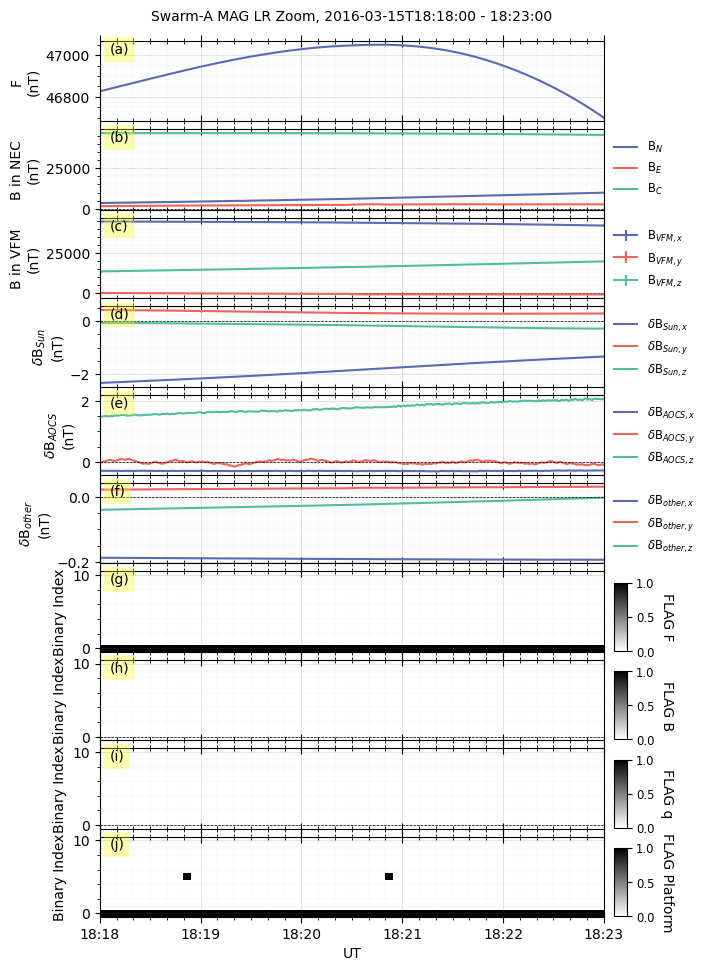
\includegraphics[width=0.7\linewidth]{files/a215a1b350897a52e3808de731f33756.png}

\section{Tutorials}

\subsection{Swarm data access}

This tutorial demonstrates how to access Swarm data using GeospaceLAB. We will use the Swarm MAG LR dataset as an example, but the same process applies to other datasets as well.
A full list of the supported datasets and their name patterns can be found in the \href{/supported-datasets}{Supported datasets} tutorial. Also, the examples for accessing other datasets can be found in the \href{/example-swarm-mag}{Examples} tutorial.

\begin{framed}
\textbf{Tip}\\
In addtion to the examples shown in this documentation, more example scripts can be found in GeospaceLAB \href{https://github.com/JouleCai/geospacelab/tree/master/examples}{examples} and \href{https://github.com/JouleCai/geospacelab/tree/master/test}{test}.
\end{framed}

The Swarm data can be accessed in three ways:

\begin{enumerate}
\item via~Swarm~Dissemination~Server
\item via~Swarm~VirES
\item via~Swarm~VirES~HAPI~Service
\end{enumerate}

\begin{framed}
\textbf{Note}\\
For 2 and 3, GeospaceLAB currently supports only the MAG LR data. Supports for other data products will be implemented next.
\end{framed}

\begin{verbatim}
import datetime
import geospacelab.datahub as datahub
\end{verbatim}

\subsubsection{Access data via Swarm Dissemination Sever}\label{swarm-dissemination-server}

\paragraph{Initial settings}

\begin{verbatim}
dt_fr = datetime.datetime(2016, 3, 15, 18, 18)
dt_to = datetime.datetime(2016, 3, 15, 18, 23)
sat_id = "A"
\end{verbatim}

\paragraph{Create a datahub}

\begin{verbatim}
dh = datahub.DataHub(
    dt_fr=dt_fr,    # Start time for data retrieval
    dt_to=dt_to,    # End time for data retrieval
    visual='on'     # Enable plotting properties for datasets and variables. 
                    # Used for visualizing the data in the dashboard.
    )
\end{verbatim}

\begin{framed}
\textbf{Tip}\\
Above returns a \texttt{DataHub} object, which is used as a data manager in GeospaceLAB. A \texttt{DataHub} object (here is \texttt{dh}) can manage multiple datasets (GeospaceLAB \texttt{Dataset} objects) and a \texttt{Dataset} object manages multiple variables (GeospaceLAB \texttt{Variable} objects).
\end{framed}

\paragraph{Dock a Swarm dataset}

The \texttt{dock} method is called to dock a specific dataset. The \texttt{dock} method responds to a sequence of work flows, including

\begin{itemize}
\item contacting the Swarm Dissemination FTP Sever,
\item checking the data product version and data availability,
\item downloading the data files,
\item loading the data files to the dataset.
\end{itemize}

The method takes the name patterns of the dataset as an argument and returns a dataset object. For example, the following code docks the Swarm MAG LR dataset for the specified time range and satellite ID as shwon above. A full list of the supported datasets and required inputs can be found in the \href{/supported-datasets}{Supported datasets} tutorial.

\begin{verbatim}
ds = dh.dock(
    datasource_contents=['esa_eo', 'swarm', 'l1b', 'mag_lr'],  # The name patterns of the data products to be retrieved.
    sat_id=sat_id,  # The Swarm satellite ID (A, B, or C) for which the data products will be retrieved.
    product_version='latest',  # The version of the data products to be retrieved.
                            # Default is 'latest', which retrieves the most recent version available.
                            # To specify a particular version, use the format 'XXXX' (e.g., '0301').
    add_APEX=True,  # Whether to add APEX coordinates to the dataset.
    )
\end{verbatim}

\begin{verbatim}
Searching the data product "MAG_LR" with the version "latest" on the server...
The file [PosixPath('/data/afys -ionosphere/data/ESA/SWARM/Level1b/MAG_LR/0701/Sat_A/2016/SW_OPER_MAGA_LR_1B_20160315T000000_20160315T235959_0701_MDR_MAG_LR.cdf'), PosixPath('/data/afys -ionosphere/data/ESA/SWARM/Level1b/MAG_LR/0701/Sat_A/2016/SW_OPER_MAGA_LR_1B_20160315T000000_20160315T235959_0701_ASM_VFM_IC.cdf')] already exists: skip downloading.
WARNING: Multiple files found for the pattern *20160315T000000*20160315T235959*0701*.cdf in the directory /data/afys -ionosphere/data/ESA/SWARM/Level1b/MAG_LR/0701/Sat_A/2016!
/opt/anaconda3/envs/Swarm/lib/python3.12/site -packages/numpy/_core/numeric.py:442: RuntimeWarning: invalid value encountered in cast
  multiarray.copyto(res, fill_value, casting='unsafe')
\end{verbatim}

\begin{framed}
\textbf{Note}\\
The data files downloaded from the Swarm Dissemination FTP Sever are stored in the GeospaceLAB data folder (see \href{/configuration}{Configuration}). The data product with different versions are arranged in separate folders.
\end{framed}

\begin{framed}
\textbf{Tip}\\
To access other supported Swarm data products, check \href{/supported-datasets}{Supported datasets in GeospaceLAB} and replace the keyword \texttt{datasource\_contents=['esa\_eo', 'swarm', 'l1b', 'mag\_lr']} with the corresponding name patterns. For example, to dock the Swarm EFI TCT 2Hz data, use the keyword \texttt{datasource\_contents=['esa\_eo', 'swarm', 'advanced', 'efi\_tct02']}. This is also applied for other datasets supported in GeospaceLAB.
\end{framed}

The data files can be listed by calling

\begin{verbatim}
ds.data_file_paths
\end{verbatim}

\begin{verbatim}
[PosixPath('/data/afys -ionosphere/data/ESA/SWARM/Level1b/MAG_LR/0701/Sat_A/2016/SW_OPER_MAGA_LR_1B_20160315T000000_20160315T235959_0701_MDR_MAG_LR.cdf')]
\end{verbatim}

And the data file versions can be listed by calling

\begin{verbatim}
ds.data_file_versions
\end{verbatim}

\begin{verbatim}
['0701']
\end{verbatim}

\subparagraph{List the variables included in the dataset}

To see the variables loaded in the dataset, call

\begin{verbatim}
ds.list_all_variables()
\end{verbatim}

\begin{verbatim}
Dataset: esa/earthonline | swarm | mag | mag_lr
Printing all of the variables ...
|No.                 |Variable name                 |Variable name (Source)        |Description                                                                                         |
| - - - - - - - - - - - - - - - - - - - -| - - - - - - - - - - - - - - - - - - - - - - - - - - - - - -| - - - - - - - - - - - - - - - - - - - - - - - - - - - - - -| - - - - - - - - - - - - - - - - - - - - - - - - - - - - - - - - - - - - - - - - - - - - - - - - - - - - - - - - - - - - - - - - - - - - - - - - - - - - - - - - - - - - - - - - - - - - - - - - - - - -|
|1                   |SC_DATETIME                   |N/A                           |Time of observation                                                                                 |
|2                   |SYNC_STATUS                   |SyncStatus                    |                                                                                                    |
|3                   |SC_GEO_LAT                    |Latitude                      |Geographic Latitude                                                                                 |
|4                   |SC_GEO_LON                    |Longitude                     |Geographic Longitude                                                                                |
|5                   |SC_GEO_r                      |N/A                           |                                                                                                    |
|6                   |B_VFM                         |B_VFM                         |                                                                                                    |
|7                   |B_VFM_x                       |N/A                           |B in x direction of VFM frame                                                                       |
|8                   |B_VFM_y                       |N/A                           |B in y direction of VFM frame                                                                       |
|9                   |B_VFM_z                       |N/A                           |B in z direction of VFM frame                                                                       |
|10                  |B_VFM_x_err                   |N/A                           |                                                                                                    |
|11                  |B_VFM_y_err                   |N/A                           |                                                                                                    |
|12                  |B_VFM_z_err                   |N/A                           |                                                                                                    |
|13                  |B_NEC                         |B_NEC                         |                                                                                                    |
|14                  |B_N                           |N/A                           |B in northward direction of NEC frame                                                               |
|15                  |B_E                           |N/A                           |B in eastward direction of NEC frame                                                                |
|16                  |B_C                           |N/A                           |B in downward direction of NEC frame                                                                |
|17                  |dB_Sun_VFM                    |dB_Sun                        |                                                                                                    |
|18                  |dB_Sun_VFM_x                  |N/A                           |dB due to Sun induced perturbation in x direction of VFM frame                                      |
|19                  |dB_Sun_VFM_y                  |N/A                           |dB due to Sun induced perturbation in y direction of VFM frame                                      |
|20                  |dB_Sun_VFM_z                  |N/A                           |dB due to Sun induced perturbation in z direction of VFM frame                                      |
|21                  |dB_AOCS_VFM                   |dB_AOCS                       |                                                                                                    |
|22                  |dB_AOCS_VFM_x                 |N/A                           |dB due to AOCS induced perturbation in x direction of VFM frame                                     |
|23                  |dB_AOCS_VFM_y                 |N/A                           |dB due to AOCS induced perturbation in y direction of VFM frame                                     |
|24                  |dB_AOCS_VFM_z                 |N/A                           |dB due to AOCS induced perturbation in z direction of VFM frame                                     |
|25                  |dB_other_VFM                  |dB_other                      |                                                                                                    |
|26                  |dB_other_VFM_x                |N/A                           |dB due to all other sources of perturbation in x direction of VFM frame                             |
|27                  |dB_other_VFM_y                |N/A                           |dB due to all other sources of perturbation in y direction of VFM frame                             |
|28                  |dB_other_VFM_z                |N/A                           |dB due to all other sources of perturbation in z direction of VFM frame                             |
|29                  |B_VFM_err                     |B_error                       |                                                                                                    |
|30                  |q_NEC_CRF                     |q_NEC_CRF                     |                                                                                                    |
|31                  |Att_error                     |Att_error                     |                                                                                                    |
|32                  |FLAG_B                        |Flags_B                       |Flag B                                                                                              |
|33                  |FLAG_q                        |Flags_q                       |Flag q                                                                                              |
|34                  |FLAG_Platform                 |Flags_Platform                |Flag Platform                                                                                       |
|35                  |FLAG_B_BIN_AUX                |N/A                           |Binary flag for B                                                                                   |
|36                  |FLAG_B_BIN_IND                |N/A                           |                                                                                                    |
|37                  |FLAG_q_BIN_AUX                |N/A                           |Binary flag for q                                                                                   |
|38                  |FLAG_q_BIN_IND                |N/A                           |                                                                                                    |
|39                  |FLAG_Platform_BIN_AUX         |N/A                           |Binary flag for Platform                                                                            |
|40                  |FLAG_Platform_BIN_IND         |N/A                           |                                                                                                    |
|41                  |FLAG_F                        |Flags_F                       |Flag F                                                                                              |
|42                  |FLAG_F_BIN_AUX                |N/A                           |Binary flag for F                                                                                   |
|43                  |FLAG_F_BIN_IND                |N/A                           |                                                                                                    |
|44                  |ASM_Freq_Dev                  |ASM_Freq_Dev                  |                                                                                                    |
|45                  |F                             |F                             |Magnetic field intensity                                                                            |
|46                  |F_err                         |F_error                       |                                                                                                    |
|47                  |dF_Sun                        |dF_Sun                        |                                                                                                    |
|48                  |dF_AOCS                       |dF_AOCS                       |                                                                                                    |
|49                  |dF_other                      |dF_other                      |                                                                                                    |
|50                  |SC_APEX_LAT                   |N/A                           |APEX Latitude                                                                                       |
|51                  |SC_APEX_LON                   |N/A                           |APEX Longitude                                                                                      |
|52                  |SC_APEX_MLT                   |N/A                           |APEX Magnetic Local Time                                                                            |
|53                  |SC_GEO_LST                    |N/A                           |Local Solar Time                                                                                    |
\end{verbatim}

\subparagraph{Get a variable and data array}

\begin{verbatim}
B_N = ds['B_N']
\end{verbatim}

Above returns a GeospaceLAB Variable object. To get the data array, call

\begin{verbatim}
B_N_arr = B_N.value
\end{verbatim}

Above returns a \texttt{numpy.ndarray} data array.

It is also posible to get the variable using the variable name in the source file/data as shown in the list above:

\begin{verbatim}
ds['SC_GEO_LAT'] == ds['Latitude']
\end{verbatim}

\begin{verbatim}
True
\end{verbatim}

\subsubsection{Access data via Swarm VirES (developing)}\label{swarm-vires}

In a similar way, users can dock the Swarm data product from the Swarm VirES service, by simply adding the keyword \texttt{from\_VirES=True}. It is also possible to access the Swarm FAST data by add the keyword \texttt{from\_FAST=True}.

\begin{framed}
\textbf{Note}\\
Support for the FAST data is only availble when \texttt{from\_VirES=True} or \texttt{from\_HAPI=True} is called.
\end{framed}

\paragraph{Retreive data from VirES}

\begin{verbatim}
ds_VirES = dh.dock(
    datasource_contents=['esa_eo', 'swarm', 'l1b', 'mag_lr'], 
    sat_id=sat_id,
    from_VirES=True,  # Whether to retrieve the data from VirES instead of the local cache. 
    )
ds_VirES.list_all_variables()
\end{verbatim}

\begin{verbatim}
INFO: Loading data from VirES for collection SW_OPER_MAGA_LR_1B with products {'measurements': ['B_VFM', 'B_NEC', 'dB_Sun', 'dB_AOCS', 'dB_other', 'B_error', 'q_NEC_CRF', 'Att_error', 'Flags_B', 'Flags_q', 'Flags_Platform', 'Flags_F', 'ASM_Freq_Dev', 'F', 'F_error', 'dF_Sun', 'dF_AOCS', 'dF_other'], 'models': ['CHAOS -Core'], 'residuals': False}.
Processing:  100%|██████████|  [ Elapsed: 00:00, Remaining: 00:00 ] [1/1] 
Downloading: 100%|██████████|  [ Elapsed: 00:00, Remaining: 00:00 ] (0.219MB)
INFO: Data loaded from VirES.
WARNING: Variable name Spacecraft not found in the variable name dictionary, and no unique match found. Skipping this variable.
WARNING: Variable SC_GEO_R is not in the default variable names and does not match the patterns for automatically assigning configured variable names. It will be added without a configured variable name, and may not be included in the default panels for plotting and analysis. Please check if this variable should be included in the default variable names or if it follows the naming patterns for automatic assignment of configured variable names.
WARNING: Variable B_NEC_CHAOS -Core is not in the default variable names and does not match the patterns for automatically assigning configured variable names. It will be added without a configured variable name, and may not be included in the default panels for plotting and analysis. Please check if this variable should be included in the default variable names or if it follows the naming patterns for automatic assignment of configured variable names.
/opt/anaconda3/envs/Swarm/lib/python3.12/site -packages/numpy/_core/numeric.py:442: RuntimeWarning: invalid value encountered in cast
  multiarray.copyto(res, fill_value, casting='unsafe')
Dataset: esa/earthonline | swarm | mag | mag_lr
Printing all of the variables ...
|No.                 |Variable name                 |Variable name (Source)        |Description                                                                                         |
| - - - - - - - - - - - - - - - - - - - -| - - - - - - - - - - - - - - - - - - - - - - - - - - - - - -| - - - - - - - - - - - - - - - - - - - - - - - - - - - - - -| - - - - - - - - - - - - - - - - - - - - - - - - - - - - - - - - - - - - - - - - - - - - - - - - - - - - - - - - - - - - - - - - - - - - - - - - - - - - - - - - - - - - - - - - - - - - - - - - - - - -|
|1                   |F_err                         |F_error                       |                                                                                                    |
|2                   |dF_Sun                        |dF_Sun                        |                                                                                                    |
|3                   |ASM_Freq_Dev                  |ASM_Freq_Dev                  |                                                                                                    |
|4                   |SC_GEO_R                      |Radius                        |                                                                                                    |
|5                   |FLAG_F                        |Flags_F                       |Flag F                                                                                              |
|6                   |SC_GEO_LON                    |Longitude                     |Geographic Longitude                                                                                |
|7                   |F_CHAOS -Core                  |N/A                           |Magnetic field intensity                                                                            |
|8                   |FLAG_q                        |Flags_q                       |Flag q                                                                                              |
|9                   |FLAG_Platform                 |Flags_Platform                |Flag Platform                                                                                       |
|10                  |dF_AOCS                       |dF_AOCS                       |                                                                                                    |
|11                  |B_NEC_CHAOS -Core              |N/A                           |                                                                                                    |
|12                  |dB_AOCS_VFM                   |dB_AOCS                       |                                                                                                    |
|13                  |dB_other_VFM                  |dB_other                      |                                                                                                    |
|14                  |SC_GEO_LAT                    |Latitude                      |Geographic Latitude                                                                                 |
|15                  |FLAG_B                        |Flags_B                       |Flag B                                                                                              |
|16                  |B_NEC                         |B_NEC                         |                                                                                                    |
|17                  |dB_Sun_VFM                    |dB_Sun                        |                                                                                                    |
|18                  |dF_other                      |dF_other                      |                                                                                                    |
|19                  |q_NEC_CRF                     |q_NEC_CRF                     |                                                                                                    |
|20                  |B_VFM_err                     |B_error                       |                                                                                                    |
|21                  |F                             |F                             |Magnetic field intensity                                                                            |
|22                  |B_VFM                         |B_VFM                         |                                                                                                    |
|23                  |Att_error                     |Att_error                     |                                                                                                    |
|24                  |SC_DATETIME                   |N/A                           |Time of observation                                                                                 |
|25                  |SC_GEO_r                      |N/A                           |                                                                                                    |
|26                  |B_CHAOS -Core_N                |N/A                           |B in northward direction of NEC frame                                                               |
|27                  |B_CHAOS -Core_E                |N/A                           |B in eastward direction of NEC frame                                                                |
|28                  |B_CHAOS -Core_C                |N/A                           |B in downward direction of NEC frame                                                                |
|29                  |dB_AOCS_VFM_x                 |N/A                           |dB due to AOCS induced perturbation in x direction of VFM frame                                     |
|30                  |dB_AOCS_VFM_y                 |N/A                           |dB due to AOCS induced perturbation in y direction of VFM frame                                     |
|31                  |dB_AOCS_VFM_z                 |N/A                           |dB due to AOCS induced perturbation in z direction of VFM frame                                     |
|32                  |dB_other_VFM_x                |N/A                           |dB due to all other sources of perturbation in x direction of VFM frame                             |
|33                  |dB_other_VFM_y                |N/A                           |dB due to all other sources of perturbation in y direction of VFM frame                             |
|34                  |dB_other_VFM_z                |N/A                           |dB due to all other sources of perturbation in z direction of VFM frame                             |
|35                  |B_N                           |N/A                           |B in northward direction of NEC frame                                                               |
|36                  |B_E                           |N/A                           |B in eastward direction of NEC frame                                                                |
|37                  |B_C                           |N/A                           |B in downward direction of NEC frame                                                                |
|38                  |dB_Sun_VFM_x                  |N/A                           |dB due to Sun induced perturbation in x direction of VFM frame                                      |
|39                  |dB_Sun_VFM_y                  |N/A                           |dB due to Sun induced perturbation in y direction of VFM frame                                      |
|40                  |dB_Sun_VFM_z                  |N/A                           |dB due to Sun induced perturbation in z direction of VFM frame                                      |
|41                  |B_VFM_x_err                   |N/A                           |                                                                                                    |
|42                  |B_VFM_y_err                   |N/A                           |                                                                                                    |
|43                  |B_VFM_z_err                   |N/A                           |                                                                                                    |
|44                  |B_VFM_x                       |N/A                           |B in x direction of VFM frame                                                                       |
|45                  |B_VFM_y                       |N/A                           |B in y direction of VFM frame                                                                       |
|46                  |B_VFM_z                       |N/A                           |B in z direction of VFM frame                                                                       |
|47                  |FLAG_B_BIN_AUX                |N/A                           |Binary flag for B                                                                                   |
|48                  |FLAG_B_BIN_IND                |N/A                           |                                                                                                    |
|49                  |FLAG_q_BIN_AUX                |N/A                           |Binary flag for q                                                                                   |
|50                  |FLAG_q_BIN_IND                |N/A                           |                                                                                                    |
|51                  |FLAG_Platform_BIN_AUX         |N/A                           |Binary flag for Platform                                                                            |
|52                  |FLAG_Platform_BIN_IND         |N/A                           |                                                                                                    |
|53                  |FLAG_F_BIN_AUX                |N/A                           |Binary flag for F                                                                                   |
|54                  |FLAG_F_BIN_IND                |N/A                           |                                                                                                    |
|55                  |SC_GEO_LST                    |N/A                           |Local Solar Time                                                                                    |
\end{verbatim}

\paragraph{Retrieve FAST data from VirES}

\begin{verbatim}
dt_now = datetime.datetime.now()
dt_fr_FAST = datetime.datetime(dt_now.year, dt_now.month, dt_now.day) - datetime.timedelta(days=30)
dt_to_FAST = datetime.datetime(dt_now.year, dt_now.month, dt_now.day) - datetime.timedelta(days=30) \
    + datetime.timedelta(hours=0, minutes=2)
ds_VirES_FAST = dh.dock(
    datasource_contents=['esa_eo', 'swarm', 'l1b', 'mag_lr'], 
    dt_fr=dt_fr_FAST,    # Start time for data retrieval
    dt_to=dt_to_FAST,    # End time for data retrieval
    sat_id=sat_id,
    from_VirES=True,  # Whether to retrieve the data from VirES instead of the local cache. 
    from_FAST=True  # Whether to retrieve the data from FAST instead of the local cache.
    )
ds_VirES_FAST.list_all_variables()
\end{verbatim}

\begin{verbatim}
INFO: Loading data from VirES for collection SW_FAST_MAGA_LR_1B with products {'measurements': ['B_VFM', 'B_NEC', 'dB_Sun', 'dB_AOCS', 'dB_other', 'B_error', 'q_NEC_CRF', 'Att_error', 'Flags_B', 'Flags_q', 'Flags_Platform', 'Flags_F', 'ASM_Freq_Dev', 'F', 'F_error', 'dF_Sun', 'dF_AOCS', 'dF_other'], 'models': ['CHAOS -Core'], 'residuals': False}.
Processing:  100%|██████████|  [ Elapsed: 00:00, Remaining: 00:00 ] [1/1] 
Downloading: 100%|██████████|  [ Elapsed: 00:00, Remaining: 00:00 ] (0.217MB)
INFO: Data loaded from VirES.
WARNING: Variable name Spacecraft not found in the variable name dictionary, and no unique match found. Skipping this variable.
WARNING: Variable SC_GEO_R is not in the default variable names and does not match the patterns for automatically assigning configured variable names. It will be added without a configured variable name, and may not be included in the default panels for plotting and analysis. Please check if this variable should be included in the default variable names or if it follows the naming patterns for automatic assignment of configured variable names.
WARNING: Variable B_NEC_CHAOS -Core is not in the default variable names and does not match the patterns for automatically assigning configured variable names. It will be added without a configured variable name, and may not be included in the default panels for plotting and analysis. Please check if this variable should be included in the default variable names or if it follows the naming patterns for automatic assignment of configured variable names.
/opt/anaconda3/envs/Swarm/lib/python3.12/site -packages/numpy/_core/numeric.py:442: RuntimeWarning: invalid value encountered in cast
  multiarray.copyto(res, fill_value, casting='unsafe')
Dataset: esa/earthonline | swarm | mag | mag_lr
Printing all of the variables ...
|No.                 |Variable name                 |Variable name (Source)        |Description                                                                                         |
| - - - - - - - - - - - - - - - - - - - -| - - - - - - - - - - - - - - - - - - - - - - - - - - - - - -| - - - - - - - - - - - - - - - - - - - - - - - - - - - - - -| - - - - - - - - - - - - - - - - - - - - - - - - - - - - - - - - - - - - - - - - - - - - - - - - - - - - - - - - - - - - - - - - - - - - - - - - - - - - - - - - - - - - - - - - - - - - - - - - - - - -|
|1                   |F_err                         |F_error                       |                                                                                                    |
|2                   |dF_Sun                        |dF_Sun                        |                                                                                                    |
|3                   |ASM_Freq_Dev                  |ASM_Freq_Dev                  |                                                                                                    |
|4                   |SC_GEO_R                      |Radius                        |                                                                                                    |
|5                   |FLAG_F                        |Flags_F                       |Flag F                                                                                              |
|6                   |SC_GEO_LON                    |Longitude                     |Geographic Longitude                                                                                |
|7                   |F_CHAOS -Core                  |N/A                           |Magnetic field intensity                                                                            |
|8                   |FLAG_q                        |Flags_q                       |Flag q                                                                                              |
|9                   |FLAG_Platform                 |Flags_Platform                |Flag Platform                                                                                       |
|10                  |dF_AOCS                       |dF_AOCS                       |                                                                                                    |
|11                  |B_NEC_CHAOS -Core              |N/A                           |                                                                                                    |
|12                  |dB_AOCS_VFM                   |dB_AOCS                       |                                                                                                    |
|13                  |dB_other_VFM                  |dB_other                      |                                                                                                    |
|14                  |SC_GEO_LAT                    |Latitude                      |Geographic Latitude                                                                                 |
|15                  |FLAG_B                        |Flags_B                       |Flag B                                                                                              |
|16                  |B_NEC                         |B_NEC                         |                                                                                                    |
|17                  |dB_Sun_VFM                    |dB_Sun                        |                                                                                                    |
|18                  |dF_other                      |dF_other                      |                                                                                                    |
|19                  |q_NEC_CRF                     |q_NEC_CRF                     |                                                                                                    |
|20                  |B_VFM_err                     |B_error                       |                                                                                                    |
|21                  |F                             |F                             |Magnetic field intensity                                                                            |
|22                  |B_VFM                         |B_VFM                         |                                                                                                    |
|23                  |Att_error                     |Att_error                     |                                                                                                    |
|24                  |SC_DATETIME                   |N/A                           |Time of observation                                                                                 |
|25                  |SC_GEO_r                      |N/A                           |                                                                                                    |
|26                  |B_CHAOS -Core_N                |N/A                           |B in northward direction of NEC frame                                                               |
|27                  |B_CHAOS -Core_E                |N/A                           |B in eastward direction of NEC frame                                                                |
|28                  |B_CHAOS -Core_C                |N/A                           |B in downward direction of NEC frame                                                                |
|29                  |dB_AOCS_VFM_x                 |N/A                           |dB due to AOCS induced perturbation in x direction of VFM frame                                     |
|30                  |dB_AOCS_VFM_y                 |N/A                           |dB due to AOCS induced perturbation in y direction of VFM frame                                     |
|31                  |dB_AOCS_VFM_z                 |N/A                           |dB due to AOCS induced perturbation in z direction of VFM frame                                     |
|32                  |dB_other_VFM_x                |N/A                           |dB due to all other sources of perturbation in x direction of VFM frame                             |
|33                  |dB_other_VFM_y                |N/A                           |dB due to all other sources of perturbation in y direction of VFM frame                             |
|34                  |dB_other_VFM_z                |N/A                           |dB due to all other sources of perturbation in z direction of VFM frame                             |
|35                  |B_N                           |N/A                           |B in northward direction of NEC frame                                                               |
|36                  |B_E                           |N/A                           |B in eastward direction of NEC frame                                                                |
|37                  |B_C                           |N/A                           |B in downward direction of NEC frame                                                                |
|38                  |dB_Sun_VFM_x                  |N/A                           |dB due to Sun induced perturbation in x direction of VFM frame                                      |
|39                  |dB_Sun_VFM_y                  |N/A                           |dB due to Sun induced perturbation in y direction of VFM frame                                      |
|40                  |dB_Sun_VFM_z                  |N/A                           |dB due to Sun induced perturbation in z direction of VFM frame                                      |
|41                  |B_VFM_x_err                   |N/A                           |                                                                                                    |
|42                  |B_VFM_y_err                   |N/A                           |                                                                                                    |
|43                  |B_VFM_z_err                   |N/A                           |                                                                                                    |
|44                  |B_VFM_x                       |N/A                           |B in x direction of VFM frame                                                                       |
|45                  |B_VFM_y                       |N/A                           |B in y direction of VFM frame                                                                       |
|46                  |B_VFM_z                       |N/A                           |B in z direction of VFM frame                                                                       |
|47                  |FLAG_B_BIN_AUX                |N/A                           |Binary flag for B                                                                                   |
|48                  |FLAG_B_BIN_IND                |N/A                           |                                                                                                    |
|49                  |FLAG_q_BIN_AUX                |N/A                           |Binary flag for q                                                                                   |
|50                  |FLAG_q_BIN_IND                |N/A                           |                                                                                                    |
|51                  |FLAG_Platform_BIN_AUX         |N/A                           |Binary flag for Platform                                                                            |
|52                  |FLAG_Platform_BIN_IND         |N/A                           |                                                                                                    |
|53                  |FLAG_F_BIN_AUX                |N/A                           |Binary flag for F                                                                                   |
|54                  |FLAG_F_BIN_IND                |N/A                           |                                                                                                    |
|55                  |SC_GEO_LST                    |N/A                           |Local Solar Time                                                                                    |
\end{verbatim}

\subsubsection{Access data via Swarm VirES HAPI Service (developing)}\label{swarm-hapi}

Users can dock the Swarm data product from the VirES HAPI service, by simply adding the keyword \texttt{from\_HAPI=True}.

\paragraph{Retrieve data from HAPI}

\begin{verbatim}
ds_HAPI = dh.dock(
    datasource_contents=['esa_eo', 'swarm', 'l1b', 'mag_lr'], 
    sat_id=sat_id,
    from_HAPI=True,  # Whether to retrieve the data from HAPI instead of the local cache. 
    )
ds_HAPI.list_all_variables()
\end{verbatim}

\begin{verbatim}
INFO: Loading data from HAPI for server https://vires.services/hapi, dataset SW_OPER_MAGA_LR_1B, parameters Timestamp,Latitude,Longitude,Radius.
INFO: Data loaded from HAPI.
INFO: Loading data from HAPI for server https://vires.services/hapi, dataset SW_OPER_MAGA_LR_1B, parameters F,dF_Sun,dF_AOCS,dF_other,F_error,B_VFM,B_NEC,dB_Sun,dB_AOCS,dB_other,B_error.
INFO: Data loaded from HAPI.
INFO: Loading data from HAPI for server https://vires.services/hapi, dataset SW_OPER_MAGA_LR_1B, parameters q_NEC_CRF,Att_error,Flags_F,Flags_B,Flags_q,Flags_Platform,ASM_Freq_Dev.
INFO: Data loaded from HAPI.
INFO: Loading data from HAPI for server https://vires.services/hapi, dataset SW_OPER_MAGA_LR_1B, parameters SyncStatus,B_NEC_Model,F_Model,F_res_Model,B_NEC_res_Model.
INFO: Data loaded from HAPI.
WARNING: Variable CDF_EPOCH is not in the default variable names and does not match the patterns for automatically assigning configured variable names. It will be added without a configured variable name, and may not be included in the default panels for plotting and analysis. Please check if this variable should be included in the default variable names or if it follows the naming patterns for automatic assignment of configured variable names.
WARNING: Variable SC_GEO_R is not in the default variable names and does not match the patterns for automatically assigning configured variable names. It will be added without a configured variable name, and may not be included in the default panels for plotting and analysis. Please check if this variable should be included in the default variable names or if it follows the naming patterns for automatic assignment of configured variable names.
WARNING: Variable B_NEC_Model is not in the default variable names and does not match the patterns for automatically assigning configured variable names. It will be added without a configured variable name, and may not be included in the default panels for plotting and analysis. Please check if this variable should be included in the default variable names or if it follows the naming patterns for automatic assignment of configured variable names.
WARNING: Variable B_NEC_res_Model is not in the default variable names and does not match the patterns for automatically assigning configured variable names. It will be added without a configured variable name, and may not be included in the default panels for plotting and analysis. Please check if this variable should be included in the default variable names or if it follows the naming patterns for automatic assignment of configured variable names.
/opt/anaconda3/envs/Swarm/lib/python3.12/site -packages/numpy/_core/numeric.py:476: RuntimeWarning: invalid value encountered in cast
  multiarray.copyto(res, fill_value, casting='unsafe')
Dataset: esa/earthonline | swarm | mag | mag_lr
Printing all of the variables ...
|No.                 |Variable name                 |Variable name (Source)        |Description                                                                                         |
| - - - - - - - - - - - - - - - - - - - -| - - - - - - - - - - - - - - - - - - - - - - - - - - - - - -| - - - - - - - - - - - - - - - - - - - - - - - - - - - - - -| - - - - - - - - - - - - - - - - - - - - - - - - - - - - - - - - - - - - - - - - - - - - - - - - - - - - - - - - - - - - - - - - - - - - - - - - - - - - - - - - - - - - - - - - - - - - - - - - - - - -|
|1                   |CDF_EPOCH                     |Timestamp                     |                                                                                                    |
|2                   |SC_GEO_LAT                    |Latitude                      |Geographic Latitude                                                                                 |
|3                   |SC_GEO_LON                    |Longitude                     |Geographic Longitude                                                                                |
|4                   |SC_GEO_R                      |Radius                        |                                                                                                    |
|5                   |SC_DATETIME                   |N/A                           |Time of observation                                                                                 |
|6                   |F                             |F                             |Magnetic field intensity                                                                            |
|7                   |dF_Sun                        |dF_Sun                        |                                                                                                    |
|8                   |dF_AOCS                       |dF_AOCS                       |                                                                                                    |
|9                   |dF_other                      |dF_other                      |                                                                                                    |
|10                  |F_err                         |F_error                       |                                                                                                    |
|11                  |B_VFM                         |B_VFM                         |                                                                                                    |
|12                  |B_NEC                         |B_NEC                         |                                                                                                    |
|13                  |dB_Sun_VFM                    |dB_Sun                        |                                                                                                    |
|14                  |dB_AOCS_VFM                   |dB_AOCS                       |                                                                                                    |
|15                  |dB_other_VFM                  |dB_other                      |                                                                                                    |
|16                  |B_VFM_err                     |B_error                       |                                                                                                    |
|17                  |q_NEC_CRF                     |q_NEC_CRF                     |                                                                                                    |
|18                  |Att_error                     |Att_error                     |                                                                                                    |
|19                  |FLAG_F                        |Flags_F                       |Flag F                                                                                              |
|20                  |FLAG_B                        |Flags_B                       |Flag B                                                                                              |
|21                  |FLAG_q                        |Flags_q                       |Flag q                                                                                              |
|22                  |FLAG_Platform                 |Flags_Platform                |Flag Platform                                                                                       |
|23                  |ASM_Freq_Dev                  |ASM_Freq_Dev                  |                                                                                                    |
|24                  |SYNC_STATUS                   |SyncStatus                    |                                                                                                    |
|25                  |B_NEC_Model                   |N/A                           |                                                                                                    |
|26                  |F_Model                       |N/A                           |Magnetic field intensity                                                                            |
|27                  |F_res_Model                   |N/A                           |Magnetic field intensity                                                                            |
|28                  |B_NEC_res_Model               |N/A                           |                                                                                                    |
|29                  |SC_GEO_r                      |N/A                           |                                                                                                    |
|30                  |B_VFM_x                       |N/A                           |B in x direction of VFM frame                                                                       |
|31                  |B_VFM_y                       |N/A                           |B in y direction of VFM frame                                                                       |
|32                  |B_VFM_z                       |N/A                           |B in z direction of VFM frame                                                                       |
|33                  |B_N                           |N/A                           |B in northward direction of NEC frame                                                               |
|34                  |B_E                           |N/A                           |B in eastward direction of NEC frame                                                                |
|35                  |B_C                           |N/A                           |B in downward direction of NEC frame                                                                |
|36                  |dB_Sun_VFM_x                  |N/A                           |dB due to Sun induced perturbation in x direction of VFM frame                                      |
|37                  |dB_Sun_VFM_y                  |N/A                           |dB due to Sun induced perturbation in y direction of VFM frame                                      |
|38                  |dB_Sun_VFM_z                  |N/A                           |dB due to Sun induced perturbation in z direction of VFM frame                                      |
|39                  |dB_AOCS_VFM_x                 |N/A                           |dB due to AOCS induced perturbation in x direction of VFM frame                                     |
|40                  |dB_AOCS_VFM_y                 |N/A                           |dB due to AOCS induced perturbation in y direction of VFM frame                                     |
|41                  |dB_AOCS_VFM_z                 |N/A                           |dB due to AOCS induced perturbation in z direction of VFM frame                                     |
|42                  |dB_other_VFM_x                |N/A                           |dB due to all other sources of perturbation in x direction of VFM frame                             |
|43                  |dB_other_VFM_y                |N/A                           |dB due to all other sources of perturbation in y direction of VFM frame                             |
|44                  |dB_other_VFM_z                |N/A                           |dB due to all other sources of perturbation in z direction of VFM frame                             |
|45                  |B_VFM_x_err                   |N/A                           |                                                                                                    |
|46                  |B_VFM_y_err                   |N/A                           |                                                                                                    |
|47                  |B_VFM_z_err                   |N/A                           |                                                                                                    |
|48                  |B_Model_N                     |N/A                           |B in northward direction of NEC frame                                                               |
|49                  |B_Model_E                     |N/A                           |B in eastward direction of NEC frame                                                                |
|50                  |B_Model_C                     |N/A                           |B in downward direction of NEC frame                                                                |
|51                  |B_res_Model_N                 |N/A                           |B in northward direction of NEC frame                                                               |
|52                  |B_res_Model_E                 |N/A                           |B in eastward direction of NEC frame                                                                |
|53                  |B_res_Model_C                 |N/A                           |B in downward direction of NEC frame                                                                |
|54                  |FLAG_B_BIN_AUX                |N/A                           |Binary flag for B                                                                                   |
|55                  |FLAG_B_BIN_IND                |N/A                           |                                                                                                    |
|56                  |FLAG_q_BIN_AUX                |N/A                           |Binary flag for q                                                                                   |
|57                  |FLAG_q_BIN_IND                |N/A                           |                                                                                                    |
|58                  |FLAG_Platform_BIN_AUX         |N/A                           |Binary flag for Platform                                                                            |
|59                  |FLAG_Platform_BIN_IND         |N/A                           |                                                                                                    |
|60                  |FLAG_F_BIN_AUX                |N/A                           |Binary flag for F                                                                                   |
|61                  |FLAG_F_BIN_IND                |N/A                           |                                                                                                    |
|62                  |SC_GEO_LST                    |N/A                           |Local Solar Time                                                                                    |
\end{verbatim}

\paragraph{Retrieve FAST data from HAPI}

\begin{verbatim}
dt_now = datetime.datetime.now()
dt_fr_FAST = datetime.datetime(dt_now.year, dt_now.month, dt_now.day) - datetime.timedelta(days=30)
dt_to_FAST = datetime.datetime(dt_now.year, dt_now.month, dt_now.day) - datetime.timedelta(days=30) \
    + datetime.timedelta(hours=0, minutes=2)
ds_HAPI_FAST = dh.dock(
    datasource_contents=['esa_eo', 'swarm', 'l1b', 'mag_lr'], 
    dt_fr=dt_fr_FAST,    # Start time for data retrieval
    dt_to=dt_to_FAST,    # End time for data retrieval
    sat_id=sat_id,
    from_HAPI=True,  # Whether to retrieve the data from HAPI instead of the local cache. 
    from_FAST=True  # Whether to retrieve the data from FAST instead of the local cache.
    )
ds_HAPI_FAST.list_all_variables()
\end{verbatim}

\begin{verbatim}
INFO: Loading data from HAPI for server https://vires.services/hapi, dataset SW_FAST_MAGA_LR_1B, parameters Timestamp,Latitude,Longitude,Radius.
INFO: Data loaded from HAPI.
INFO: Loading data from HAPI for server https://vires.services/hapi, dataset SW_FAST_MAGA_LR_1B, parameters F,dF_Sun,dF_AOCS,dF_other,F_error,B_VFM,B_NEC,dB_Sun,dB_AOCS,dB_other,B_error.
INFO: Data loaded from HAPI.
INFO: Loading data from HAPI for server https://vires.services/hapi, dataset SW_FAST_MAGA_LR_1B, parameters q_NEC_CRF,Att_error,Flags_F,Flags_B,Flags_q,Flags_Platform,ASM_Freq_Dev.
INFO: Data loaded from HAPI.
INFO: Loading data from HAPI for server https://vires.services/hapi, dataset SW_FAST_MAGA_LR_1B, parameters SyncStatus,B_NEC_Model,F_Model,F_res_Model,B_NEC_res_Model.
INFO: Data loaded from HAPI.
WARNING: Variable CDF_EPOCH is not in the default variable names and does not match the patterns for automatically assigning configured variable names. It will be added without a configured variable name, and may not be included in the default panels for plotting and analysis. Please check if this variable should be included in the default variable names or if it follows the naming patterns for automatic assignment of configured variable names.
WARNING: Variable SC_GEO_R is not in the default variable names and does not match the patterns for automatically assigning configured variable names. It will be added without a configured variable name, and may not be included in the default panels for plotting and analysis. Please check if this variable should be included in the default variable names or if it follows the naming patterns for automatic assignment of configured variable names.
WARNING: Variable B_NEC_Model is not in the default variable names and does not match the patterns for automatically assigning configured variable names. It will be added without a configured variable name, and may not be included in the default panels for plotting and analysis. Please check if this variable should be included in the default variable names or if it follows the naming patterns for automatic assignment of configured variable names.
WARNING: Variable B_NEC_res_Model is not in the default variable names and does not match the patterns for automatically assigning configured variable names. It will be added without a configured variable name, and may not be included in the default panels for plotting and analysis. Please check if this variable should be included in the default variable names or if it follows the naming patterns for automatic assignment of configured variable names.
/opt/anaconda3/envs/Swarm/lib/python3.12/site -packages/numpy/_core/numeric.py:442: RuntimeWarning: invalid value encountered in cast
  multiarray.copyto(res, fill_value, casting='unsafe')
Dataset: esa/earthonline | swarm | mag | mag_lr
Printing all of the variables ...
|No.                 |Variable name                 |Variable name (Source)        |Description                                                                                         |
| - - - - - - - - - - - - - - - - - - - -| - - - - - - - - - - - - - - - - - - - - - - - - - - - - - -| - - - - - - - - - - - - - - - - - - - - - - - - - - - - - -| - - - - - - - - - - - - - - - - - - - - - - - - - - - - - - - - - - - - - - - - - - - - - - - - - - - - - - - - - - - - - - - - - - - - - - - - - - - - - - - - - - - - - - - - - - - - - - - - - - - -|
|1                   |CDF_EPOCH                     |Timestamp                     |                                                                                                    |
|2                   |SC_GEO_LAT                    |Latitude                      |Geographic Latitude                                                                                 |
|3                   |SC_GEO_LON                    |Longitude                     |Geographic Longitude                                                                                |
|4                   |SC_GEO_R                      |Radius                        |                                                                                                    |
|5                   |SC_DATETIME                   |N/A                           |Time of observation                                                                                 |
|6                   |F                             |F                             |Magnetic field intensity                                                                            |
|7                   |dF_Sun                        |dF_Sun                        |                                                                                                    |
|8                   |dF_AOCS                       |dF_AOCS                       |                                                                                                    |
|9                   |dF_other                      |dF_other                      |                                                                                                    |
|10                  |F_err                         |F_error                       |                                                                                                    |
|11                  |B_VFM                         |B_VFM                         |                                                                                                    |
|12                  |B_NEC                         |B_NEC                         |                                                                                                    |
|13                  |dB_Sun_VFM                    |dB_Sun                        |                                                                                                    |
|14                  |dB_AOCS_VFM                   |dB_AOCS                       |                                                                                                    |
|15                  |dB_other_VFM                  |dB_other                      |                                                                                                    |
|16                  |B_VFM_err                     |B_error                       |                                                                                                    |
|17                  |q_NEC_CRF                     |q_NEC_CRF                     |                                                                                                    |
|18                  |Att_error                     |Att_error                     |                                                                                                    |
|19                  |FLAG_F                        |Flags_F                       |Flag F                                                                                              |
|20                  |FLAG_B                        |Flags_B                       |Flag B                                                                                              |
|21                  |FLAG_q                        |Flags_q                       |Flag q                                                                                              |
|22                  |FLAG_Platform                 |Flags_Platform                |Flag Platform                                                                                       |
|23                  |ASM_Freq_Dev                  |ASM_Freq_Dev                  |                                                                                                    |
|24                  |SYNC_STATUS                   |SyncStatus                    |                                                                                                    |
|25                  |B_NEC_Model                   |N/A                           |                                                                                                    |
|26                  |F_Model                       |N/A                           |Magnetic field intensity                                                                            |
|27                  |F_res_Model                   |N/A                           |Magnetic field intensity                                                                            |
|28                  |B_NEC_res_Model               |N/A                           |                                                                                                    |
|29                  |SC_GEO_r                      |N/A                           |                                                                                                    |
|30                  |B_VFM_x                       |N/A                           |B in x direction of VFM frame                                                                       |
|31                  |B_VFM_y                       |N/A                           |B in y direction of VFM frame                                                                       |
|32                  |B_VFM_z                       |N/A                           |B in z direction of VFM frame                                                                       |
|33                  |B_N                           |N/A                           |B in northward direction of NEC frame                                                               |
|34                  |B_E                           |N/A                           |B in eastward direction of NEC frame                                                                |
|35                  |B_C                           |N/A                           |B in downward direction of NEC frame                                                                |
|36                  |dB_Sun_VFM_x                  |N/A                           |dB due to Sun induced perturbation in x direction of VFM frame                                      |
|37                  |dB_Sun_VFM_y                  |N/A                           |dB due to Sun induced perturbation in y direction of VFM frame                                      |
|38                  |dB_Sun_VFM_z                  |N/A                           |dB due to Sun induced perturbation in z direction of VFM frame                                      |
|39                  |dB_AOCS_VFM_x                 |N/A                           |dB due to AOCS induced perturbation in x direction of VFM frame                                     |
|40                  |dB_AOCS_VFM_y                 |N/A                           |dB due to AOCS induced perturbation in y direction of VFM frame                                     |
|41                  |dB_AOCS_VFM_z                 |N/A                           |dB due to AOCS induced perturbation in z direction of VFM frame                                     |
|42                  |dB_other_VFM_x                |N/A                           |dB due to all other sources of perturbation in x direction of VFM frame                             |
|43                  |dB_other_VFM_y                |N/A                           |dB due to all other sources of perturbation in y direction of VFM frame                             |
|44                  |dB_other_VFM_z                |N/A                           |dB due to all other sources of perturbation in z direction of VFM frame                             |
|45                  |B_VFM_x_err                   |N/A                           |                                                                                                    |
|46                  |B_VFM_y_err                   |N/A                           |                                                                                                    |
|47                  |B_VFM_z_err                   |N/A                           |                                                                                                    |
|48                  |B_Model_N                     |N/A                           |B in northward direction of NEC frame                                                               |
|49                  |B_Model_E                     |N/A                           |B in eastward direction of NEC frame                                                                |
|50                  |B_Model_C                     |N/A                           |B in downward direction of NEC frame                                                                |
|51                  |B_res_Model_N                 |N/A                           |B in northward direction of NEC frame                                                               |
|52                  |B_res_Model_E                 |N/A                           |B in eastward direction of NEC frame                                                                |
|53                  |B_res_Model_C                 |N/A                           |B in downward direction of NEC frame                                                                |
|54                  |FLAG_B_BIN_AUX                |N/A                           |Binary flag for B                                                                                   |
|55                  |FLAG_B_BIN_IND                |N/A                           |                                                                                                    |
|56                  |FLAG_q_BIN_AUX                |N/A                           |Binary flag for q                                                                                   |
|57                  |FLAG_q_BIN_IND                |N/A                           |                                                                                                    |
|58                  |FLAG_Platform_BIN_AUX         |N/A                           |Binary flag for Platform                                                                            |
|59                  |FLAG_Platform_BIN_IND         |N/A                           |                                                                                                    |
|60                  |FLAG_F_BIN_AUX                |N/A                           |Binary flag for F                                                                                   |
|61                  |FLAG_F_BIN_IND                |N/A                           |                                                                                                    |
|62                  |SC_GEO_LST                    |N/A                           |Local Solar Time                                                                                    |
\end{verbatim}

\subsubsection{Supported datasets in GeospaceLAB}

\begin{verbatim}
import geospacelab.datahub as datahub
dh = datahub.DataHub()
dh.list_sourced_datasets()
\end{verbatim}

\begin{verbatim}
Load IGRF coefficients ...
data_sources
| - - -CDAWEB
| - - -| - - -DMSP
| - - -| - - -| - - -SSUSI
| - - -| - - -| - - -| - - -EDR_AUR
| - - -| - - -| - - -| - - -| - - -Required inputs when load_mode="AUTO": ['datasource_contents']
| - - -| - - -| - - -| - - -| - - -datasource_contents: ['cdaweb', 'dmsp', 'ssusi', 'edr_aur']
| - - -| - - -| - - -| - - -SDR_DISK
| - - -| - - -| - - -| - - -| - - -Required inputs when load_mode="AUTO": ['datasource_contents', 'sat_id', 'orbit_id', 'pp_type', 'pole']
| - - -| - - -| - - -| - - -| - - -datasource_contents: ['cdaweb', 'dmsp', 'ssusi', 'sdr_disk']
| - - -| - - -OMNI
| - - -| - - -| - - -Required inputs when load_mode="AUTO": ['datasource_contents', 'omni_type', 'omni_res']
| - - -| - - -| - - -datasource_contents: ['cdaweb', 'omni']
| - - -ESA_EO
| - - -| - - -SWARM
| - - -| - - -| - - -ADVANCED
| - - -| - - -| - - -| - - -EFI_IDM
| - - -| - - -| - - -| - - -| - - -Required inputs when load_mode="AUTO": ['datasource_contents', 'sat_id']
| - - -| - - -| - - -| - - -| - - -datasource_contents: ['esa_eo', 'swarm', 'advanced', 'efi_idm']
| - - -| - - -| - - -| - - -EFI_LP_FP
| - - -| - - -| - - -| - - -| - - -Required inputs when load_mode="AUTO": ['datasource_contents', 'sat_id']
| - - -| - - -| - - -| - - -| - - -datasource_contents: ['esa_eo', 'swarm', 'advanced', 'efi_lp_fp']
| - - -| - - -| - - -| - - -EFI_LP_HM
| - - -| - - -| - - -| - - -| - - -Required inputs when load_mode="AUTO": ['datasource_contents', 'sat_id']
| - - -| - - -| - - -| - - -| - - -datasource_contents: ['esa_eo', 'swarm', 'advanced', 'efi_lp_hm']
| - - -| - - -| - - -| - - -EFI_TCT02
| - - -| - - -| - - -| - - -| - - -Required inputs when load_mode="AUTO": ['datasource_contents', 'sat_id']
| - - -| - - -| - - -| - - -| - - -datasource_contents: ['esa_eo', 'swarm', 'advanced', 'efi_tct02']
| - - -| - - -| - - -| - - -EFI_TCT16
| - - -| - - -| - - -| - - -| - - -Required inputs when load_mode="AUTO": ['datasource_contents', 'sat_id']
| - - -| - - -| - - -| - - -| - - -datasource_contents: ['esa_eo', 'swarm', 'advanced', 'efi_tct16']
| - - -| - - -| - - -L1B
| - - -| - - -| - - -| - - -EFI_LP
| - - -| - - -| - - -| - - -| - - -Required inputs when load_mode="AUTO": ['datasource_contents', 'sat_id']
| - - -| - - -| - - -| - - -| - - -datasource_contents: ['esa_eo', 'swarm', 'l1b', 'efi_lp']
| - - -| - - -| - - -| - - -EFI_LPI
| - - -| - - -| - - -| - - -| - - -Required inputs when load_mode="AUTO": ['datasource_contents', 'sat_id']
| - - -| - - -| - - -| - - -| - - -datasource_contents: ['esa_eo', 'swarm', 'l1b', 'efi_lpi']
| - - -| - - -| - - -| - - -MAG_HR
| - - -| - - -| - - -| - - -| - - -Required inputs when load_mode="AUTO": ['datasource_contents', 'sat_id']
| - - -| - - -| - - -| - - -| - - -datasource_contents: ['esa_eo', 'swarm', 'l1b', 'mag_hr']
| - - -| - - -| - - -| - - -MAG_LR
| - - -| - - -| - - -| - - -| - - -Required inputs when load_mode="AUTO": ['datasource_contents', 'sat_id']
| - - -| - - -| - - -| - - -| - - -datasource_contents: ['esa_eo', 'swarm', 'l1b', 'mag_lr']
| - - -| - - -| - - -L2DAILY
| - - -| - - -| - - -| - - -AEJ_LPL
| - - -| - - -| - - -| - - -| - - -Required inputs when load_mode="AUTO": ['datasource_contents', 'sat_id']
| - - -| - - -| - - -| - - -| - - -datasource_contents: ['esa_eo', 'swarm', 'l2daily', 'aej_lpl']
| - - -| - - -| - - -| - - -AEJ_PBL
| - - -| - - -| - - -| - - -| - - -Required inputs when load_mode="AUTO": ['datasource_contents', 'sat_id']
| - - -| - - -| - - -| - - -| - - -datasource_contents: ['esa_eo', 'swarm', 'l2daily', 'aej_pbl']
| - - -| - - -| - - -| - - -AEJ_PBS
| - - -| - - -| - - -| - - -| - - -Required inputs when load_mode="AUTO": ['datasource_contents', 'sat_id']
| - - -| - - -| - - -| - - -| - - -datasource_contents: ['esa_eo', 'swarm', 'l2daily', 'aej_pbs']
| - - -| - - -| - - -| - - -AOB_FAC
| - - -| - - -| - - -| - - -| - - -Required inputs when load_mode="AUTO": ['datasource_contents', 'sat_id']
| - - -| - - -| - - -| - - -| - - -datasource_contents: ['esa_eo', 'swarm', 'l2daily', 'aob_fac']
| - - -| - - -| - - -| - - -DNS_ACC
| - - -| - - -| - - -| - - -| - - -Required inputs when load_mode="AUTO": ['datasource_contents', 'sat_id']
| - - -| - - -| - - -| - - -| - - -datasource_contents: ['esa_eo', 'swarm', 'l2daily', 'dns_acc']
| - - -| - - -| - - -| - - -DNS_POD
| - - -| - - -| - - -| - - -| - - -Required inputs when load_mode="AUTO": ['datasource_contents', 'sat_id']
| - - -| - - -| - - -| - - -| - - -datasource_contents: ['esa_eo', 'swarm', 'l2daily', 'dns_pod']
| - - -| - - -| - - -| - - -EEF_TMS
| - - -| - - -| - - -| - - -| - - -Required inputs when load_mode="AUTO": ['datasource_contents', 'sat_id']
| - - -| - - -| - - -| - - -| - - -datasource_contents: ['esa_eo', 'swarm', 'l2daily', 'eef_tms']
| - - -| - - -| - - -| - - -EFI_TIE
| - - -| - - -| - - -| - - -| - - -Required inputs when load_mode="AUTO": ['datasource_contents', 'sat_id']
| - - -| - - -| - - -| - - -| - - -datasource_contents: ['esa_eo', 'swarm', 'l2daily', 'efi_tie']
| - - -| - - -| - - -| - - -FAC_LLS_DUAL
| - - -| - - -| - - -| - - -| - - -Required inputs when load_mode="AUTO": ['datasource_contents']
| - - -| - - -| - - -| - - -| - - -datasource_contents: ['esa_eo', 'swarm', 'l2daily', 'fac_lls_dual']
| - - -| - - -| - - -| - - -FAC_TMS
| - - -| - - -| - - -| - - -| - - -Required inputs when load_mode="AUTO": ['datasource_contents', 'sat_id']
| - - -| - - -| - - -| - - -| - - -datasource_contents: ['esa_eo', 'swarm', 'l2daily', 'fac_tms']
| - - -| - - -| - - -| - - -FAC_TMS_DUAL
| - - -| - - -| - - -| - - -| - - -Required inputs when load_mode="AUTO": ['datasource_contents']
| - - -| - - -| - - -| - - -| - - -datasource_contents: ['esa_eo', 'swarm', 'l2daily', 'fac_tms_dual']
| - - -| - - -| - - -| - - -IBI_TMS
| - - -| - - -| - - -| - - -| - - -Required inputs when load_mode="AUTO": ['datasource_contents', 'sat_id']
| - - -| - - -| - - -| - - -| - - -datasource_contents: ['esa_eo', 'swarm', 'l2daily', 'ibi_tms']
| - - -| - - -| - - -| - - -IPD_IRR
| - - -| - - -| - - -| - - -| - - -Required inputs when load_mode="AUTO": ['datasource_contents', 'sat_id']
| - - -| - - -| - - -| - - -| - - -datasource_contents: ['esa_eo', 'swarm', 'l2daily', 'ipd_irr']
| - - -| - - -| - - -| - - -MIT_LP
| - - -| - - -| - - -| - - -| - - -Required inputs when load_mode="AUTO": ['datasource_contents', 'sat_id']
| - - -| - - -| - - -| - - -| - - -datasource_contents: ['esa_eo', 'swarm', 'l2daily', 'mit_lp']
| - - -| - - -| - - -| - - -MIT_TEC
| - - -| - - -| - - -| - - -| - - -Required inputs when load_mode="AUTO": ['datasource_contents', 'sat_id']
| - - -| - - -| - - -| - - -| - - -datasource_contents: ['esa_eo', 'swarm', 'l2daily', 'mit_tec']
| - - -| - - -| - - -| - - -NIX_TMS
| - - -| - - -| - - -| - - -| - - -Required inputs when load_mode="AUTO": ['datasource_contents', 'sat_id']
| - - -| - - -| - - -| - - -| - - -datasource_contents: ['esa_eo', 'swarm', 'l2daily', 'nix_tms']
| - - -| - - -| - - -| - - -PPI_FAC
| - - -| - - -| - - -| - - -| - - -Required inputs when load_mode="AUTO": ['datasource_contents', 'sat_id']
| - - -| - - -| - - -| - - -| - - -datasource_contents: ['esa_eo', 'swarm', 'l2daily', 'ppi_fac']
| - - -| - - -| - - -| - - -TEC_TMS
| - - -| - - -| - - -| - - -| - - -Required inputs when load_mode="AUTO": ['datasource_contents', 'sat_id']
| - - -| - - -| - - -| - - -| - - -datasource_contents: ['esa_eo', 'swarm', 'l2daily', 'tec_tms']
| - - -| - - -| - - -| - - -TIX_TMS
| - - -| - - -| - - -| - - -| - - -Required inputs when load_mode="AUTO": ['datasource_contents', 'sat_id']
| - - -| - - -| - - -| - - -| - - -datasource_contents: ['esa_eo', 'swarm', 'l2daily', 'tix_tms']
| - - -| - - -| - - -| - - -WHI_EVT
| - - -| - - -| - - -| - - -| - - -Required inputs when load_mode="AUTO": ['datasource_contents', 'sat_id']
| - - -| - - -| - - -| - - -| - - -datasource_contents: ['esa_eo', 'swarm', 'l2daily', 'whi_evt']
| - - -FMI
| - - -| - - -IMAGE
| - - -| - - -| - - -IE
| - - -| - - -| - - -| - - -Required inputs when load_mode="AUTO": ['datasource_contents']
| - - -| - - -| - - -| - - -datasource_contents: ['fmi', 'image', 'ie']
| - - -GFZ
| - - -| - - -HPO
| - - -| - - -| - - -Required inputs when load_mode="AUTO": ['datasource_contents']
| - - -| - - -| - - -datasource_contents: ['gfz', 'hpo']
| - - -| - - -| - - -NOWCAST
| - - -| - - -| - - -| - - -Required inputs when load_mode="AUTO": ['datasource_contents']
| - - -| - - -| - - -| - - -datasource_contents: ['gfz', 'hpo', 'nowcast']
| - - -| - - -KPAP
| - - -| - - -| - - -Required inputs when load_mode="AUTO": ['datasource_contents']
| - - -| - - -| - - -datasource_contents: ['gfz', 'kpap']
| - - -| - - -| - - -NOWCAST
| - - -| - - -| - - -| - - -Required inputs when load_mode="AUTO": ['datasource_contents']
| - - -| - - -| - - -| - - -datasource_contents: ['gfz', 'kpap', 'nowcast']
| - - -| - - -SNF107
| - - -| - - -| - - -Required inputs when load_mode="AUTO": ['datasource_contents']
| - - -| - - -| - - -datasource_contents: ['gfz', 'snf107']
| - - -ISEE
| - - -| - - -GNSS
| - - -| - - -| - - -TECMAP
| - - -| - - -| - - -| - - -Required inputs when load_mode="AUTO": ['datasource_contents']
| - - -| - - -| - - -| - - -datasource_contents: ['isee', 'gnss', 'tecmap']
| - - -JHUAPL
| - - -| - - -AMPERE
| - - -| - - -| - - -FITTED
| - - -| - - -| - - -| - - -Required inputs when load_mode="AUTO": ['datasource_contents']
| - - -| - - -| - - -| - - -datasource_contents: ['jhuapl', 'ampere', 'fitted']
| - - -| - - -| - - -GRD
| - - -| - - -| - - -| - - -Required inputs when load_mode="AUTO": ['datasource_contents']
| - - -| - - -| - - -| - - -datasource_contents: ['jhuapl', 'ampere', 'grd']
| - - -| - - -DMSP
| - - -| - - -| - - -SSUSI
| - - -| - - -| - - -| - - -EDRAUR
| - - -| - - -| - - -| - - -| - - -Required inputs when load_mode="AUTO": ['datasource_contents']
| - - -| - - -| - - -| - - -| - - -datasource_contents: ['jhuapl', 'dmsp', 'ssusi', 'edraur']
| - - -| - - -| - - -| - - -SDRDISK
| - - -| - - -| - - -| - - -| - - -Required inputs when load_mode="AUTO": ['datasource_contents', 'sat_id', 'orbit_id', 'pp_type', 'pole']
| - - -| - - -| - - -| - - -| - - -datasource_contents: ['jhuapl', 'dmsp', 'ssusi', 'sdrdisk']
| - - -MADRIGAL
| - - -| - - -GNSS
| - - -| - - -| - - -TECMAP
| - - -| - - -| - - -| - - -Required inputs when load_mode="AUTO": ['datasource_contents']
| - - -| - - -| - - -| - - -datasource_contents: ['madrigal', 'gnss', 'tecmap']
| - - -| - - -ISR
| - - -| - - -| - - -EISCAT
| - - -| - - -| - - -| - - -Required inputs when load_mode="AUTO": ['datasource_contents', 'site', 'antenna']
| - - -| - - -| - - -| - - -datasource_contents: ['madrigal', 'isr', 'eiscat']
| - - -| - - -| - - -MILLSTONEHILL
| - - -| - - -| - - -| - - -BASIC
| - - -| - - -| - - -| - - -| - - -Required inputs when load_mode="AUTO": ['datasource_contents', 'antenna', 'pulse_code', 'pulse_length']
| - - -| - - -| - - -| - - -| - - -datasource_contents: ['madrigal', 'isr', 'millstonehill', 'basic']
| - - -| - - -| - - -| - - -GRIDDED
| - - -| - - -| - - -| - - -| - - -Required inputs when load_mode="AUTO": ['datasource_contents']
| - - -| - - -| - - -| - - -| - - -datasource_contents: ['madrigal', 'isr', 'millstonehill', 'gridded']
| - - -| - - -| - - -| - - -VI
| - - -| - - -| - - -| - - -| - - -Required inputs when load_mode="AUTO": ['datasource_contents']
| - - -| - - -| - - -| - - -| - - -datasource_contents: ['madrigal', 'isr', 'millstonehill', 'vi']
| - - -| - - -| - - -PFISR
| - - -| - - -| - - -| - - -FITTED
| - - -| - - -| - - -| - - -| - - -Required inputs when load_mode="AUTO": ['datasource_contents']
| - - -| - - -| - - -| - - -| - - -datasource_contents: ['madrigal', 'isr', 'pfisr', 'fitted']
| - - -| - - -| - - -| - - -VI
| - - -| - - -| - - -| - - -| - - -Required inputs when load_mode="AUTO": ['datasource_contents']
| - - -| - - -| - - -| - - -| - - -datasource_contents: ['madrigal', 'isr', 'pfisr', 'vi']
| - - -| - - -| - - -RISR_N
| - - -| - - -| - - -| - - -FITTED
| - - -| - - -| - - -| - - -| - - -Required inputs when load_mode="AUTO": ['datasource_contents']
| - - -| - - -| - - -| - - -| - - -datasource_contents: ['madrigal', 'isr', 'risr_n', 'fitted']
| - - -| - - -| - - -| - - -VI
| - - -| - - -| - - -| - - -| - - -Required inputs when load_mode="AUTO": ['datasource_contents']
| - - -| - - -| - - -| - - -| - - -datasource_contents: ['madrigal', 'isr', 'risr_n', 'vi']
| - - -| - - -SATELLITES
| - - -| - - -| - - -DMSP
| - - -| - - -| - - -| - - -E
| - - -| - - -| - - -| - - -| - - -Required inputs when load_mode="AUTO": ['datasource_contents', 'sat_id']
| - - -| - - -| - - -| - - -| - - -datasource_contents: ['madrigal', 'satellites', 'dmsp', 'e']
| - - -| - - -| - - -| - - -S1
| - - -| - - -| - - -| - - -| - - -Required inputs when load_mode="AUTO": ['datasource_contents', 'sat_id']
| - - -| - - -| - - -| - - -| - - -datasource_contents: ['madrigal', 'satellites', 'dmsp', 's1']
| - - -| - - -| - - -| - - -S4
| - - -| - - -| - - -| - - -| - - -Required inputs when load_mode="AUTO": ['datasource_contents', 'sat_id']
| - - -| - - -| - - -| - - -| - - -datasource_contents: ['madrigal', 'satellites', 'dmsp', 's4']
| - - -NCEI
| - - -| - - -DMSP
| - - -| - - -| - - -SSM_MFR
| - - -| - - -| - - -| - - -Required inputs when load_mode="AUTO": ['datasource_contents', 'sat_id']
| - - -| - - -| - - -| - - -datasource_contents: ['ncei', 'dmsp', 'ssm_mfr']
| - - -NIPR
| - - -| - - -ASC
| - - -| - - -| - - -TRO_WMI
| - - -| - - -| - - -| - - -Required inputs when load_mode="AUTO": ['datasource_contents', 'site', 'channel']
| - - -| - - -| - - -| - - -datasource_contents: ['nipr', 'asc', 'tro_wmi']
| - - -SUPERDARN
| - - -| - - -POTMAP
| - - -| - - -| - - -Required inputs when load_mode="AUTO": ['datasource_contents']
| - - -| - - -| - - -datasource_contents: ['superdarn', 'potmap']
| - - -SUPERMAG
| - - -| - - -INDICES
| - - -| - - -| - - -Required inputs when load_mode="AUTO": ['datasource_contents']
| - - -| - - -| - - -datasource_contents: ['supermag', 'indices']
| - - -| - - -MAGNETOMETER
| - - -| - - -| - - -Required inputs when load_mode="AUTO": ['datasource_contents']
| - - -| - - -| - - -datasource_contents: ['supermag', 'magnetometer']
| - - -TUD
| - - -| - - -CHAMP
| - - -| - - -| - - -DNS_ACC
| - - -| - - -| - - -| - - -Required inputs when load_mode="AUTO": ['datasource_contents']
| - - -| - - -| - - -| - - -datasource_contents: ['tud', 'champ', 'dns_acc']
| - - -| - - -| - - -WND_ACC
| - - -| - - -| - - -| - - -Required inputs when load_mode="AUTO": ['datasource_contents']
| - - -| - - -| - - -| - - -datasource_contents: ['tud', 'champ', 'wnd_acc']
| - - -| - - -GOCE
| - - -| - - -| - - -DNS_ACC
| - - -| - - -| - - -| - - -Required inputs when load_mode="AUTO": ['datasource_contents']
| - - -| - - -| - - -| - - -datasource_contents: ['tud', 'goce', 'dns_acc']
| - - -| - - -| - - -DNS_WND_ACC_V01
| - - -| - - -| - - -| - - -Required inputs when load_mode="AUTO": ['datasource_contents']
| - - -| - - -| - - -| - - -datasource_contents: ['tud', 'goce', 'dns_wnd_acc_v01']
| - - -| - - -| - - -WND_ACC
| - - -| - - -| - - -| - - -Required inputs when load_mode="AUTO": ['datasource_contents', 'sat_id']
| - - -| - - -| - - -| - - -datasource_contents: ['tud', 'goce', 'wnd_acc']
| - - -| - - -GRACE
| - - -| - - -| - - -DNS_ACC
| - - -| - - -| - - -| - - -Required inputs when load_mode="AUTO": ['datasource_contents', 'sat_id']
| - - -| - - -| - - -| - - -datasource_contents: ['tud', 'grace', 'dns_acc']
| - - -| - - -| - - -WND_ACC
| - - -| - - -| - - -| - - -Required inputs when load_mode="AUTO": ['datasource_contents', 'sat_id']
| - - -| - - -| - - -| - - -datasource_contents: ['tud', 'grace', 'wnd_acc']
| - - -| - - -GRACE_FO
| - - -| - - -| - - -DNS_ACC
| - - -| - - -| - - -| - - -Required inputs when load_mode="AUTO": ['datasource_contents', 'sat_id']
| - - -| - - -| - - -| - - -datasource_contents: ['tud', 'grace_fo', 'dns_acc']
| - - -| - - -| - - -WND_ACC
| - - -| - - -| - - -| - - -Required inputs when load_mode="AUTO": ['datasource_contents', 'sat_id']
| - - -| - - -| - - -| - - -datasource_contents: ['tud', 'grace_fo', 'wnd_acc']
| - - -| - - -SWARM
| - - -| - - -| - - -DNS_ACC
| - - -| - - -| - - -| - - -Required inputs when load_mode="AUTO": ['datasource_contents', 'sat_id']
| - - -| - - -| - - -| - - -datasource_contents: ['tud', 'swarm', 'dns_acc']
| - - -| - - -| - - -DNS_POD
| - - -| - - -| - - -| - - -Required inputs when load_mode="AUTO": ['datasource_contents', 'sat_id']
| - - -| - - -| - - -| - - -datasource_contents: ['tud', 'swarm', 'dns_pod']
| - - -WDC
| - - -| - - -AE
| - - -| - - -| - - -Required inputs when load_mode="AUTO": ['datasource_contents']
| - - -| - - -| - - -datasource_contents: ['wdc', 'ae']
| - - -| - - -ASYSYM
| - - -| - - -| - - -Required inputs when load_mode="AUTO": ['datasource_contents']
| - - -| - - -| - - -datasource_contents: ['wdc', 'asysym']
| - - -| - - -DST
| - - -| - - -| - - -Required inputs when load_mode="AUTO": ['datasource_contents']
| - - -| - - -| - - -datasource_contents: ['wdc', 'dst']
\end{verbatim}

\subsection{Swarm data visualization}

Using GeospaceLAB, users can make time-series plots and geospatial maps for the variables loaded in one or multiple datasets. This process is managed by the GeospaceLAB Visualization component, which includes three base classes:

\begin{itemize}
\item \texttt{Figure}: The top level container for all plotting elements (dashboards, panels, axes),  which is an inheritance of \texttt{matplotlib.figure.Figure},
\item \texttt{Dashboard}: The second level container that is composed of one or more panels.
\item \texttt{Panel}: The base level container that is composed of one or more \texttt{matplotlib} axes. The major axes is used for plotting, and support axes can be colorbars, legends, and others.
\end{itemize}

\begin{verbatim}
import datetime
import geospacelab.visualization.mpl as gsl_mpl
\end{verbatim}

\subsubsection{Time-series plots}

The \texttt{Dashboard} classs and its subclasses (e.g. TSDashboard for time-series plots) are the core component to manage the plots. The \texttt{Dashboard} class is also an insheritance of GeospaceLAB \texttt{DataHub} and hence it can be used as a data manager. For example, to dock a dataset, call the \texttt{dock} method directly from a \texttt{Dashboard} object.

\paragraph{1-D and 2-D time-series plots from a single dataset}

\begin{verbatim}
# Initialize the time range and satellite ID for data retrieval and visualization
dt_fr = datetime.datetime(2016, 3, 15, 2, 34)
dt_to = datetime.datetime(2016, 3, 15, 2, 51)
sat_id = "A"
\end{verbatim}

\begin{verbatim}
# Create a figure
fig = gsl_mpl.create_figure(figsize=(8, 12))
# Add a time series dashboard to the figure
db = gsl_mpl.dashboards.TSDashboard(figure=fig, dt_fr=dt_fr, dt_to=dt_to)
# Dock a dataset
ds = db.dock(datasource_contents=['esa_eo', 'swarm', 'l1b', 'mag_lr'], sat_id=sat_id, add_APEX=True,)
# Set the panel layouts in the dashboard. 
# The layout is a list of lists, where each inner list represents a row of panels in the dashboard. 
# Each element in the inner list is a variable from the dataset that will be plotted in that panel.
# This allows for flexible arrangement of multiple plots in a single dashboard.
# To add or remove a panel, simply modify the inner lists accordingly. 
# For example, to remove the first panel, simply remove the first inner list: panel_layouts = [ [ds['B_N'], ds['B_E'], ds['B_C']], ... ]
panel_layouts = [
    [ds['F']],
    [ds['B_N'], ds['B_E'], ds['B_C']],
    [ds['B_VFM_x'], ds['B_VFM_y'], ds['B_VFM_z']],
    [ds['dB_Sun_VFM_x'], ds['dB_Sun_VFM_y'], ds['dB_Sun_VFM_z']],
    [ds['dB_AOCS_VFM_x'], ds['dB_AOCS_VFM_y'], ds['dB_AOCS_VFM_z']],
    [ds['dB_other_VFM_x'], ds['dB_other_VFM_y'], ds['dB_other_VFM_z']],
    [ds['FLAG_F_BIN_AUX']],
    [ds['FLAG_B_BIN_AUX']],
    [ds['FLAG_q_BIN_AUX']],
    [ds['FLAG_Platform_BIN_AUX']],
]
db.set_layout(panel_layouts)
# Plotting the data in the dashboard
db.draw()
# Add panel labels to the dashboard
db.add_panel_labels()
# Add a title to the dashboard
db.add_title(y=1.02,title='Swarm -{} MAG LR Zoom'.format(ds.sat_id), fontsize='medium', append_time=True)
# Show the figure/dashboard
db.show()
\end{verbatim}

\begin{verbatim}
Searching the data product "MAG_LR" with the version "latest" on the server...
The file [PosixPath('/data/afys -ionosphere/data/ESA/SWARM/Level1b/MAG_LR/0701/Sat_A/2016/SW_OPER_MAGA_LR_1B_20160315T000000_20160315T235959_0701_MDR_MAG_LR.cdf'), PosixPath('/data/afys -ionosphere/data/ESA/SWARM/Level1b/MAG_LR/0701/Sat_A/2016/SW_OPER_MAGA_LR_1B_20160315T000000_20160315T235959_0701_ASM_VFM_IC.cdf')] already exists: skip downloading.
WARNING: Multiple files found for the pattern *20160315T000000*20160315T235959*0701*.cdf in the directory /data/afys -ionosphere/data/ESA/SWARM/Level1b/MAG_LR/0701/Sat_A/2016!
/opt/anaconda3/envs/Swarm/lib/python3.12/site -packages/numpy/_core/numeric.py:442: RuntimeWarning: invalid value encountered in cast
  multiarray.copyto(res, fill_value, casting='unsafe')
\end{verbatim}

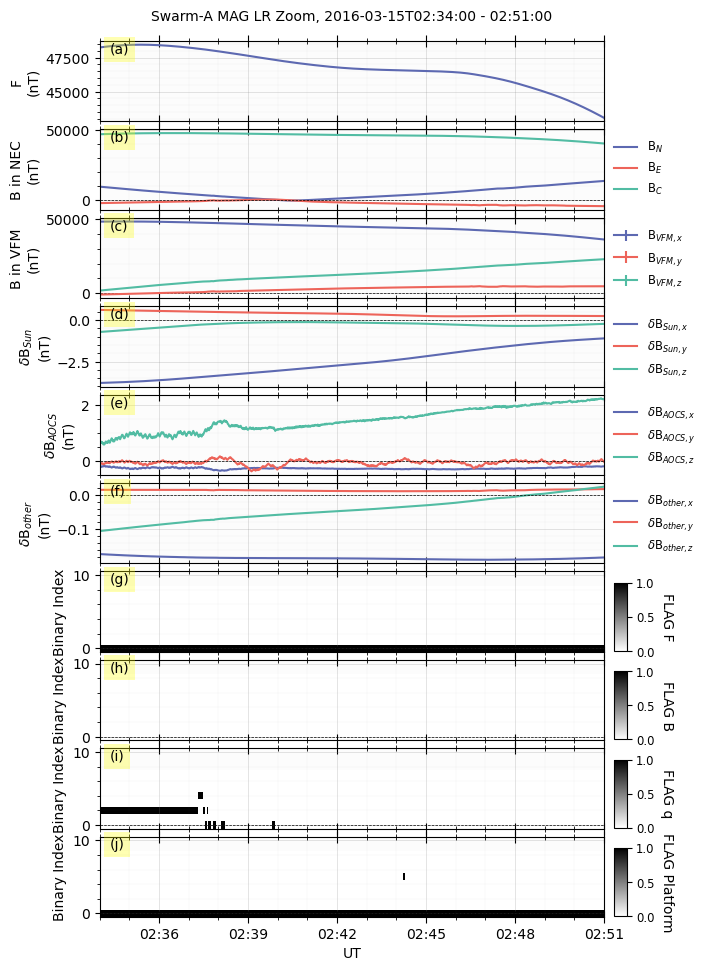
\includegraphics[width=0.7\linewidth]{files/580162baa01bb053b733a4b2044e8469.png}

The above figure shows different variables from the Swarm MAG LR products. The panel layouts can be changed flexibly.

For example, to remove the panels of ``F'' and flags, remove the first inner list \texttt{[ds['F']],}, \texttt{[ds['FLAG\_F\_BIN\_AUX']],}, \texttt{[ds['FLAG\_B\_BIN\_AUX']],}, \texttt{[ds['FLAG\_q\_BIN\_AUX']],}, and \texttt{[ds['FLAG\_Platform\_BIN\_AUX']],}.

Additionally, to remove one of the line plots (e.g., B\_VFM\_x) in panel c, change \texttt{[ds['B\_VFM\_x'], ds['B\_VFM\_y'], ds['B\_VFM\_z']],} to \texttt{[ds['B\_VFM\_y'], ds['B\_VFM\_z']],}.

\begin{verbatim}
fig = gsl_mpl.create_figure(figsize=(8, 8))
db = gsl_mpl.dashboards.TSDashboard(figure=fig, dt_fr=dt_fr, dt_to=dt_to)
panel_layouts = [
    [ds['B_N'], ds['B_E'], ds['B_C']],
    [ds['B_VFM_y'], ds['B_VFM_z']],
    [ds['dB_Sun_VFM_y'], ds['dB_Sun_VFM_z']],
    [ds['dB_AOCS_VFM_x'], ds['dB_AOCS_VFM_y'], ds['dB_AOCS_VFM_z']],
    [ds['dB_other_VFM_x'], ds['dB_other_VFM_y'], ds['dB_other_VFM_z']],
]
db.set_layout(panel_layouts)
# Plotting the data in the dashboard
db.draw()
# Add panel labels to the dashboard
db.add_panel_labels()
# Add a title to the dashboard
db.add_title(y=1.02,title='Swarm -{} MAG LR Zoom'.format(ds.sat_id), fontsize='medium', append_time=True)
# Show the figure/dashboard
db.show()
\end{verbatim}

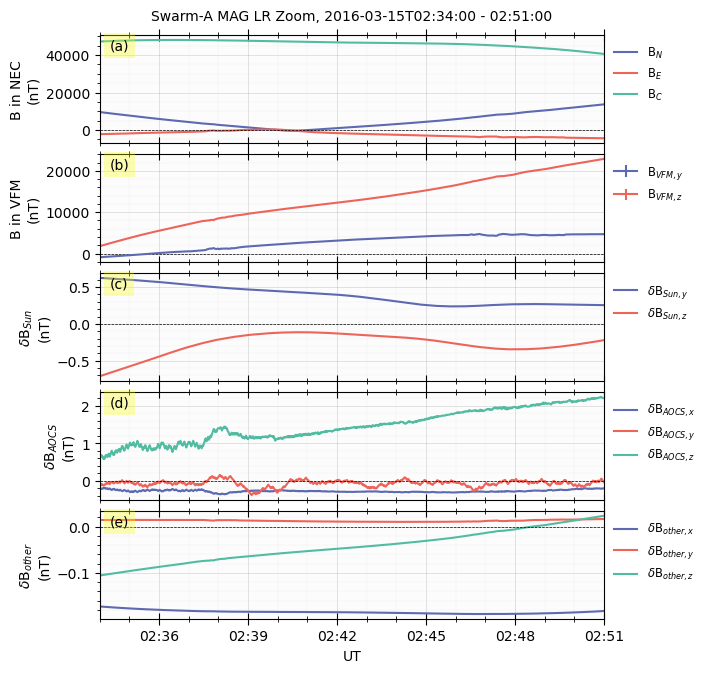
\includegraphics[width=0.7\linewidth]{files/85a0f316bd8769e9ab3d6f269e67400c.png}

\paragraph{Show satellite positions along the time axis}

GeospaceLAB \texttt{TSDashboard} is also able to show the satellite positions along the time axis by setting the keyword \texttt{timeline\_extra\_labels} when the dashboard object is created.

\begin{verbatim}
# Default kwargs for VirES data loading, which can be overridden when calling the dock method to load data from VirES. 
# The measurements, models, and residuals to load can be specified in the kwargs_products dictionary. 
# The default settings are for loading all available measurements and models, and no residuals. 
# The available measurements and models depend on the specific collection and product being loaded, 
# and can be checked in the VirES API documentation or by inspecting the variables in the loaded dataset.
kwargs_products_default = {
        "measurements": [
            'B_VFM', 'B_NEC', 'dB_Sun', 'dB_AOCS', 'dB_other', 'B_error',
            'q_NEC_CRF', 'Att_error',
            'Flags_B', 'Flags_q', 'Flags_Platform', 'Flags_F',
            'ASM_Freq_Dev', 'F', 'F_error', 'dF_Sun', 'dF_AOCS', 'dF_other',
        ],
        "models": [
            'CHAOS -Core',
        ],
        "residuals": True,
    }


db = gsl_mpl.dashboards.TSDashboard(
    dt_fr=dt_fr, dt_to=dt_to, figure_config={'figsize': (8, 5)},
    timeline_extra_labels=['GEO_LAT', 'GEO_LON', 'APEX_LAT', 'APEX_LON', 'APEX_MLT',] 
    )

ds_vires = db.dock(
    datasource_contents=['esa_eo', 'swarm', 'l1b', 'mag_lr'], 
    from_VirES=True, from_FAST=False,
    sat_id=sat_id, add_APEX=True,
    kwargs_VirES={"kwargs_products": kwargs_products_default},
)

panel_layouts = [
    [ds_vires['F_res_CHAOS -Core']],
    [ds_vires['B_res_CHAOS -Core_N'], ds_vires['B_res_CHAOS -Core_E'], ds_vires['B_res_CHAOS -Core_C']],
]

db.set_layout(panel_layouts=panel_layouts)
db.draw()
db.add_panel_labels()
db.add_title(title='Swarm -{} MAG LR Zoom from VirES OPER'.format(ds_vires.sat_id), fontsize='medium', append_time=True)
db.show()
\end{verbatim}

\begin{verbatim}
Create a new figure: Figure(800x500).
INFO: Loading data from VirES for collection SW_OPER_MAGA_LR_1B with products {'measurements': ['B_VFM', 'B_NEC', 'dB_Sun', 'dB_AOCS', 'dB_other', 'B_error', 'q_NEC_CRF', 'Att_error', 'Flags_B', 'Flags_q', 'Flags_Platform', 'Flags_F', 'ASM_Freq_Dev', 'F', 'F_error', 'dF_Sun', 'dF_AOCS', 'dF_other'], 'models': ['CHAOS -Core'], 'residuals': True}.
Processing:  100%|██████████|  [ Elapsed: 00:00, Remaining: 00:00 ] [1/1] 
Downloading: 100%|██████████|  [ Elapsed: 00:00, Remaining: 00:00 ] (0.322MB)
INFO: Data loaded from VirES.
WARNING: Variable name Spacecraft not found in the variable name dictionary, and no unique match found. Skipping this variable.
WARNING: Variable B_NEC_res_CHAOS -Core is not in the default variable names and does not match the patterns for automatically assigning configured variable names. It will be added without a configured variable name, and may not be included in the default panels for plotting and analysis. Please check if this variable should be included in the default variable names or if it follows the naming patterns for automatic assignment of configured variable names.
WARNING: Variable SC_GEO_R is not in the default variable names and does not match the patterns for automatically assigning configured variable names. It will be added without a configured variable name, and may not be included in the default panels for plotting and analysis. Please check if this variable should be included in the default variable names or if it follows the naming patterns for automatic assignment of configured variable names.
/opt/anaconda3/envs/Swarm/lib/python3.12/site -packages/numpy/_core/numeric.py:442: RuntimeWarning: invalid value encountered in cast
  multiarray.copyto(res, fill_value, casting='unsafe')
\end{verbatim}

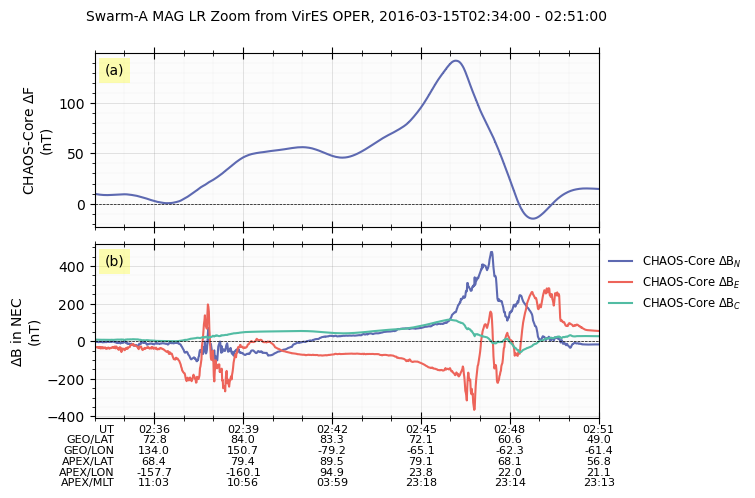
\includegraphics[width=0.7\linewidth]{files/f313b5264ef8b7d4fc31eca40c3dc88f.png}

\paragraph{Combined time-series plots from multiple datasets}

The following script show the figure combining data from three Swarm datasets, including

\begin{itemize}
\item B in NEC coordinates in Swarm MAG LR,
\item disturbed B in NEC from Swarm MAG LR from Swarm VirES,
\item the field-aligned current from Swarm FAC LLS,
\item and the ion velocities from Swarm EFI TCT02 data.
\end{itemize}

\begin{verbatim}
fig = gsl_mpl.create_figure(figsize=(8, 8))
db = gsl_mpl.dashboards.TSDashboard(
    figure=fig, dt_fr=dt_fr, dt_to=dt_to,
    timeline_extra_labels=['GEO_LAT', 'GEO_LON', 'APEX_LAT', 'APEX_LON', 'APEX_MLT',] 
    )
ds_mag = db.dock(
    datasource_contents=['esa_eo', 'swarm', 'l1b', 'mag_lr'], 
    sat_id=sat_id, 
    add_APEX=True,)
ds_vires = db.dock(
    datasource_contents=['esa_eo', 'swarm', 'l1b', 'mag_lr'], 
    from_VirES=True, from_FAST=False,
    sat_id=sat_id, add_APEX=True,
    kwargs_VirES={"kwargs_products": kwargs_products_default},
)
ds_FAC = db.dock(
    datasource_contents=['esa_eo', 'swarm', 'l2daily', 'fac_lls_dual'], 
    add_APEX=True,) # sat_id is fixed to 'AC' for LLS Dual product

ds_tct02 = db.dock(
    datasource_contents=['esa_eo', 'swarm', 'advanced', 'efi_tct02'], 
    sat_id=sat_id, add_APEX=True,
)

panel_layouts = [
    [ds_mag['B_N'], ds_mag['B_E'], ds_mag['B_C']],
    [ds_vires['B_res_CHAOS -Core_N'], ds_vires['B_res_CHAOS -Core_E'], ds_vires['B_res_CHAOS -Core_C']],
    [ds_FAC['j_FA']],
    [ds_tct02['v_i_H_x'], ds_tct02['v_i_V_x'], ds_tct02['v_i_H_y'], ds_tct02['v_i_V_z']],
]
db.set_layout(panel_layouts)
# Plotting the data in the dashboard
db.draw()
# Add panel labels to the dashboard
db.add_panel_labels()
# Add a title to the dashboard
db.add_title(y=1.02,title='Swarm -{} MAG LR Zoom'.format(ds.sat_id), fontsize='medium', append_time=True)
# Show the figure/dashboard
db.show()
\end{verbatim}

\begin{verbatim}
Searching the data product "MAG_LR" with the version "latest" on the server...
The file [PosixPath('/data/afys -ionosphere/data/ESA/SWARM/Level1b/MAG_LR/0701/Sat_A/2016/SW_OPER_MAGA_LR_1B_20160315T000000_20160315T235959_0701_MDR_MAG_LR.cdf'), PosixPath('/data/afys -ionosphere/data/ESA/SWARM/Level1b/MAG_LR/0701/Sat_A/2016/SW_OPER_MAGA_LR_1B_20160315T000000_20160315T235959_0701_ASM_VFM_IC.cdf')] already exists: skip downloading.
WARNING: Multiple files found for the pattern *20160315T000000*20160315T235959*0701*.cdf in the directory /data/afys -ionosphere/data/ESA/SWARM/Level1b/MAG_LR/0701/Sat_A/2016!
INFO: Loading data from VirES for collection SW_OPER_MAGA_LR_1B with products {'measurements': ['B_VFM', 'B_NEC', 'dB_Sun', 'dB_AOCS', 'dB_other', 'B_error', 'q_NEC_CRF', 'Att_error', 'Flags_B', 'Flags_q', 'Flags_Platform', 'Flags_F', 'ASM_Freq_Dev', 'F', 'F_error', 'dF_Sun', 'dF_AOCS', 'dF_other'], 'models': ['CHAOS -Core'], 'residuals': True}.
Processing:  100%|██████████|  [ Elapsed: 00:01, Remaining: 00:00 ] [1/1] 
Downloading: 100%|██████████|  [ Elapsed: 00:00, Remaining: 00:00 ] (0.322MB)
INFO: Data loaded from VirES.
WARNING: Variable name Spacecraft not found in the variable name dictionary, and no unique match found. Skipping this variable.
WARNING: Variable B_NEC_res_CHAOS -Core is not in the default variable names and does not match the patterns for automatically assigning configured variable names. It will be added without a configured variable name, and may not be included in the default panels for plotting and analysis. Please check if this variable should be included in the default variable names or if it follows the naming patterns for automatic assignment of configured variable names.
WARNING: Variable SC_GEO_R is not in the default variable names and does not match the patterns for automatically assigning configured variable names. It will be added without a configured variable name, and may not be included in the default panels for plotting and analysis. Please check if this variable should be included in the default variable names or if it follows the naming patterns for automatic assignment of configured variable names.
/opt/anaconda3/envs/Swarm/lib/python3.12/site -packages/numpy/_core/numeric.py:442: RuntimeWarning: invalid value encountered in cast
  multiarray.copyto(res, fill_value, casting='unsafe')
Searching the data product "FAC_LLS_DUAL" with the version "latest" on the server...
The file [PosixPath('/data/afys -ionosphere/data/ESA/SWARM/Level2daily/FAC_LLS_DUAL/0101/Sat_AC/2016/SW_OPER_FAC_LLS_2F_20160315T000000_20160315T235959_0101.cdf')] already exists: skip downloading.
Searching the data product "EFI_TCT02" with the version "latest" on the server...
The file [PosixPath('/data/afys -ionosphere/data/ESA/SWARM/Advanced/EFI_TII/TCT02/0401/Sat_A/2016/SW_EXPT_EFIA_TCT02_20160315T002346_20160315T130037_0401.cdf')] already exists: skip downloading.
\end{verbatim}

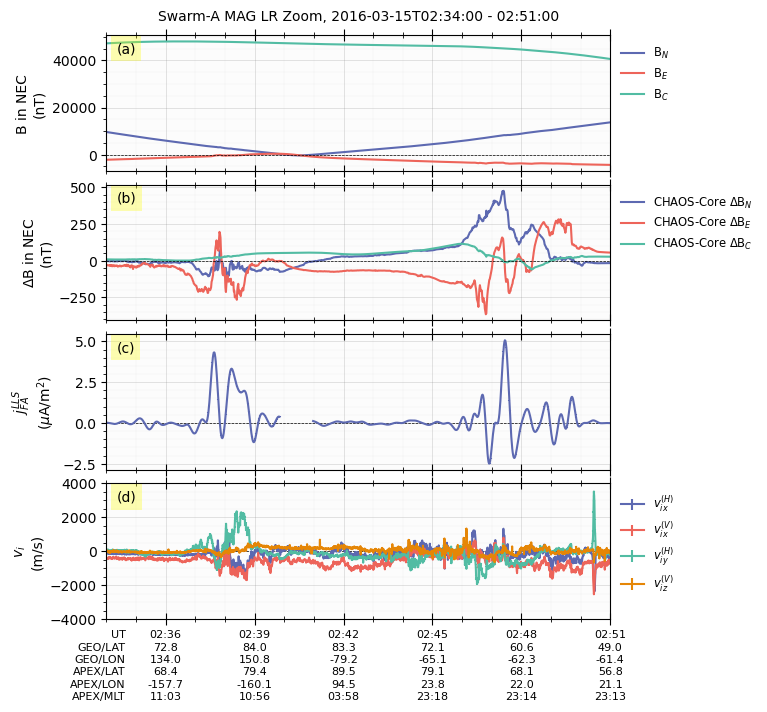
\includegraphics[width=0.7\linewidth]{files/06ef45a92cda4380178fc24ffb4e3238.png}

\subsubsection{Polar maps}

The along-track data can be also plotted in polar maps in GeospaceLAB using \texttt{GeoDashboard}.

\paragraph{Satellite trajectory}

\begin{verbatim}
# Create a geodashboard object
db = gsl_mpl.geomap.geodashboards.GeoDashboard(dt_fr=dt_fr, dt_to=dt_to, figure_config={'figsize': (5, 5)})
# Set the layout of the geodashboard to have one panel that will display the satellite's trajectory on a map
db.set_layout(1, 1)     # Set the layout to have 1 row and 1 column, meaning there will be one panel in the geodashboard
# Add a polar map panel
time_c = dt_fr + (dt_to - dt_fr) / 2
panel = db.add_polar_map(
        row_ind=0, 
        col_ind=0, 
        style='mlt -fixed',  # 'glon -fixed', 'lst -fixed', or 'mlt -fixed'
        cs='APEX',
        mlt_c=0., 
        pole='N',   # 'N' for North Pole, 'S' for South Pole
        ut=time_c,  # The time when the satellite is close tot the pole, 
                    # used for calculating the magnetic coordinates and plotting the satellite trajectory on the polar map.
        boundary_lat=60., # The latitude of the boundary of the polar map. 
        mirror_south=True # Applicable when pole = 'S'
    )
# Add grids and labels to the polar map
panel.overlay_gridlines(lat_label_clock=2.2)
panel.overlay_coastlines()
# Show the satellite trajectory on the polar map using the coordinates from the ds_mag dataset
sc_dts = ds_mag['SC_DATETIME'].flatten()
sc_glats = ds_mag['SC_GEO_LAT'].flatten()
sc_glons = ds_mag['SC_GEO_LON'].flatten()
sc_alts = (ds_mag['SC_GEO_r'].flatten() - 1) * 6371.2  # Convert from Earth radii to km
sc_coords = {'lat': sc_glats, 'lon': sc_glons, 'height': sc_alts}

# Overlay the satellite trajectory with ticks
panel.overlay_sc_trajectory(
    sc_ut=sc_dts, 
    sc_coords=sc_coords, 
    cs='GEO', # Input coordinate system
    color='darkblue',
    time_tick = True, 
    time_tick_res=300., 
    time_tick_scale=0.05,
    time_tick_label=True, 
    time_tick_label_format="%H:%M", 
    time_tick_label_fontsize=8,
    time_tick_label_rotation=45., 
    time_tick_label_offset=0.05, 
    time_tick_label_fontweight='normal',
    time_minor_tick=True, 
    time_minor_tick_res=60,
    show_start_point=True,
    )
\end{verbatim}

\begin{verbatim}
Create a new figure: Figure(500x500).
/opt/anaconda3/envs/Swarm/lib/python3.12/site -packages/apexpy/apex.py:556: RuntimeWarning: invalid value encountered in <lambda> (vectorized)
  alat, alon = self._geo2apex(glat, glon, height)
/opt/anaconda3/envs/Swarm/lib/python3.12/site -packages/apexpy/apex.py:559: UserWarning: Apex latitude set to NaN where undefined (apex height may be < reference height)
  warnings.warn(''.join(['Apex latitude set to NaN where undefined ',
/opt/anaconda3/envs/Swarm/lib/python3.12/site -packages/shapely/creation.py:218: RuntimeWarning: invalid value encountered in linestrings
  return lib.linestrings(coords, np.intc(handle_nan), out=out, **kwargs)
\end{verbatim}

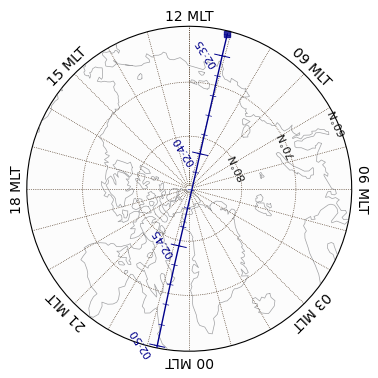
\includegraphics[width=0.7\linewidth]{files/6cea1f5b9e5b950995690dc60ffb2ced.png}

\paragraph{Along-track data in multicolored line}

\begin{verbatim}
# Create a geodashboard object
db = gsl_mpl.geomap.geodashboards.GeoDashboard(dt_fr=dt_fr, dt_to=dt_to, figure_config={'figsize': (5, 5)})
# Set the layout of the geodashboard to have one panel that will display the satellite's trajectory on a map
db.set_layout(1, 1)     # Set the layout to have 1 row and 1 column, meaning there will be one panel in the geodashboard
# Add a polar map panel
time_c = dt_fr + (dt_to - dt_fr) / 2
panel = db.add_polar_map(
        row_ind=0, 
        col_ind=0, 
        style='mlt -fixed',  # 'glon -fixed', 'lst -fixed', or 'mlt -fixed'
        cs='APEX',
        mlt_c=0., 
        pole='N',   # 'N' for North Pole, 'S' for South Pole
        ut=time_c,  # The time when the satellite is close tot the pole, 
                    # used for calculating the magnetic coordinates and plotting the satellite trajectory on the polar map.
        boundary_lat=60., # The latitude of the boundary of the polar map. 
        mirror_south=True # Applicable when pole = 'S'
    )
# Add grids and labels to the polar map
panel.overlay_gridlines(lat_label_clock=2.2)
panel.overlay_coastlines()
# Show the satellite trajectory on the polar map using the coordinates from the ds_mag dataset
sc_dts = ds_FAC['SC_DATETIME'].flatten()
sc_glats = ds_FAC['SC_GEO_LAT'].flatten()
sc_glons = ds_FAC['SC_GEO_LON'].flatten()
sc_alts = (ds_FAC['SC_GEO_r'].flatten() - 1) * 6371.2  # Convert from Earth radii to km
sc_coords = {'lat': sc_glats, 'lon': sc_glons, 'height': sc_alts}

# Get the FAC data from the ds_FAC dataset, which will be used for coloring the satellite trajectory on the polar map.
j_FA = ds_FAC['j_FA'].flatten()
# Overlay the FAC data on the satellite trajectory by passing it as the color argument in the overlay_sc_trajectory method.
icl = panel.overlay_sc_coloured_line(
    j_FA,
    sc_ut=sc_dts, 
    sc_coords=sc_coords, 
    cs='GEO', # Input coordinate system
    c_map = 'turbo',
    c_lim = [ -4, 4],   
)
panel.add_colorbar(icl, c_label=r'j$_{FA}$ (µA/m$^2$)',)

# Overlay the satellite trajectory with ticks
panel.overlay_sc_trajectory(
    sc_ut=sc_dts, 
    sc_coords=sc_coords, 
    cs='GEO', # Input coordinate system
    color='gray',
    time_tick = True, 
    time_tick_res=300., 
    time_tick_scale=0.05,
    time_tick_label=True, 
    time_tick_label_format="%H:%M", 
    time_tick_label_fontsize=8,
    time_tick_label_rotation=90., 
    time_tick_label_offset=0.1, 
    time_tick_label_fontweight='normal',
    time_minor_tick=True, 
    time_minor_tick_res=60,
    show_start_point=True,
    )
\end{verbatim}

\begin{verbatim}
Create a new figure: Figure(500x500).
/opt/anaconda3/envs/Swarm/lib/python3.12/site -packages/apexpy/apex.py:556: RuntimeWarning: invalid value encountered in <lambda> (vectorized)
  alat, alon = self._geo2apex(glat, glon, height)
/opt/anaconda3/envs/Swarm/lib/python3.12/site -packages/apexpy/apex.py:559: UserWarning: Apex latitude set to NaN where undefined (apex height may be < reference height)
  warnings.warn(''.join(['Apex latitude set to NaN where undefined ',
/opt/anaconda3/envs/Swarm/lib/python3.12/site -packages/shapely/creation.py:218: RuntimeWarning: invalid value encountered in linestrings
  return lib.linestrings(coords, np.intc(handle_nan), out=out, **kwargs)
\end{verbatim}

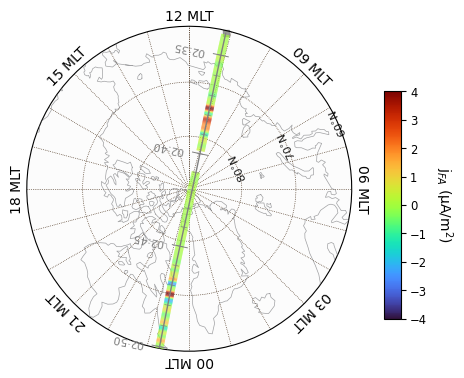
\includegraphics[width=0.7\linewidth]{files/462512135a4968f368c03dd1b612a6f7.png}

\paragraph{Cross-track vectors}

\begin{verbatim}
# Create a geodashboard object
db = gsl_mpl.geomap.geodashboards.GeoDashboard(dt_fr=dt_fr, dt_to=dt_to, figure_config={'figsize': (5, 5)})
# Set the layout of the geodashboard to have one panel that will display the satellite's trajectory on a map
db.set_layout(1, 1)     # Set the layout to have 1 row and 1 column, meaning there will be one panel in the geodashboard
# Add a polar map panel
time_c = dt_fr + (dt_to - dt_fr) / 2
panel = db.add_polar_map(
        row_ind=0, 
        col_ind=0, 
        style='mlt -fixed',  # 'glon -fixed', 'lst -fixed', or 'mlt -fixed'
        cs='APEX',
        mlt_c=0., 
        pole='N',   # 'N' for North Pole, 'S' for South Pole
        ut=time_c,  # The time when the satellite is close tot the pole, 
                    # used for calculating the magnetic coordinates and plotting the satellite trajectory on the polar map.
        boundary_lat=60., # The latitude of the boundary of the polar map. 
        mirror_south=True # Applicable when pole = 'S'
    )
# Add grids and labels to the polar map
panel.overlay_gridlines(lat_label_clock=2.2)
panel.overlay_coastlines()
# Show the satellite trajectory on the polar map using the coordinates from the ds_mag dataset
sc_dts = ds_tct02['SC_DATETIME'].flatten()
sc_glats = ds_tct02['SC_GEO_LAT'].flatten()
sc_glons = ds_tct02['SC_GEO_LON'].flatten()
sc_alts = (ds_tct02['SC_GEO_r'].flatten() - 1) * 6371.2  # Convert from Earth radii to km
sc_coords = {'lat': sc_glats, 'lon': sc_glons, 'height': sc_alts}

# Get the cross -track ion velocity data from the ds_tct02 dataset, which will be used for coloring the satellite trajectory on the polar map.
v_i_H_y = ds_tct02['v_i_H_y'].flatten()
# Overlay the cross -track ion velocity data on the satellite trajectory by passing it as the color argument in the overlay_sc_trajectory method.
panel.overlay_cross_track_vector(
        vector= -v_i_H_y.flatten(), unit_vector=1000, vector_unit='m/s', alpha=1, color='c', vector_width=1, 
        sc_coords=sc_coords, sc_ut=sc_dts, cs='GEO', shading='on', legend_pos_x=0.9, legend_pos_y=1
    )

# Overlay the satellite trajectory with ticks
panel.overlay_sc_trajectory(
    sc_ut=sc_dts, 
    sc_coords=sc_coords, 
    cs='GEO', # Input coordinate system
    color='gray',
    time_tick = True, 
    time_tick_res=300., 
    time_tick_scale=0.05,
    time_tick_label=True, 
    time_tick_label_format="%H:%M", 
    time_tick_label_fontsize=8,
    time_tick_label_rotation=90., 
    time_tick_label_offset=0.1, 
    time_tick_label_fontweight='normal',
    time_minor_tick=True, 
    time_minor_tick_res=60,
    show_start_point=True,
    )
\end{verbatim}

\begin{verbatim}
Create a new figure: Figure(500x500).
/opt/anaconda3/envs/Swarm/lib/python3.12/site -packages/apexpy/apex.py:556: RuntimeWarning: invalid value encountered in <lambda> (vectorized)
  alat, alon = self._geo2apex(glat, glon, height)
/opt/anaconda3/envs/Swarm/lib/python3.12/site -packages/apexpy/apex.py:559: UserWarning: Apex latitude set to NaN where undefined (apex height may be < reference height)
  warnings.warn(''.join(['Apex latitude set to NaN where undefined ',
/opt/anaconda3/envs/Swarm/lib/python3.12/site -packages/shapely/creation.py:218: RuntimeWarning: invalid value encountered in linestrings
  return lib.linestrings(coords, np.intc(handle_nan), out=out, **kwargs)
\end{verbatim}

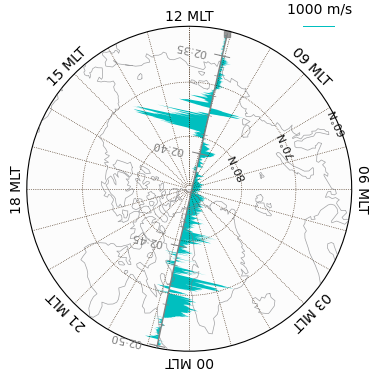
\includegraphics[width=0.7\linewidth]{files/83e7d2af9fe7313af172ccb227bbc51c.png}

\subsection{Data grouping and gridding for LEO satellite data}

GeospaceLAB provides tools for grouping and gridding data from Low Earth Orbit (LEO) satellites. This process is essential for analyzing and visualizing satellite data effectively. For the Swarm mission, the Swarm \texttt{Dataset} class has a built-in method (so called \texttt{gridding}) for grouping and gridding along-track data. The gridding method allows you to specify the orbit sector to be gridded, the grid resolution, and the type of interpolation/binning to be used.

The gridding results have been used in a recent study on the polar ionosphere-thermosphere coupling during the May 2024 superstorm  \citep{cai2026ionosphere}, to analyze the spatial distribution of ionospheric electron density, thermospheric neutral density and composition, and their relationship with geomagnetic activity.

\begin{framed}
\textbf{Note}\\
The gridding method is designed to work with the Swarm \texttt{Dataset} class, which is specifically tailored for handling Swarm satellite data. If you are working with data from other LEO satellites, you may need to implement a custom gridding approach or adapt the existing method to suit your needs.
\end{framed}

\begin{framed}
\textbf{Note}\\
The gridding method is applicable for along-track data, meaning that the data with support variables like ``SC\_DATETIME'' and ``SC\_GEO\_LAT''. Hence, this method is not suitable for several data products, such as Swarm AEJ PBS data, which do not have the necessary support variables for along-track gridding.
\end{framed}

\begin{verbatim}
import datetime
import matplotlib.pyplot as plt
import numpy as np
import pathlib

import geospacelab.visualization.mpl.dashboards as dashboards
\end{verbatim}

\subsubsection{Simple gridding example}

The following function demonstrates an example to call the gridding method for the Swarm DNS POD data product. In this example, we will grid the data in orbit sector of ascending phase with a specified grid resolution and interpolation method.

\begin{verbatim}
def simple_gridding_example():
    # Initialize the start and end datetime for the data to be gridded
    dt_fr = datetime.datetime(2024, 5, 10, 0, 0, 0)
    dt_to = datetime.datetime(2024, 5, 14, 0, 0, 0)
    sat_id = 'A'
    # Create a Dashboard object for visualizing the gridded data
    db = dashboards.TSDashboard(
        dt_fr = dt_fr,
        dt_to = dt_to,
        figure_config = {
            'figsize': (10, 8),
        }
    )
    ds_pod = db.dock(
        datasource_contents=['esa_eo', 'swarm', 'l2daily', 'dns_pod'], 
        sat_id=sat_id, 
        add_APEX=True, add_AACGM=True,
    )
    
    ds_sector_ASC = ds_pod.gridding(
        # Variable names to be gridded, 
        # which should be a subset of the variables in the original dataset. 
        # The gridded variables will be renamed with a prefix "SECTOR_ASC_GRID_" 
        # to distinguish them from the original variables, 
        # where ASC stands for Ascending.
        var_names_gridding=['rho_n', 'SC_GEO_ALT', 'SC_GEO_LAT', 'SC_GEO_LON'],
        # Sector to be gridded, which can be 'ASC' for ascending phase, 
        # 'DSC' for descending phase, 
        # 'N' for northern hemisphere, 
        # or 'S' for southern hemisphere.
        sector = 'ASC',
        # Coordinate system for the gridding, which can be 'GEO' for geographic coordinates,
        # 'APEX' for apex coordinates, or 'AACGM' for AACGM coordinates.
        sector_cs = 'GEO',
        # Latitude boundary for the sector to be gridded.
        boundary_lat = 90.,
        # Whether to perform along -track interpolation for the gridding.
        along_track_interp=True, 
        # Interpolation method for along -track interpolation, 
        # which can be 'linear' for linear interpolation.
        along_track_interp_method='linear',
        # Grid resolution along the x axis (time axis). 
        # If None, the grid resolution will be automatically determined based on 
        # the satellite orbital period.
        x_grid_res=None,
        # Grid resolution along the y axis (latitude axis) in degrees.
        y_grid_res=0.5,
        # Data resolution for the original data to be gridded. 
        # If None, the data resolution will be automatically determined 
        # based on the original data. For LEO satellite, the resolution is 
        # typically around 90 * 60 = 5400 s.
        x_data_res=None, 
        # Data resolution for the original data. For the POD data, 
        # the resolution is 30 s. 
        y_data_res=30, 
        # Scale factor for the data resolution along the y axis for better visualization.
        y_data_res_scale=1.5,
        visual='on',
    )
    grid_rho_n_ASC = ds_sector_ASC['SECTOR_ASC_GRID_rho_n']
    
    panel_layouts = [
        [ds_pod['rho_n']],
        [ds_pod['SC_GEO_LAT']],
        [ds_pod['SC_GEO_LST']],
        [grid_rho_n_ASC],
    ]
    
    # set axis scale and unit for better visualization, removing exponent for density in the upper -left corner of the panel.
    ds_pod['rho_n'].visual.axis[1].data_scale = 1e12 
    ds_pod['rho_n'].visual.axis[1].unit = r'$\cdot$10$^{ -12}$ kg$\cdot$m$^{ -3}$'
    
    grid_rho_n_ASC.visual.axis[2].data_scale = 1e12
    grid_rho_n_ASC.visual.axis[2].unit = r'$\cdot$10$^{ -12}$ kg$\cdot$m$^{ -3}$'
    # Set sector labels and data limits for better visualization
    grid_rho_n_ASC.visual.axis[2].lim = [0, 8]
    
    db.set_layout(panel_layouts=panel_layouts, left=0.25, right=0.86, top=0.9, bottom=0.06, hspace=0.2)
    db.draw()
    
    # Post -settings
    # Set panel and axis labels for sector panels
    # For Sector North panel
    ax = db.panels[3]()
    ds_sector_ASC.format_pseudo_lat_axis(ax, 'ASC', inverse=False, add_sperator=True)
    ds_sector_ASC.format_pseudo_lat_label(ax, 'ASC', y_tick_res=45)
    ax.set_ylabel('Ascending\n' + ax.get_ylabel(), labelpad=20)
    
    lsts_asc = ds_sector_ASC.ascending_nodes['GEO_LST']
    lsts_dsc = ds_sector_ASC.descending_nodes['GEO_LST']
    lst_median_asc = lsts_asc[len(lsts_asc) // 2]
    lst_median_dsc = lsts_dsc[len(lsts_dsc) // 2]
    
    db.add_title(
        y=1.03,
        title='Swarm -{} DNS/POD gridded in different orbit sectors \n'.format(ds_pod.sat_id) + \
            r'ASC: $\sim${:.1f} LST, DSC: $\sim${:.1f} LST'.format(lst_median_asc, lst_median_dsc),
        fontsize='large', append_time=False)
    db.show()
    
simple_gridding_example()
\end{verbatim}

\begin{verbatim}
Create a new figure: Figure(1000x800).
Searching the data product "DNS_POD" with the version "latest" on the server...
\end{verbatim}

\begin{verbatim}
The file [PosixPath('/data/afys -ionosphere/data/ESA/SWARM/Level2daily/DNS_POD/0301/Sat_A/2024/SW_OPER_DNSAPOD_2__20240510T000000_20240510T235930_0301.cdf')] already exists: skip downloading.
The file [PosixPath('/data/afys -ionosphere/data/ESA/SWARM/Level2daily/DNS_POD/0301/Sat_A/2024/SW_OPER_DNSAPOD_2__20240511T000000_20240511T235930_0301.cdf')] already exists: skip downloading.
The file [PosixPath('/data/afys -ionosphere/data/ESA/SWARM/Level2daily/DNS_POD/0301/Sat_A/2024/SW_OPER_DNSAPOD_2__20240512T000000_20240512T235930_0301.cdf')] already exists: skip downloading.
The file [PosixPath('/data/afys -ionosphere/data/ESA/SWARM/Level2daily/DNS_POD/0301/Sat_A/2024/SW_OPER_DNSAPOD_2__20240513T000000_20240513T235930_0301.cdf')] already exists: skip downloading.
The file [PosixPath('/data/afys -ionosphere/data/ESA/SWARM/Level2daily/DNS_POD/0301/Sat_A/2024/SW_OPER_DNSAPOD_2__20240514T000000_20240514T235930_0301.cdf')] already exists: skip downloading.
\end{verbatim}

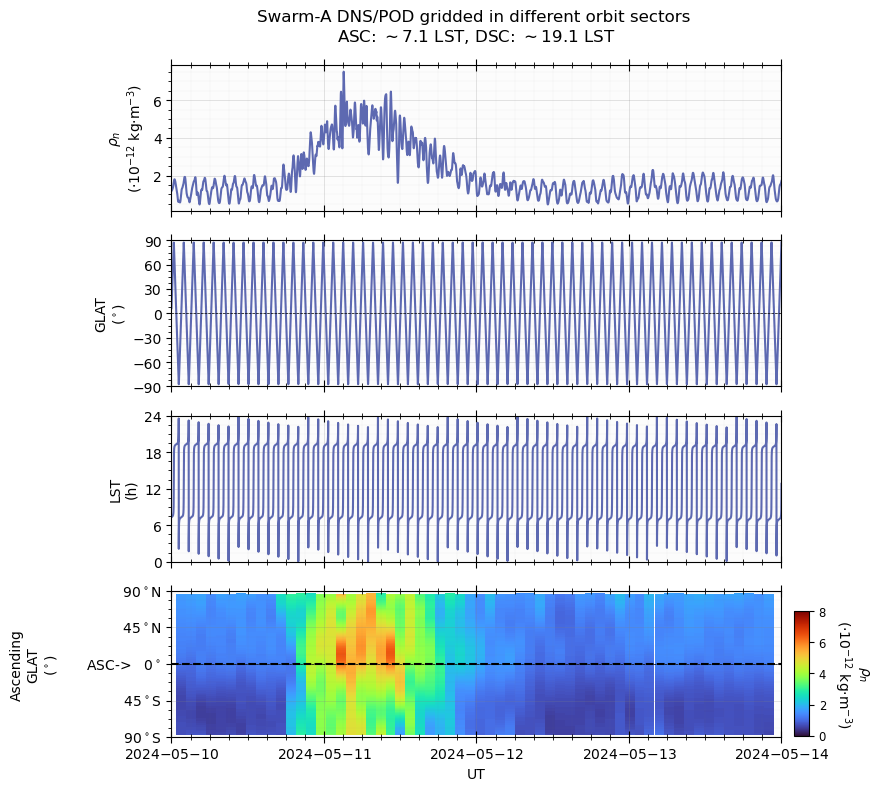
\includegraphics[width=0.7\linewidth]{files/71970e57797d0f91ac553c23041b6998.png}

\subsubsection{Gridding data in multiple orbit sectors}

The following function demonstrates an example to call the gridding method for the Swarm DNS POD data product in multiple orbit sectors, including

\begin{itemize}
\item N: Northern hemisphere,
\item S: Southern hemisphere,
\item ASC: ascending phase,
\item DSC: descending phase.
\end{itemize}

In this example, we will grid the data in the four sectors with the same grid resolution and interpolation method, and then visualize the gridded results together for comparison.

\begin{verbatim}
def test_gridding_interpolation_DNS_POD():
    """Test Swarm DNS/POD data product
    
    """
    dt_fr = datetime.datetime(2024, 5, 10, 0, 0)
    dt_to = datetime.datetime(2024, 5, 14, 0, 0)

    db = dashboards.TSDashboard(
        dt_fr=dt_fr, dt_to=dt_to, figure_config={'figsize': (10, 10)},
        )

    ds = db.dock(datasource_contents=['esa_eo', 'swarm', 'l2daily', 'dns_pod'], sat_id='A', add_APEX=True, add_AACGM=True)
    
    ds_sector_N = ds.gridding(
        var_names_gridding=['rho_n', 'SC_GEO_ALT', 'SC_GEO_LAT', 'SC_GEO_LON'],
        sector = 'N',
        sector_cs = 'GEO',
        boundary_lat = 0.,
        along_track_interp=True, along_track_interp_method='linear',
        x_grid_res=None,
        y_grid_res=0.5,
        x_data_res=None, 
        y_data_res=30, 
        y_data_res_scale=1.5,
        visual='on',
    )
    
    ds_sector_S = ds.gridding(
        var_names_gridding=['rho_n', 'SC_GEO_ALT', 'SC_GEO_LAT', 'SC_GEO_LON'],
        sector = 'S',
        sector_cs = 'GEO',
        boundary_lat = 0.,
        along_track_interp=True, along_track_interp_method='linear',
        x_grid_res=None,
        y_grid_res=0.5,
        x_data_res=None, 
        y_data_res=30, 
        y_data_res_scale=1.5,
        visual='on',
    )
    
    ds_sector_ASC = ds.gridding(
        var_names_gridding=['rho_n', 'SC_GEO_ALT', 'SC_GEO_LAT', 'SC_GEO_LON'],
        sector = 'ASC',
        sector_cs = 'GEO',
        boundary_lat = 90.,
        along_track_interp=True, along_track_interp_method='linear',
        x_grid_res=None,
        y_grid_res=0.5,
        x_data_res=None, 
        y_data_res=30, 
        y_data_res_scale=1.5,
        visual='on',
    )
    
    ds_sector_DSC = ds.gridding(
        var_names_gridding=['rho_n', 'SC_GEO_ALT', 'SC_GEO_LAT', 'SC_GEO_LON'],
        sector = 'DSC',
        sector_cs = 'GEO',
        boundary_lat = 90.,
        along_track_interp=True, along_track_interp_method='linear',
        x_grid_res=None,
        y_grid_res=0.5,
        x_data_res=None, 
        y_data_res=30, 
        y_data_res_scale=1.5,
        visual='on',
    )
    
    grid_rho_n_N = ds_sector_N['SECTOR_N_GRID_rho_n']
    grid_rho_n_S = ds_sector_S['SECTOR_S_GRID_rho_n']
    grid_rho_n_ASC = ds_sector_ASC['SECTOR_ASC_GRID_rho_n']
    grid_rho_n_DSC = ds_sector_DSC['SECTOR_DSC_GRID_rho_n']
    
    panel_layouts = [
        [ds['rho_n']],
        [ds['SC_GEO_LAT']],
        # [ds['SC_GEO_LON']],
        # [ds['SC_GEO_LST']],
        [grid_rho_n_N],
        [grid_rho_n_S],
        [grid_rho_n_ASC],
        [grid_rho_n_DSC],
    ]
    
    # set axis scale and unit for better visualization, removing exponent for density in the upper -left corner of the panel.
    ds['rho_n'].visual.axis[1].data_scale = 1e12 
    ds['rho_n'].visual.axis[1].unit = r'$\cdot$10$^{ -12}$ kg$\cdot$m$^{ -3}$'
    
    grid_rho_n_N.visual.axis[2].data_scale = 1e12
    grid_rho_n_N.visual.axis[2].unit = r'$\cdot$10$^{ -12}$ kg$\cdot$m$^{ -3}$'
    grid_rho_n_S.visual.axis[2].data_scale = 1e12
    grid_rho_n_S.visual.axis[2].unit = r'$\cdot$10$^{ -12}$ kg$\cdot$m$^{ -3}$'
    grid_rho_n_ASC.visual.axis[2].data_scale = 1e12
    grid_rho_n_ASC.visual.axis[2].unit = r'$\cdot$10$^{ -12}$ kg$\cdot$m$^{ -3}$'
    grid_rho_n_DSC.visual.axis[2].data_scale = 1e12
    grid_rho_n_DSC.visual.axis[2].unit = r'$\cdot$10$^{ -12}$ kg$\cdot$m$^{ -3}$'
    
    # Set sector labels and data limits
    grid_rho_n_N.visual.axis[2].lim = [0, 8]
    grid_rho_n_S.visual.axis[2].lim = [0, 8]
    grid_rho_n_ASC.visual.axis[2].lim = [0, 8]
    grid_rho_n_DSC.visual.axis[2].lim = [0, 8]
    
    db.set_layout(panel_layouts=panel_layouts, left=0.25, right=0.86, top=0.93, bottom=0.06, hspace=0.3)
    db.draw()
    
    # Post -settings
    # Set panel and axis labels for sector panels
    # For Sector North panel
    ax = db.panels[2]()
    ds_sector_N.format_pseudo_lat_axis(ax, 'N', inverse=False, add_sperator=True)
    ds_sector_N.format_pseudo_lat_label(ax, 'N', y_tick_res=45)
    ax.set_ylabel('Northern Hemi.\n' + ax.get_ylabel(), labelpad=20)
    ax = db.panels[3]()
    ds_sector_S.format_pseudo_lat_axis(ax, 'S', inverse=False, add_sperator=True)
    ds_sector_S.format_pseudo_lat_label(ax, 'S', y_tick_res=45)
    ax.set_ylabel('Southern Hemi.\n' + ax.get_ylabel(), labelpad=20)
    ax = db.panels[4]()
    ds_sector_ASC.format_pseudo_lat_axis(ax, 'ASC', inverse=False, add_sperator=True)
    ds_sector_ASC.format_pseudo_lat_label(ax, 'ASC', y_tick_res=45)
    ax.set_ylabel('Ascending\n' + ax.get_ylabel(), labelpad=20)
    ax = db.panels[5]()
    ds_sector_DSC.format_pseudo_lat_axis(ax, 'DSC', inverse=True, add_sperator=True)
    ds_sector_DSC.format_pseudo_lat_label(ax, 'DSC', y_tick_res=45)
    ax.set_ylabel('Descending\n' + ax.get_ylabel(), labelpad=20)
    
    lsts_asc = ds_sector_N.ascending_nodes['GEO_LST']
    lsts_dsc = ds_sector_N.descending_nodes['GEO_LST']
    lst_median_asc = lsts_asc[len(lsts_asc) // 2]
    lst_median_dsc = lsts_dsc[len(lsts_dsc) // 2]
    
    db.add_title(
        y=1.03,
        title='Swarm -{} DNS/POD gridded in different orbit sectors \n'.format(ds.sat_id) + \
            r'ASC: $\sim${:.1f} LST, DSC: $\sim${:.1f} LST'.format(lst_median_asc, lst_median_dsc),
        fontsize='large', append_time=False)
    
    return db
db = test_gridding_interpolation_DNS_POD()
db.show()
\end{verbatim}

\begin{verbatim}
Create a new figure: Figure(1000x1000).
Searching the data product "DNS_POD" with the version "latest" on the server...
\end{verbatim}

\begin{verbatim}
The file [PosixPath('/data/afys -ionosphere/data/ESA/SWARM/Level2daily/DNS_POD/0301/Sat_A/2024/SW_OPER_DNSAPOD_2__20240510T000000_20240510T235930_0301.cdf')] already exists: skip downloading.
The file [PosixPath('/data/afys -ionosphere/data/ESA/SWARM/Level2daily/DNS_POD/0301/Sat_A/2024/SW_OPER_DNSAPOD_2__20240511T000000_20240511T235930_0301.cdf')] already exists: skip downloading.
The file [PosixPath('/data/afys -ionosphere/data/ESA/SWARM/Level2daily/DNS_POD/0301/Sat_A/2024/SW_OPER_DNSAPOD_2__20240512T000000_20240512T235930_0301.cdf')] already exists: skip downloading.
The file [PosixPath('/data/afys -ionosphere/data/ESA/SWARM/Level2daily/DNS_POD/0301/Sat_A/2024/SW_OPER_DNSAPOD_2__20240513T000000_20240513T235930_0301.cdf')] already exists: skip downloading.
The file [PosixPath('/data/afys -ionosphere/data/ESA/SWARM/Level2daily/DNS_POD/0301/Sat_A/2024/SW_OPER_DNSAPOD_2__20240514T000000_20240514T235930_0301.cdf')] already exists: skip downloading.
\end{verbatim}

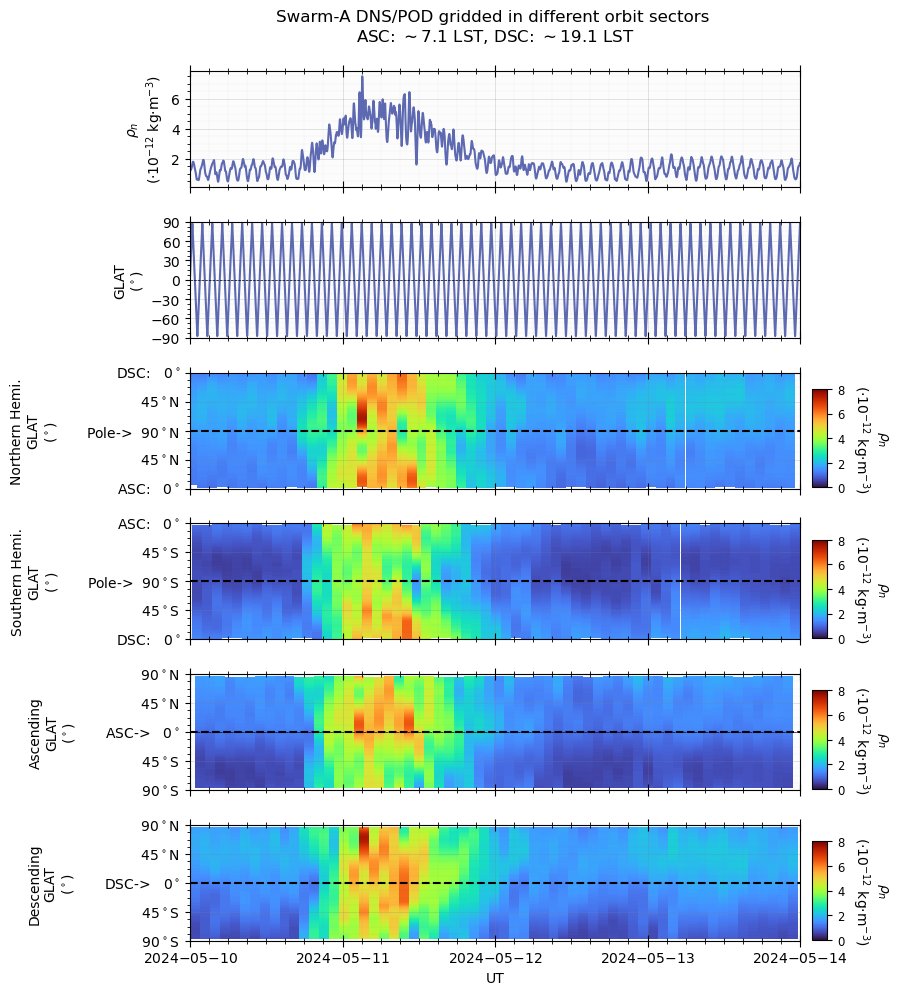
\includegraphics[width=0.7\linewidth]{files/de79ed0ebde25e6904777b2ea34a7e53.png}

\subsubsection{Gridding data by binning instead of interpolation}

Above examples use interpolation for gridding. Interpolation is useful when the data points are sparse or unevenly distributed, as it estimates values between known data points. The gridding method also supports binning the data with high time resolution, however, only large temporal scale structures need to be captured. The following function demonstrates how to use binning for gridding the Swarm FAC (1-s) data in the Northern hemispheric sector, and then visualize the results.

In addition, the gridding method also supports interpolating/binning the data with geomagnetic coordinate system, such as APEX, which is commonly used for ionospheric data analysis. The following function demonstrates how to use the gridding method to interpolate the Swarm FAC data in the Northern hemispheric sector with APEX coordinates, and then visualize the results.

\begin{verbatim}
def test_gridding_binning_FAC_TMS():
    """Test Swarm FAC TMS data product
    
    """
    dt_fr = datetime.datetime(2024, 5, 10, 0, 0)
    dt_to = datetime.datetime(2024, 5, 14, 0, 0)

    db = dashboards.TSDashboard(
        dt_fr=dt_fr, dt_to=dt_to, figure_config={'figsize': (10, 10)},
    )

    # ds_tms_dual = db.dock(datasource_contents=['esa_eo', 'swarm', 'l2daily', 'fac_tms_dual'], add_APEX=True,)
    
    ds_tms = db.dock(datasource_contents=['esa_eo', 'swarm', 'l2daily', 'fac_tms'], sat_id='A', add_APEX=True,)
   
    # Grid the data in the Northern hemispheric sector 
    # with geographic coordinates, using binning method for gridding.
    ds_sector_N = ds_tms.gridding(
        var_names_gridding=['j_FA',],
        sector = 'N',
        sector_cs = 'GEO',
        boundary_lat = 30.,
        along_track_binning=True, along_track_interp=False,
        along_track_binning_method='mean',
        along_track_binning_step=0.5,
        along_track_binning_res=2.5,
        x_grid_res=None,
        y_grid_res=2,
        x_data_res=None, 
        y_data_res=1, 
        y_data_res_scale=1.5,
        visual='on',
    )
    # Grid the data in the Northern hemispheric sector 
    # with APEX coordinates, using the same binning method for gridding.
    ds_sector_N_APEX = ds_tms.gridding(
        var_names_gridding=['j_FA',],
        sector = 'N',
        sector_cs = 'APEX',
        boundary_lat = 30.,
        along_track_binning=True, along_track_interp=False,
        along_track_binning_method='mean',
        along_track_binning_step=0.5,
        along_track_binning_res=2.5,
        x_grid_res=None,
        y_grid_res=2,
        x_data_res=None, 
        y_data_res=1, 
        y_data_res_scale=1.5,
        visual='on',
    )
    
    j_FA_N = ds_sector_N['SECTOR_N_GRID_j_FA']
    j_FA_N_APEX = ds_sector_N_APEX['SECTOR_N_GRID_j_FA']
    
    panel_layouts = [
        [ds_tms['j_FA']],
        [ds_tms['SC_GEO_LAT']],
        [j_FA_N,],
        [j_FA_N_APEX,],
    ]
    
    j_FA_N.visual.axis[2].lim = [ -2, 2]
    j_FA_N_APEX.visual.axis[2].lim = [ -2, 2]
    

    db.set_layout(panel_layouts=panel_layouts, left=0.25, right=0.86, top=0.93, bottom=0.06, hspace=0.2)
    db.draw()
    
    ax = db.panels[2]()
    ds_sector_N.format_pseudo_lat_axis(ax, 'N', inverse=False, add_sperator=True)
    ds_sector_N.format_pseudo_lat_label(ax, 'N', y_tick_res=45)
    ax.set_ylabel('Northern Hemi.\n' + ax.get_ylabel(), labelpad=20)
    ax = db.panels[3]()
    ds_sector_N_APEX.format_pseudo_lat_axis(ax, 'N', inverse=False, add_sperator=True)
    ds_sector_N_APEX.format_pseudo_lat_label(ax, 'N', y_tick_res=45)
    ax.set_ylabel('Northern Hemi.\n' + ax.get_ylabel(), labelpad=20)
    
    lsts_asc = ds_sector_N.ascending_nodes['GEO_LST']
    lsts_dsc = ds_sector_N.descending_nodes['GEO_LST']
    lst_median_asc = lsts_asc[len(lsts_asc) // 2]
    lst_median_dsc = lsts_dsc[len(lsts_dsc) // 2]
    
    db.add_title(
        y=1.03,
        title='Swarm -{} FAC TMS Northern hemisphere \n'.format(ds_tms.sat_id) + \
        r'Binned by 2.5$^\circ$ in LAT with 0.5$^\circ$ step' + '\n' + \
        r'ASC: $\sim${:.1f} LST, DSC: $\sim${:.1f} LST'.format(lst_median_asc, lst_median_dsc),
        fontsize='large', append_time=False)
    
    return db
db = test_gridding_binning_FAC_TMS()
db.show()
\end{verbatim}

\begin{verbatim}
Create a new figure: Figure(1000x1000).
Searching the data product "FAC_TMS" with the version "latest" on the server...
INFO: Indexing the files for the product FAC_TMS of the satellite A ...
The file [PosixPath('/data/afys -ionosphere/data/ESA/SWARM/Level2daily/FAC_TMS/0401/Sat_A/2024/SW_OPER_FACATMS_2F_20240510T000000_20240510T235959_0401.cdf')] already exists: skip downloading.
The file [PosixPath('/data/afys -ionosphere/data/ESA/SWARM/Level2daily/FAC_TMS/0401/Sat_A/2024/SW_OPER_FACATMS_2F_20240511T000000_20240511T235959_0401.cdf')] already exists: skip downloading.
The file [PosixPath('/data/afys -ionosphere/data/ESA/SWARM/Level2daily/FAC_TMS/0401/Sat_A/2024/SW_OPER_FACATMS_2F_20240512T000000_20240512T235959_0401.cdf')] already exists: skip downloading.
The file [PosixPath('/data/afys -ionosphere/data/ESA/SWARM/Level2daily/FAC_TMS/0401/Sat_A/2024/SW_OPER_FACATMS_2F_20240513T000000_20240513T235959_0401.cdf')] already exists: skip downloading.
The file [PosixPath('/data/afys -ionosphere/data/ESA/SWARM/Level2daily/FAC_TMS/0401/Sat_A/2024/SW_OPER_FACATMS_2F_20240514T000000_20240514T235959_0401.cdf')] already exists: skip downloading.
/opt/anaconda3/envs/Swarm/lib/python3.12/site -packages/numpy/_core/numeric.py:442: RuntimeWarning: invalid value encountered in cast
  multiarray.copyto(res, fill_value, casting='unsafe')
/home/lcai/01 -Work/03 -Code/git/repos/geospacelab/geospacelab/visualization/mpl/panels.py:694: RuntimeWarning: invalid value encountered in multiply
  y = y_data * var.visual.axis[1].data_scale
/home/lcai/01 -Work/03 -Code/git/repos/geospacelab/geospacelab/visualization/mpl/panels.py:699: RuntimeWarning: invalid value encountered in multiply
  y_err = y_err_data * var.visual.axis[1].data_scale
\end{verbatim}

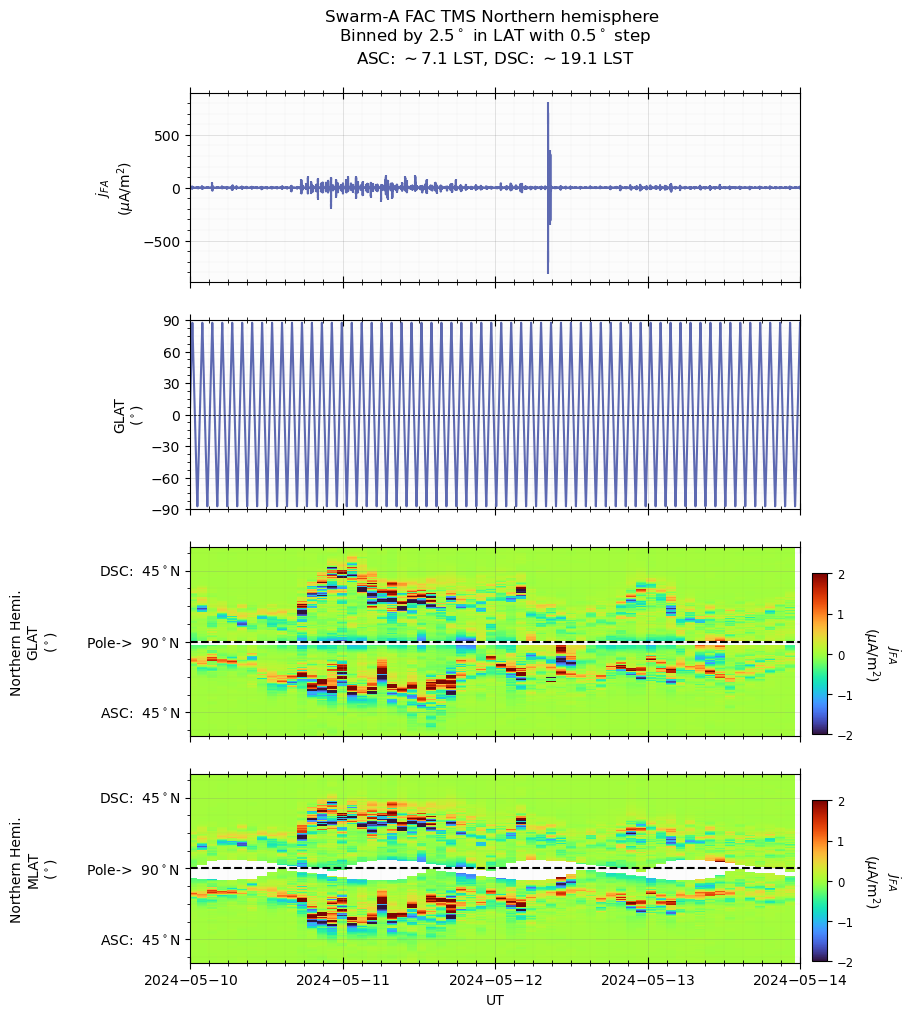
\includegraphics[width=0.7\linewidth]{files/0c22ff34ad86946d80ea8c9ee1734f18.png}

\subsection{Conjuction finder}

GeospaceLAB provides a convenient method to find conjunctions between satellite trajectories and ground station locations. The Swarm \texttt{Dataset} has the built-in method \texttt{find\_conjunctions} to find conjunctions between the Swarm satellite and a station. The following function demonstrates how to use this method to find conjunctions between the Swarm A satellite and the EISCAT Tromsø site.

This method also check the data avaibility of the Swarm data product during the conjunction time, and only return the conjunctions with data available.

\begin{verbatim}
import datetime
import matplotlib.pyplot as plt
import numpy as np
import pathlib

import geospacelab.visualization.mpl.dashboards as dashboards
\end{verbatim}

\begin{verbatim}
dt_fr = datetime.datetime(2024, 5, 10, 0, )
dt_to = datetime.datetime(2024, 5, 13, 0, 0)

site_info = {
    'glat': 69.58, 'glon': 19.23, 'alt': 0. # EISCAT Tromso site
}

db = dashboards.TSDashboard(
    dt_fr=dt_fr, dt_to=dt_to, figure_config={'figsize': (8, 10)},
    timeline_extra_labels=['GEO_LAT', 'GEO_LON', 'APEX_LAT', 'APEX_LON', 'APEX_MLT',]
    )

ds_fac = db.dock(
    datasource_contents=['esa_eo', 'swarm', 'l2daily', 'fac_tms'], 
    product_version='latest', # 'latest' (default),
    sat_id='A', add_APEX=False)

conj_list = ds_fac.get_conjunction_with_site(
        glat_site=site_info['glat'], 
        glon_site=site_info['glon'], 
        alt_site=site_info['alt'],
        # Elevation limit for conjunctions. 
        # Only conjunctions with satellite elevation above 
        # the site higher than this limit 
        # will be included in the conjunction list.
        el_lim=60.,
        # Whether to print the conjunction list.
        print_conj_list=True,
    )
\end{verbatim}

\begin{verbatim}
Create a new figure: Figure(800x1000).
\end{verbatim}

\begin{verbatim}
Load IGRF coefficients ...
\end{verbatim}

\begin{verbatim}
Searching the data product "FAC_TMS" with the version "latest" on the server...
The file [PosixPath('/data/afys -ionosphere/data/ESA/SWARM/Level2daily/FAC_TMS/0401/Sat_A/2024/SW_OPER_FACATMS_2F_20240510T000000_20240510T235959_0401.cdf')] already exists: skip downloading.
The file [PosixPath('/data/afys -ionosphere/data/ESA/SWARM/Level2daily/FAC_TMS/0401/Sat_A/2024/SW_OPER_FACATMS_2F_20240511T000000_20240511T235959_0401.cdf')] already exists: skip downloading.
The file [PosixPath('/data/afys -ionosphere/data/ESA/SWARM/Level2daily/FAC_TMS/0401/Sat_A/2024/SW_OPER_FACATMS_2F_20240512T000000_20240512T235959_0401.cdf')] already exists: skip downloading.
The file [PosixPath('/data/afys -ionosphere/data/ESA/SWARM/Level2daily/FAC_TMS/0401/Sat_A/2024/SW_OPER_FACATMS_2F_20240513T000000_20240513T235959_0401.cdf')] already exists: skip downloading.
4 conjunction(s) found:
Index  Time (Start)         EL (Start) AZ (Start) D (Start)  Time (Highest)            EL (Highest)    AZ (Highest)    D (Highest)     Time (End)           EL (End)   AZ (End)   D (End)    Duration(s)
0      2024 -05 -10 06:32:18  60.34      232.93     246.36     2024 -05 -10 06:32:51       79.66           272.73          79.71           2024 -05 -10 06:33:24  60.20      329.70     247.55     66.00     
1      2024 -05 -10 17:41:29  60.04      287.70     249.06     2024 -05 -10 17:41:55       69.08           268.60          166.19          2024 -05 -10 17:42:21  60.19      245.18     247.71     52.00     
2      2024 -05 -11 06:03:25  60.43      119.23     245.44     2024 -05 -11 06:03:53       71.16           91.13           148.55          2024 -05 -11 06:04:20  60.45      69.68      245.11     55.00     
3      2024 -05 -11 17:12:23  60.56      20.83      243.93     2024 -05 -11 17:12:56       81.87           86.84           62.33           2024 -05 -11 17:13:30  60.28      133.15     246.84     67.00
\end{verbatim}

\begin{verbatim}
<FigureBase size 800x1000 with 0 Axes>
\end{verbatim}

The following function shows the time series plots with the conjunction with the EISCAT Tromsø site. The conjunction time is indicated by the vertical dashed line in the plot.

\begin{verbatim}
def test_conjunction_with_site():
    """Test Swarm EFI/LP 1B data product
    
    """
    dt_fr = datetime.datetime(2024, 5, 10, 0, )
    dt_to = datetime.datetime(2024, 5, 13, 0, 0)

    site_info = {
        'glat': 69.58, 'glon': 19.23, 'alt': 0. # EISCAT Tromso site
    }
    
    db = dashboards.TSDashboard(
        dt_fr=dt_fr, dt_to=dt_to, figure_config={'figsize': (8, 10)},
        timeline_extra_labels=['GEO_LAT', 'GEO_LON', 'APEX_LAT', 'APEX_LON', 'APEX_MLT',]
        )

    ds_fac = db.dock(
        datasource_contents=['esa_eo', 'swarm', 'l2daily', 'fac_tms'], 
        product_version='latest', # 'latest' (default),
        sat_id='A', add_APEX=False)
    
    conj_list = ds_fac.get_conjunction_with_site(
         glat_site=site_info['glat'], 
         glon_site=site_info['glon'], 
         alt_site=site_info['alt'],
         el_lim=60.,
         print_conj_list=True,
     )
    conj_data = conj_list[1]
    dt_fr_to_show = conj_data['DATETIME_0']
    dt_to_to_show = conj_data['DATETIME_1']
    
    ds_fac.dt_fr = dt_fr_to_show
    ds_fac.dt_to = dt_to_to_show
    ds_fac.time_filter_by_range()
    ds_fac.convert_to_APEX()
    
    ds_efi_lp = db.dock(
        dt_fr=dt_fr_to_show, dt_to=dt_to_to_show,
        datasource_contents=['esa_eo', 'swarm', 'l1b', 'efi_lp'], 
        product_version='latest', # 'latest' (default),
        sat_id='A', add_APEX=True)
    
    ds_mag_lr = db.dock(
        dt_fr=dt_fr_to_show, dt_to=dt_to_to_show,
        datasource_contents=['esa_eo', 'swarm', 'l1b', 'mag_lr'], 
        from_HAPI=True,
        product_version='latest', # 'latest' (default),
        sat_id='A', add_APEX=True)
    
    panel_layouts = [
        [ds_efi_lp['n_e']],
        [ds_efi_lp['n_i']],
        [ds_efi_lp['T_e']],
        [ds_mag_lr['B_res_Model_N'], ds_mag_lr['B_res_Model_E'], ds_mag_lr['B_res_Model_C']],
        [ds_fac['j_r']],
        [ds_fac['j_FA']],
    ]

    db.set_layout(panel_layouts=panel_layouts)
    db.draw(
        dt_fr=dt_fr_to_show, dt_to=dt_to_to_show,
    )
    
    # Add a vertical line to indicate the conjunction time
    db.add_vertical_line(
        conj_data['DATETIME'], label='EISCAT TRO', color='red', linestyle=' - -', linewidth=1.5,
    )
    db.add_title(title='Swarm -{} - EISCAT Tromso conjunction'.format(ds_fac.sat_id), fontsize='medium', append_time=True)

    return db
db = test_conjunction_with_site()
db.show()
\end{verbatim}

\begin{verbatim}
Create a new figure: Figure(800x1000).
Searching the data product "FAC_TMS" with the version "latest" on the server...
The file [PosixPath('/data/afys -ionosphere/data/ESA/SWARM/Level2daily/FAC_TMS/0401/Sat_A/2024/SW_OPER_FACATMS_2F_20240510T000000_20240510T235959_0401.cdf')] already exists: skip downloading.
The file [PosixPath('/data/afys -ionosphere/data/ESA/SWARM/Level2daily/FAC_TMS/0401/Sat_A/2024/SW_OPER_FACATMS_2F_20240511T000000_20240511T235959_0401.cdf')] already exists: skip downloading.
The file [PosixPath('/data/afys -ionosphere/data/ESA/SWARM/Level2daily/FAC_TMS/0401/Sat_A/2024/SW_OPER_FACATMS_2F_20240512T000000_20240512T235959_0401.cdf')] already exists: skip downloading.
The file [PosixPath('/data/afys -ionosphere/data/ESA/SWARM/Level2daily/FAC_TMS/0401/Sat_A/2024/SW_OPER_FACATMS_2F_20240513T000000_20240513T235959_0401.cdf')] already exists: skip downloading.
4 conjunction(s) found:
Index  Time (Start)         EL (Start) AZ (Start) D (Start)  Time (Highest)            EL (Highest)    AZ (Highest)    D (Highest)     Time (End)           EL (End)   AZ (End)   D (End)    Duration(s)
0      2024 -05 -10 06:32:18  60.34      232.93     246.36     2024 -05 -10 06:32:51       79.66           272.73          79.71           2024 -05 -10 06:33:24  60.20      329.70     247.55     66.00     
1      2024 -05 -10 17:41:29  60.04      287.70     249.06     2024 -05 -10 17:41:55       69.08           268.60          166.19          2024 -05 -10 17:42:21  60.19      245.18     247.71     52.00     
2      2024 -05 -11 06:03:25  60.43      119.23     245.44     2024 -05 -11 06:03:53       71.16           91.13           148.55          2024 -05 -11 06:04:20  60.45      69.68      245.11     55.00     
3      2024 -05 -11 17:12:23  60.56      20.83      243.93     2024 -05 -11 17:12:56       81.87           86.84           62.33           2024 -05 -11 17:13:30  60.28      133.15     246.84     67.00     
Searching the data product "EFI_LP" with the version "latest" on the server...
The file [PosixPath('/data/afys -ionosphere/data/ESA/SWARM/Level1b/EFI_LP/0701/Sat_A/2024/SW_OPER_EFIA_LP_1B_20240510T000000_20240510T235959_0701_MDR_EFI_LP.cdf')] already exists: skip downloading.
/opt/anaconda3/envs/Swarm/lib/python3.12/site -packages/numpy/_core/numeric.py:476: RuntimeWarning: invalid value encountered in cast
  multiarray.copyto(res, fill_value, casting='unsafe')
INFO: Loading data from HAPI for server https://vires.services/hapi, dataset SW_OPER_MAGA_LR_1B, parameters Timestamp,Latitude,Longitude,Radius.
INFO: Data loaded from HAPI.
INFO: Loading data from HAPI for server https://vires.services/hapi, dataset SW_OPER_MAGA_LR_1B, parameters F,dF_Sun,dF_AOCS,dF_other,F_error,B_VFM,B_NEC,dB_Sun,dB_AOCS,dB_other,B_error.
INFO: Data loaded from HAPI.
INFO: Loading data from HAPI for server https://vires.services/hapi, dataset SW_OPER_MAGA_LR_1B, parameters q_NEC_CRF,Att_error,Flags_F,Flags_B,Flags_q,Flags_Platform,ASM_Freq_Dev.
INFO: Data loaded from HAPI.
INFO: Loading data from HAPI for server https://vires.services/hapi, dataset SW_OPER_MAGA_LR_1B, parameters SyncStatus,B_NEC_Model,F_Model,F_res_Model,B_NEC_res_Model.
INFO: Data loaded from HAPI.
WARNING: Variable CDF_EPOCH is not in the default variable names and does not match the patterns for automatically assigning configured variable names. It will be added without a configured variable name, and may not be included in the default panels for plotting and analysis. Please check if this variable should be included in the default variable names or if it follows the naming patterns for automatic assignment of configured variable names.
WARNING: Variable SC_GEO_R is not in the default variable names and does not match the patterns for automatically assigning configured variable names. It will be added without a configured variable name, and may not be included in the default panels for plotting and analysis. Please check if this variable should be included in the default variable names or if it follows the naming patterns for automatic assignment of configured variable names.
WARNING: Variable B_NEC_Model is not in the default variable names and does not match the patterns for automatically assigning configured variable names. It will be added without a configured variable name, and may not be included in the default panels for plotting and analysis. Please check if this variable should be included in the default variable names or if it follows the naming patterns for automatic assignment of configured variable names.
WARNING: Variable B_NEC_res_Model is not in the default variable names and does not match the patterns for automatically assigning configured variable names. It will be added without a configured variable name, and may not be included in the default panels for plotting and analysis. Please check if this variable should be included in the default variable names or if it follows the naming patterns for automatic assignment of configured variable names.
/opt/anaconda3/envs/Swarm/lib/python3.12/site -packages/numpy/_core/numeric.py:476: RuntimeWarning: invalid value encountered in cast
  multiarray.copyto(res, fill_value, casting='unsafe')
WARNING: Negative values of error detected in GeospaceLab Variable object <name: j_r, value: array([[  3.08981391],
       [  2.98925703],
       [  1.56633446],
       [ -1.13820387],
       [  1.34360429],
       [  1.20251135],
       [ -1.2249717 ],
       [  3.12994392],
       [  0.40065637],
       [ -0.16233794],
       [  5.1499497 ],
       [  0.52370211],
       [ -1.09764934],
       [  6.07112128],
       [ -0.59552206],
       [ 14.15920087],
       [  0.95167483],
       [  1.0512454 ],
       [  2.59472964],
       [  2.24155043],
       [  0.10525129],
       [ -0.12611275],
       [  2.54786862],
       [  1.12647161],
       [  2.12356771],
       [  9.03824309],
       [ -6.44872064],
       [ 20.03705361],
       [ 19.53691737],
       [ 20.52376949],
       [ -0.89872449],
       [  3.19756193],
       [  5.11868821],
       [ -4.45562301],
       [  4.36727181],
       [  9.92268407],
       [ -13.69750467],
       [ -17.54984701],
       [  0.65148948],
       [ -0.40276721],
       [ -1.6018592 ],
       [ -1.06106664],
       [  0.08647688],
       [ -0.27753619],
       [ -0.37992582],
       [  0.17879571],
       [  0.75046254],
       [ -0.13289712],
       [ -0.90712415],
       [  0.91768621],
       [  0.75739485],
       [ -1.04945885]]), unit: muA/m^2>
\end{verbatim}

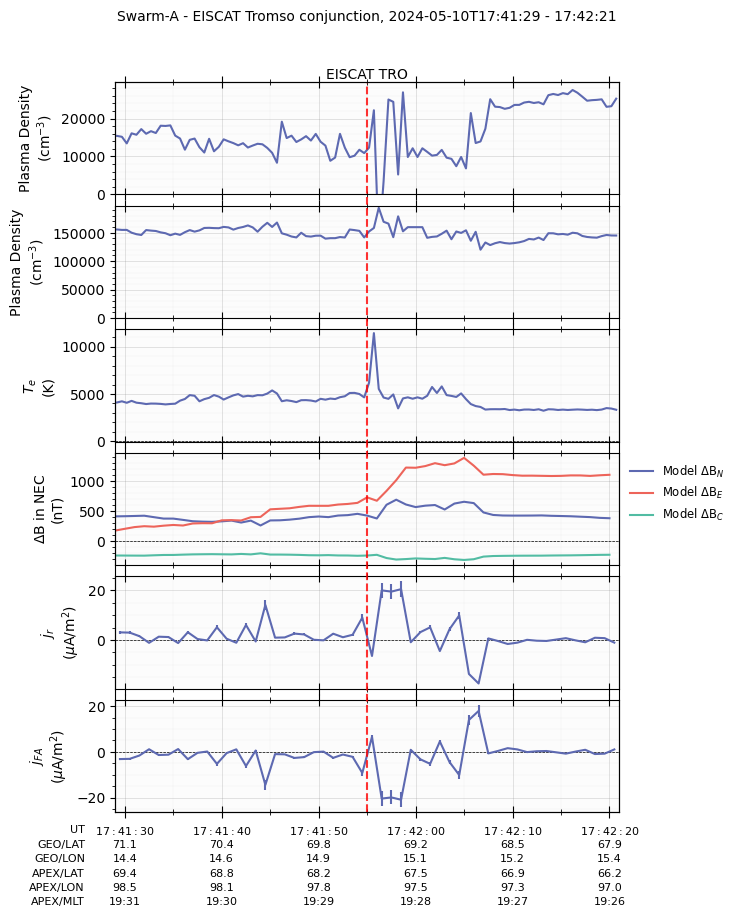
\includegraphics[width=0.7\linewidth]{files/f9eec9f1d29614cd6b8931443fa15605.png}

\subsection{Examples}

\subsubsection{Swarm MAG data products}

\begin{verbatim}
import datetime
import matplotlib.pyplot as plt
import numpy as np
import pathlib
import os

import geospacelab.visualization.mpl.dashboards as dashboards

cwd = pathlib.Path(os.path.abspath(''))
file_dir_figure = cwd / 'figures'
file_dir_figure.mkdir(parents=True, exist_ok=True)
\end{verbatim}

\paragraph{Swarm MAG LR data}

\subparagraph{Overview with a long time span}

\begin{verbatim}
def test_swarm_MAG_LR_overview():
    """Test Swarm MAG LR data product
    
    """
    dt_fr = datetime.datetime(2016, 3, 14, 12, 0)
    dt_to = datetime.datetime(2016, 3, 15, 23, 59)

    db = dashboards.TSDashboard(
        dt_fr=dt_fr, dt_to=dt_to, figure_config={'figsize': (8, 12)},
        )

    ds = db.dock(datasource_contents=['esa_eo', 'swarm', 'l1b', 'mag_lr'], sat_id='A', add_APEX=True,)

    panel_layouts = [
        [ds['F']],
        [ds['B_N'], ds['B_E'], ds['B_C']],
        [ds['B_VFM_x'], ds['B_VFM_y'], ds['B_VFM_z']],
        [ds['dB_Sun_VFM_x'], ds['dB_Sun_VFM_y'], ds['dB_Sun_VFM_z']],
        [ds['dB_AOCS_VFM_x'], ds['dB_AOCS_VFM_y'], ds['dB_AOCS_VFM_z']],
        [ds['dB_other_VFM_x'], ds['dB_other_VFM_y'], ds['dB_other_VFM_z']],
        [ds['FLAG_F_BIN_AUX']],
        [ds['FLAG_B_BIN_AUX']],
        [ds['FLAG_q_BIN_AUX']],
        [ds['FLAG_Platform_BIN_AUX']],
    ]

    db.set_layout(panel_layouts=panel_layouts)
    db.draw()
    db.add_title(title='Swarm -{} MAG LR Overview'.format(ds.sat_id), fontsize='medium', append_time=True)

    db.save_figure(
        file_dir=file_dir_figure, 
        file_name='example_MAG_LR_Swarm -{}_overview'.format(ds.sat_id), 
        dpi=100, 
        append_time=False
    )
    db.show()
test_swarm_MAG_LR_overview()
\end{verbatim}

\begin{verbatim}
Create a new figure: Figure(800x1200).
\end{verbatim}

\begin{verbatim}
Load IGRF coefficients ...
\end{verbatim}

\begin{verbatim}
Searching the data product "MAG_LR" with the version "latest" on the server...
The file [PosixPath('/data/afys -ionosphere/data/ESA/SWARM/Level1b/MAG_LR/0701/Sat_A/2016/SW_OPER_MAGA_LR_1B_20160314T000000_20160314T235959_0701_ASM_VFM_IC.cdf'), PosixPath('/data/afys -ionosphere/data/ESA/SWARM/Level1b/MAG_LR/0701/Sat_A/2016/SW_OPER_MAGA_LR_1B_20160314T000000_20160314T235959_0701_MDR_MAG_LR.cdf')] already exists: skip downloading.
The file [PosixPath('/data/afys -ionosphere/data/ESA/SWARM/Level1b/MAG_LR/0701/Sat_A/2016/SW_OPER_MAGA_LR_1B_20160315T000000_20160315T235959_0701_MDR_MAG_LR.cdf'), PosixPath('/data/afys -ionosphere/data/ESA/SWARM/Level1b/MAG_LR/0701/Sat_A/2016/SW_OPER_MAGA_LR_1B_20160315T000000_20160315T235959_0701_ASM_VFM_IC.cdf')] already exists: skip downloading.
WARNING: Multiple files found for the pattern *20160314T000000*20160314T235959*0701*.cdf in the directory /data/afys -ionosphere/data/ESA/SWARM/Level1b/MAG_LR/0701/Sat_A/2016!
WARNING: Multiple files found for the pattern *20160315T000000*20160315T235959*0701*.cdf in the directory /data/afys -ionosphere/data/ESA/SWARM/Level1b/MAG_LR/0701/Sat_A/2016!
/opt/anaconda3/envs/Swarm/lib/python3.12/site -packages/numpy/_core/numeric.py:476: RuntimeWarning: invalid value encountered in cast
  multiarray.copyto(res, fill_value, casting='unsafe')
\end{verbatim}

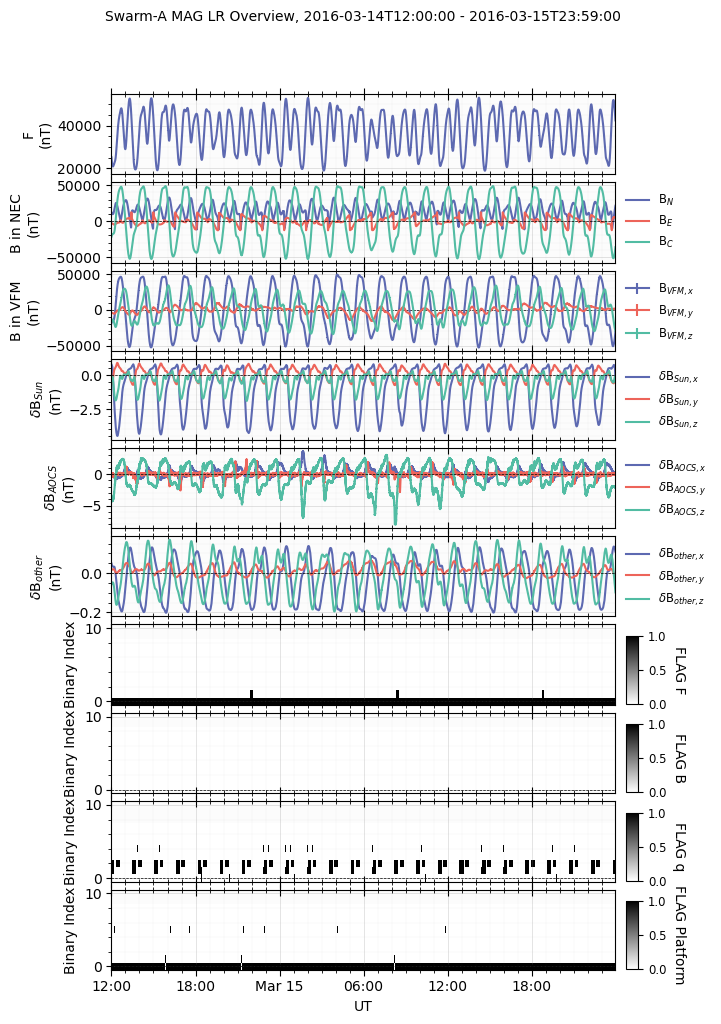
\includegraphics[width=0.7\linewidth]{files/12be9de16ba06b3da42497f3e3204f8d.png}

\subparagraph{Zoomed-in view with a short time span}

\begin{verbatim}
def test_swarm_MAG_LR_zoom():
    """Test Swarm MAG LR data product
    
    """
    dt_fr = datetime.datetime(2016, 3, 15, 18, 18)
    dt_to = datetime.datetime(2016, 3, 15, 18, 23)

    db = dashboards.TSDashboard(
        dt_fr=dt_fr, dt_to=dt_to, figure_config={'figsize': (8, 12)},
        timeline_extra_labels=['GEO_LAT', 'GEO_LON', 'APEX_LAT', 'APEX_LON', 'APEX_MLT',]  # Not applicable for very scattered data points like AEJ_PBS peaks
        )

    ds = db.dock(datasource_contents=['esa_eo', 'swarm', 'l1b', 'mag_lr'], sat_id='A', add_APEX=True,)

    panel_layouts = [
        [ds['F']],
        [ds['B_N'], ds['B_E'], ds['B_C']],
        [ds['B_VFM_x'], ds['B_VFM_y'], ds['B_VFM_z']],
        [ds['dB_Sun_VFM_x'], ds['dB_Sun_VFM_y'], ds['dB_Sun_VFM_z']],
        [ds['dB_AOCS_VFM_x'], ds['dB_AOCS_VFM_y'], ds['dB_AOCS_VFM_z']],
        [ds['dB_other_VFM_x'], ds['dB_other_VFM_y'], ds['dB_other_VFM_z']],
        [ds['FLAG_F_BIN_AUX']],
        [ds['FLAG_B_BIN_AUX']],
        [ds['FLAG_q_BIN_AUX']],
        [ds['FLAG_Platform_BIN_AUX']],
    ]

    db.set_layout(panel_layouts=panel_layouts)
    db.draw()
    db.add_title(title='Swarm -{} MAG LR Zoom'.format(ds.sat_id), fontsize='medium', append_time=True)
    
    db.save_figure(
        file_dir=file_dir_figure, 
        file_name='example_MAG_LR_Swarm -{}_zoom'.format(ds.sat_id), 
        dpi=100, 
        append_time=False
    )
    db.show()
test_swarm_MAG_LR_zoom()
\end{verbatim}

\begin{verbatim}
Create a new figure: Figure(800x1200).
Searching the data product "MAG_LR" with the version "latest" on the server...
The file [PosixPath('/data/afys -ionosphere/data/ESA/SWARM/Level1b/MAG_LR/0701/Sat_A/2016/SW_OPER_MAGA_LR_1B_20160315T000000_20160315T235959_0701_MDR_MAG_LR.cdf'), PosixPath('/data/afys -ionosphere/data/ESA/SWARM/Level1b/MAG_LR/0701/Sat_A/2016/SW_OPER_MAGA_LR_1B_20160315T000000_20160315T235959_0701_ASM_VFM_IC.cdf')] already exists: skip downloading.
WARNING: Multiple files found for the pattern *20160315T000000*20160315T235959*0701*.cdf in the directory /data/afys -ionosphere/data/ESA/SWARM/Level1b/MAG_LR/0701/Sat_A/2016!
\end{verbatim}

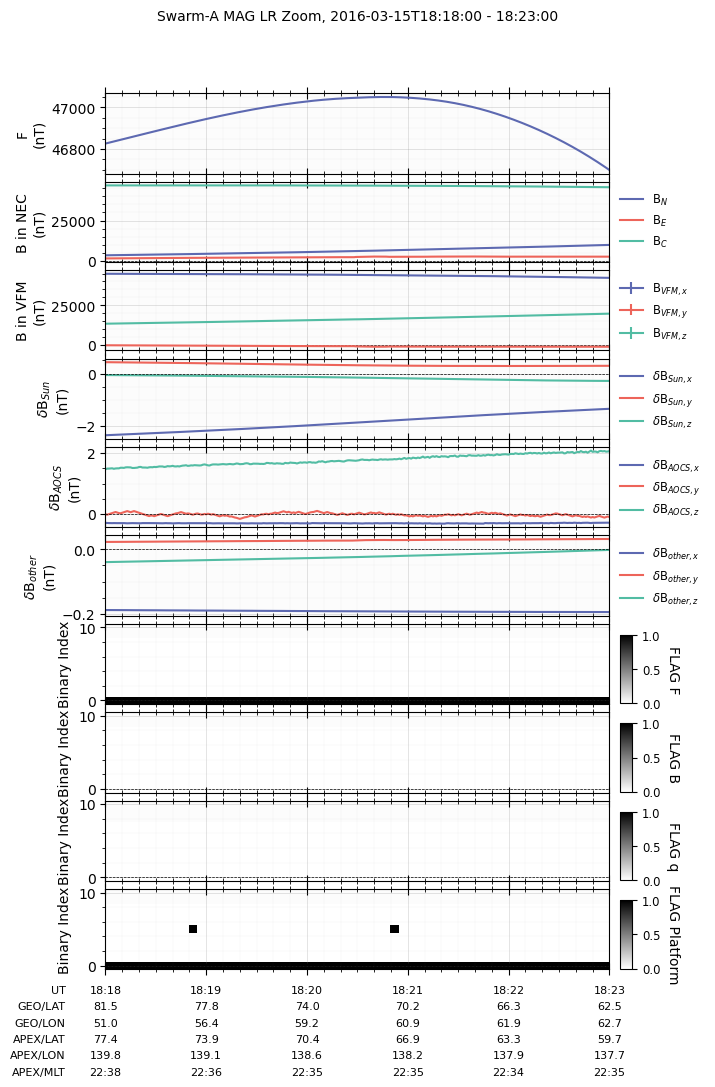
\includegraphics[width=0.7\linewidth]{files/fbdd1a64bfbcfd166df6f2202707e003.png}

\paragraph{Swarm MAG HR data}

\begin{verbatim}
def test_swarm_MAG_HR_zoom():
    """Test Swarm MAG HR data product
    
    """
    dt_fr = datetime.datetime(2016, 3, 15, 18, 18)
    dt_to = datetime.datetime(2016, 3, 15, 18, 23)

    db = dashboards.TSDashboard(
        dt_fr=dt_fr, dt_to=dt_to, figure_config={'figsize': (8, 12)},
        timeline_extra_labels=['GEO_LAT', 'GEO_LON', 'APEX_LAT', 'APEX_LON', 'APEX_MLT',]  # Not applicable for very scattered data points like AEJ_PBS peaks
        )

    ds = db.dock(datasource_contents=['esa_eo', 'swarm', 'l1b', 'mag_hr'], sat_id='A', add_APEX=True,)

    panel_layouts = [
        [ds['B_N'], ds['B_E'], ds['B_C']],
        [ds['B_VFM_x'], ds['B_VFM_y'], ds['B_VFM_z']],
        [ds['dB_Sun_VFM_x'], ds['dB_Sun_VFM_y'], ds['dB_Sun_VFM_z']],
        [ds['dB_AOCS_VFM_x'], ds['dB_AOCS_VFM_y'], ds['dB_AOCS_VFM_z']],
        [ds['dB_other_VFM_x'], ds['dB_other_VFM_y'], ds['dB_other_VFM_z']],
        [ds['FLAG_B_BIN_AUX']],
        [ds['FLAG_q_BIN_AUX']],
        [ds['FLAG_Platform_BIN_AUX']],
    ]

    db.set_layout(panel_layouts=panel_layouts)
    db.draw()
    db.add_title(title='Swarm -{} MAG HR Zoom'.format(ds.sat_id), fontsize='medium', append_time=True)
    
    db.save_figure(
        file_dir=file_dir_figure, 
        file_name='example_MAG_HR_Swarm -{}_zoom'.format(ds.sat_id), 
        dpi=100, 
        append_time=False
    )
    db.show()
test_swarm_MAG_HR_zoom()
\end{verbatim}

\begin{verbatim}
Create a new figure: Figure(800x1200).
Searching the data product "MAG_HR" with the version "latest" on the server...
INFO: Indexing the files for the product MAG_HR of the satellite A ...
The file [PosixPath('/data/afys -ionosphere/data/ESA/SWARM/Level1b/MAG_HR/0701/Sat_A/2016/SW_OPER_MAGA_HR_1B_20160315T000000_20160315T235959_0701_MDR_MAG_HR.cdf'), PosixPath('/data/afys -ionosphere/data/ESA/SWARM/Level1b/MAG_HR/0701/Sat_A/2016/SW_OPER_MAGA_HR_1B_20160315T000000_20160315T235959_0701_ASM_VFM_IC.cdf')] already exists: skip downloading.
WARNING: Multiple files found for the pattern *20160315T000000*20160315T235959*0701*.cdf in the directory /data/afys -ionosphere/data/ESA/SWARM/Level1b/MAG_HR/0701/Sat_A/2016!
\end{verbatim}

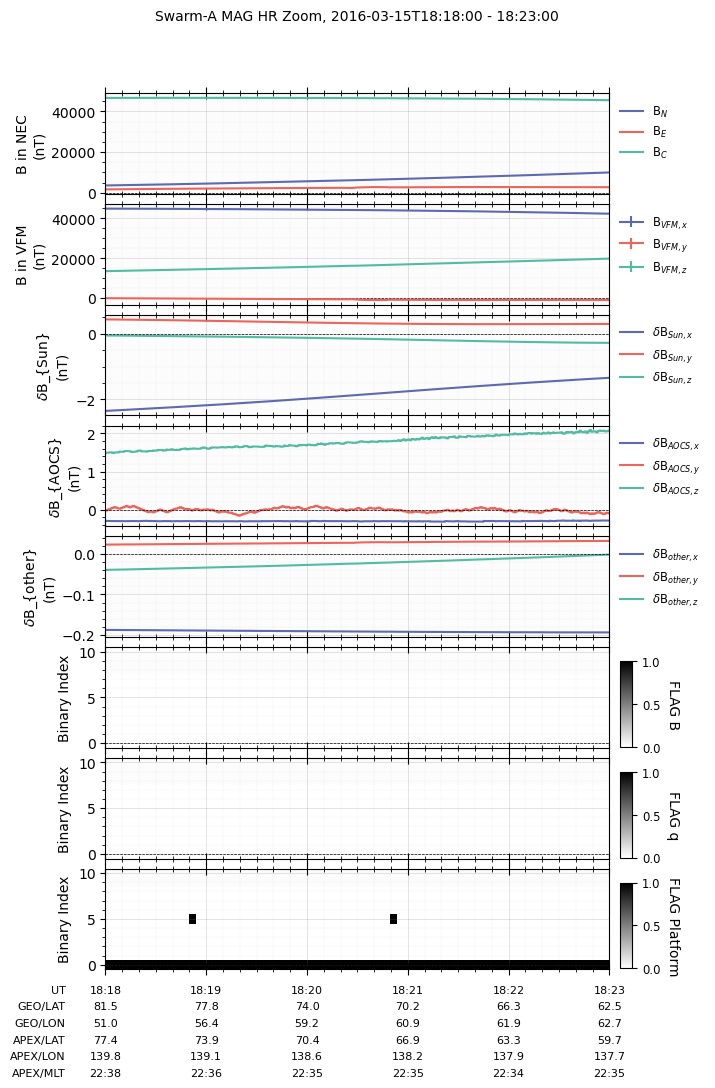
\includegraphics[width=0.7\linewidth]{files/bf8bac4495659d64665ba9d1dd6c0234.png}

\paragraph{Swarm MAG LR data from Swarm VirES service}

\subparagraph{With CHAOS modeled B-field}

\begin{verbatim}
def test_swarm_MAG_LR_from_VirES_OPER():
    """Test loading Swarm MAG LR data product from VirES

    """
    dt_fr = datetime.datetime(2016, 3, 15, 18, 18)
    dt_to = datetime.datetime(2016, 3, 15, 18, 23)

    # Default kwargs for VirES data loading, which can be overridden when calling the dock method to load data from VirES. The measurements, models, and residuals to load can be specified in the kwargs_products dictionary. The default settings are for loading all available measurements and models, and no residuals. The available measurements and models depend on the specific collection and product being loaded, and can be checked in the VirES API documentation or by inspecting the variables in the loaded dataset.
    kwargs_products_default = {
            "measurements": [
                'B_VFM', 'B_NEC', 'dB_Sun', 'dB_AOCS', 'dB_other', 'B_error',
                'q_NEC_CRF', 'Att_error',
                'Flags_B', 'Flags_q', 'Flags_Platform', 'Flags_F',
                'ASM_Freq_Dev', 'F', 'F_error', 'dF_Sun', 'dF_AOCS', 'dF_other',
            ],
            "models": [
                'CHAOS -Core',
            ],
            "residuals": False,
        }
    
    
    db = dashboards.TSDashboard(
        dt_fr=dt_fr, dt_to=dt_to, figure_config={'figsize': (8, 12)},
        timeline_extra_labels=['GEO_LAT', 'GEO_LON', 'APEX_LAT', 'APEX_LON', 'APEX_MLT',]  # Not applicable for very scattered data points like AEJ_PBS peaks
        )

    ds = db.dock(
        datasource_contents=['esa_eo', 'swarm', 'l1b', 'mag_lr'], 
        from_VirES=True, from_FAST=False,
        sat_id='A', add_APEX=True,
        kwargs_VirES={"kwargs_products": kwargs_products_default},
    )

    panel_layouts = [
        [ds['F']],
        [ds['B_N'], ds['B_E'], ds['B_C']],
        [ds['B_VFM_x'], ds['B_VFM_y'], ds['B_VFM_z']],
        [ds['dB_Sun_VFM_x'], ds['dB_Sun_VFM_y'], ds['dB_Sun_VFM_z']],
        [ds['dB_AOCS_VFM_x'], ds['dB_AOCS_VFM_y'], ds['dB_AOCS_VFM_z']],
        [ds['dB_other_VFM_x'], ds['dB_other_VFM_y'], ds['dB_other_VFM_z']],
        [ds['FLAG_F_BIN_AUX']],
        [ds['FLAG_B_BIN_AUX']],
        [ds['FLAG_q_BIN_AUX']],
        [ds['FLAG_Platform_BIN_AUX']],
    ]

    db.set_layout(panel_layouts=panel_layouts)
    db.draw()
    db.add_title(title='Swarm -{} MAG LR Zoom from VirES OPER'.format(ds.sat_id), fontsize='medium', append_time=True)
    
    db.save_figure(
        file_dir=file_dir_figure, 
        file_name='example_MAG_LR_Swarm -{}_zoom_VirES_OPER'.format(ds.sat_id), 
        dpi=100, 
        append_time=False
    )
    db.show()
test_swarm_MAG_LR_from_VirES_OPER()
\end{verbatim}

\begin{verbatim}
Create a new figure: Figure(800x1200).
INFO: Loading data from VirES for collection SW_OPER_MAGA_LR_1B with products {'measurements': ['B_VFM', 'B_NEC', 'dB_Sun', 'dB_AOCS', 'dB_other', 'B_error', 'q_NEC_CRF', 'Att_error', 'Flags_B', 'Flags_q', 'Flags_Platform', 'Flags_F', 'ASM_Freq_Dev', 'F', 'F_error', 'dF_Sun', 'dF_AOCS', 'dF_other'], 'models': ['CHAOS -Core'], 'residuals': False}.
Processing:  100%|██████████|  [ Elapsed: 00:00, Remaining: 00:00 ] [1/1] 
Downloading: 100%|██████████|  [ Elapsed: 00:00, Remaining: 00:00 ] (0.219MB)
INFO: Data loaded from VirES.
WARNING: Variable name Spacecraft not found in the variable name dictionary, and no unique match found. Skipping this variable.
WARNING: Variable SC_GEO_R is not in the default variable names and does not match the patterns for automatically assigning configured variable names. It will be added without a configured variable name, and may not be included in the default panels for plotting and analysis. Please check if this variable should be included in the default variable names or if it follows the naming patterns for automatic assignment of configured variable names.
WARNING: Variable B_NEC_CHAOS -Core is not in the default variable names and does not match the patterns for automatically assigning configured variable names. It will be added without a configured variable name, and may not be included in the default panels for plotting and analysis. Please check if this variable should be included in the default variable names or if it follows the naming patterns for automatic assignment of configured variable names.
/opt/anaconda3/envs/Swarm/lib/python3.12/site -packages/numpy/_core/numeric.py:476: RuntimeWarning: invalid value encountered in cast
  multiarray.copyto(res, fill_value, casting='unsafe')
\end{verbatim}

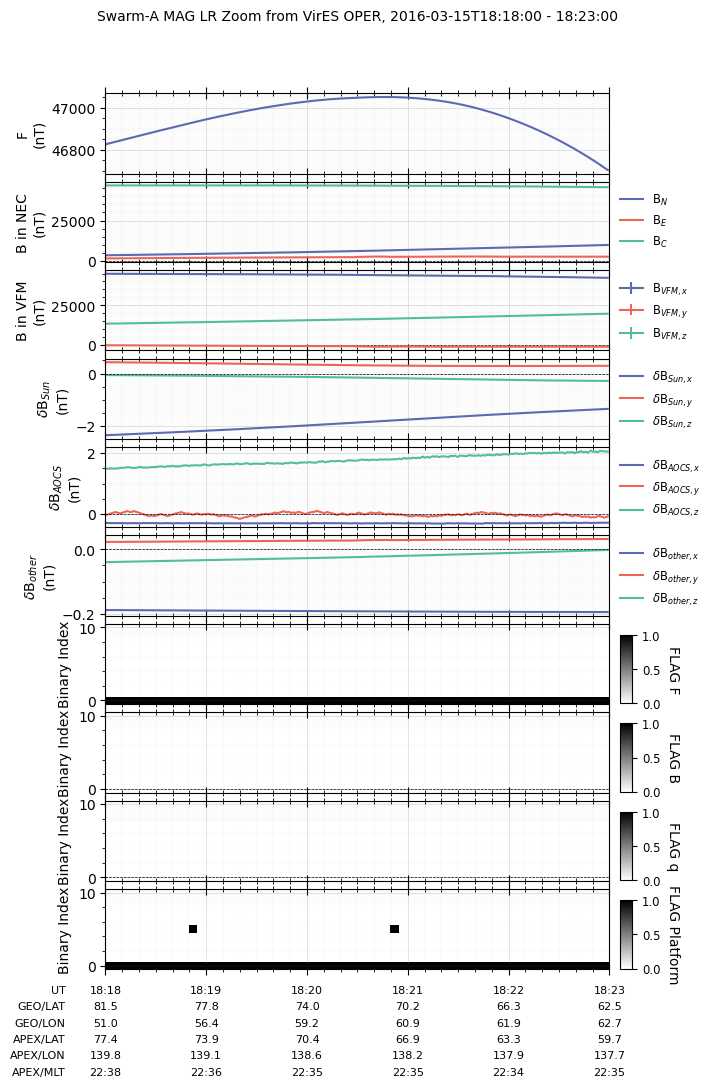
\includegraphics[width=0.7\linewidth]{files/455693ca58666f74048290f5d9079a75.png}

\subparagraph{With CHAOS modeled B-field disturbances}

\begin{verbatim}
def test_swarm_MAG_LR_from_VirES_OPER_Residuals():
    """Test loading Swarm MAG LR data product from VirES

    """
    dt_fr = datetime.datetime(2016, 3, 15, 18, 18)
    dt_to = datetime.datetime(2016, 3, 15, 18, 23)

    # Default kwargs for VirES data loading, which can be overridden when calling the dock method to load data from VirES. The measurements, models, and residuals to load can be specified in the kwargs_products dictionary. The default settings are for loading all available measurements and models, and no residuals. The available measurements and models depend on the specific collection and product being loaded, and can be checked in the VirES API documentation or by inspecting the variables in the loaded dataset.
    kwargs_products_default = {
            "measurements": [
                'B_VFM', 'B_NEC', 'dB_Sun', 'dB_AOCS', 'dB_other', 'B_error',
                'q_NEC_CRF', 'Att_error',
                'Flags_B', 'Flags_q', 'Flags_Platform', 'Flags_F',
                'ASM_Freq_Dev', 'F', 'F_error', 'dF_Sun', 'dF_AOCS', 'dF_other',
            ],
            "models": [
                'CHAOS -Core',
            ],
            "residuals": True,
        }
    
    
    db = dashboards.TSDashboard(
        dt_fr=dt_fr, dt_to=dt_to, figure_config={'figsize': (8, 12)},
        timeline_extra_labels=['GEO_LAT', 'GEO_LON', 'APEX_LAT', 'APEX_LON', 'APEX_MLT',]  # Not applicable for very scattered data points like AEJ_PBS peaks
        )

    ds = db.dock(
        datasource_contents=['esa_eo', 'swarm', 'l1b', 'mag_lr'], 
        from_VirES=True, from_FAST=False,
        sat_id='A', add_APEX=True,
        kwargs_VirES={"kwargs_products": kwargs_products_default},
    )

    panel_layouts = [
        [ds['F_res_CHAOS -Core']],
        [ds['B_res_CHAOS -Core_N'], ds['B_res_CHAOS -Core_E'], ds['B_res_CHAOS -Core_C']],
        [ds['B_VFM_x'], ds['B_VFM_y'], ds['B_VFM_z']],
        [ds['dB_Sun_VFM_x'], ds['dB_Sun_VFM_y'], ds['dB_Sun_VFM_z']],
        [ds['dB_AOCS_VFM_x'], ds['dB_AOCS_VFM_y'], ds['dB_AOCS_VFM_z']],
        [ds['dB_other_VFM_x'], ds['dB_other_VFM_y'], ds['dB_other_VFM_z']],
        [ds['FLAG_F_BIN_AUX']],
        [ds['FLAG_B_BIN_AUX']],
        [ds['FLAG_q_BIN_AUX']],
        [ds['FLAG_Platform_BIN_AUX']],
    ]

    db.set_layout(panel_layouts=panel_layouts)
    db.draw()
    db.add_title(title='Swarm -{} MAG LR Zoom from VirES OPER'.format(ds.sat_id), fontsize='medium', append_time=True)
    
    db.save_figure(
        file_dir=file_dir_figure, 
        file_name='example_MAG_LR_Swarm -{}_zoom_VirES_OPER_Residuals'.format(ds.sat_id), 
        dpi=100, 
        append_time=False
    )
    db.show()
test_swarm_MAG_LR_from_VirES_OPER_Residuals()
\end{verbatim}

\begin{verbatim}
Create a new figure: Figure(800x1200).
INFO: Loading data from VirES for collection SW_OPER_MAGA_LR_1B with products {'measurements': ['B_VFM', 'B_NEC', 'dB_Sun', 'dB_AOCS', 'dB_other', 'B_error', 'q_NEC_CRF', 'Att_error', 'Flags_B', 'Flags_q', 'Flags_Platform', 'Flags_F', 'ASM_Freq_Dev', 'F', 'F_error', 'dF_Sun', 'dF_AOCS', 'dF_other'], 'models': ['CHAOS -Core'], 'residuals': True}.
Processing:  100%|██████████|  [ Elapsed: 00:01, Remaining: 00:00 ] [1/1] 
Downloading: 100%|██████████|  [ Elapsed: 00:00, Remaining: 00:00 ] (0.202MB)
INFO: Data loaded from VirES.
WARNING: Variable name Spacecraft not found in the variable name dictionary, and no unique match found. Skipping this variable.
WARNING: Variable SC_GEO_R is not in the default variable names and does not match the patterns for automatically assigning configured variable names. It will be added without a configured variable name, and may not be included in the default panels for plotting and analysis. Please check if this variable should be included in the default variable names or if it follows the naming patterns for automatic assignment of configured variable names.
WARNING: Variable B_NEC_res_CHAOS -Core is not in the default variable names and does not match the patterns for automatically assigning configured variable names. It will be added without a configured variable name, and may not be included in the default panels for plotting and analysis. Please check if this variable should be included in the default variable names or if it follows the naming patterns for automatic assignment of configured variable names.
/opt/anaconda3/envs/Swarm/lib/python3.12/site -packages/numpy/_core/numeric.py:476: RuntimeWarning: invalid value encountered in cast
  multiarray.copyto(res, fill_value, casting='unsafe')
\end{verbatim}

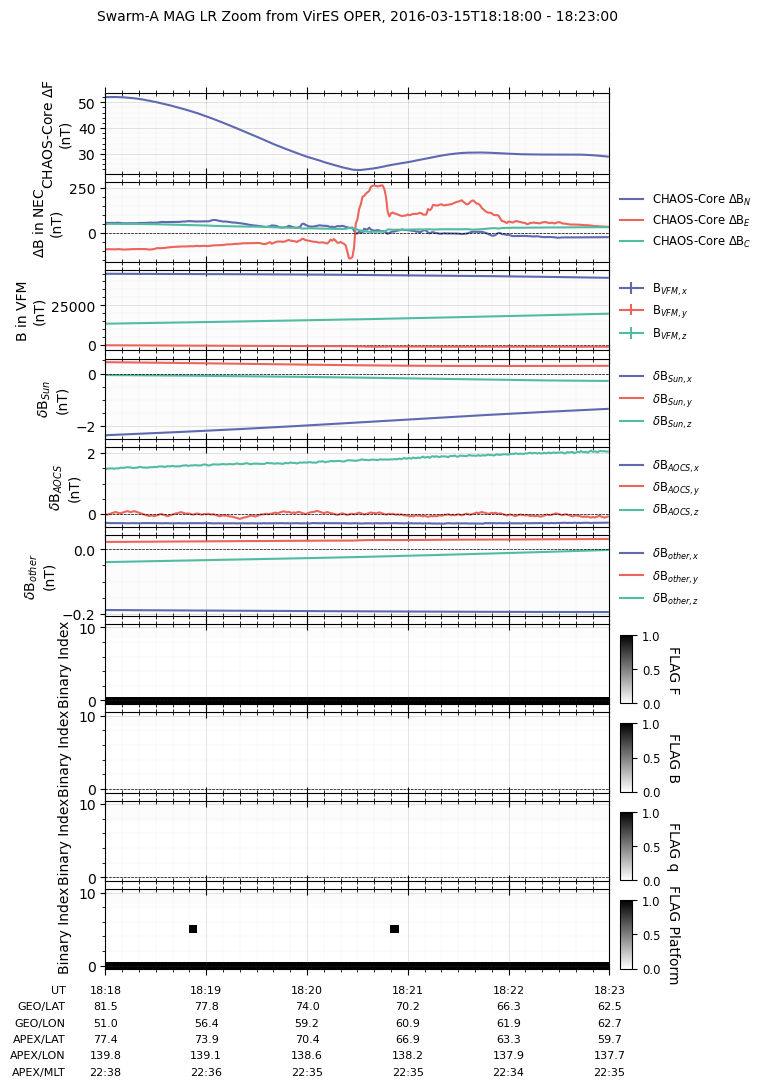
\includegraphics[width=0.7\linewidth]{files/10ae0363ce42a0130cd0276a59108004.png}

\subparagraph{Swarm MAG LR FAST data from Swarm VirES service}

\begin{verbatim}
def test_swarm_MAG_LR_from_VirES_FAST():
    """Test loading Swarm MAG LR data product from VirES

    """
    dt_fr = datetime.datetime(2026, 3, 21, 18, 00)
    dt_to = datetime.datetime(2026, 3, 21, 18, 16)

    # Default kwargs for VirES data loading, which can be overridden when calling the dock method to load data from VirES. The measurements, models, and residuals to load can be specified in the kwargs_products dictionary. The default settings are for loading all available measurements and models, and no residuals. The available measurements and models depend on the specific collection and product being loaded, and can be checked in the VirES API documentation or by inspecting the variables in the loaded dataset.
    kwargs_products_default = {
            "measurements": [
                'B_VFM', 'B_NEC', 'dB_Sun', 'dB_AOCS', 'dB_other', 'B_error',
                'q_NEC_CRF', 'Att_error',
                'Flags_B', 'Flags_q', 'Flags_Platform', 'Flags_F',
                'ASM_Freq_Dev', 'F', 'F_error', 'dF_Sun', 'dF_AOCS', 'dF_other',
            ],
            "models": [
                'CHAOS -Core',
            ],
            "residuals": False,
        }
    
    
    db = dashboards.TSDashboard(
        dt_fr=dt_fr, dt_to=dt_to, figure_config={'figsize': (8, 12)},
        timeline_extra_labels=['GEO_LAT', 'GEO_LON', 'APEX_LAT', 'APEX_LON', 'APEX_MLT',]  # Not applicable for very scattered data points like AEJ_PBS peaks
        )

    ds = db.dock(
        datasource_contents=['esa_eo', 'swarm', 'l1b', 'mag_lr'], 
        from_VirES=True, from_FAST=True,
        sat_id='A', add_APEX=True,
        kwargs_VirES={"kwargs_products": kwargs_products_default},
    )

    panel_layouts = [
        [ds['F']],
        [ds['B_N'], ds['B_E'], ds['B_C']],
        [ds['B_VFM_x'], ds['B_VFM_y'], ds['B_VFM_z']],
        [ds['dB_Sun_VFM_x'], ds['dB_Sun_VFM_y'], ds['dB_Sun_VFM_z']],
        [ds['dB_AOCS_VFM_x'], ds['dB_AOCS_VFM_y'], ds['dB_AOCS_VFM_z']],
        [ds['dB_other_VFM_x'], ds['dB_other_VFM_y'], ds['dB_other_VFM_z']],
        [ds['FLAG_F_BIN_AUX']],
        [ds['FLAG_B_BIN_AUX']],
        [ds['FLAG_q_BIN_AUX']],
        [ds['FLAG_Platform_BIN_AUX']],
    ]

    db.set_layout(panel_layouts=panel_layouts)
    db.draw()
    db.add_title(title='Swarm -{} MAG LR Zoom from VirES FAST'.format(ds.sat_id), fontsize='medium', append_time=True)
    
    db.save_figure(
        file_dir=file_dir_figure, 
        file_name='example_MAG_LR_Swarm -{}_zoom_VirES_FAST'.format(ds.sat_id), 
        dpi=100, 
        append_time=False
    )
    db.show()
test_swarm_MAG_LR_from_VirES_FAST()
\end{verbatim}

\begin{verbatim}
Create a new figure: Figure(800x1200).
INFO: Loading data from VirES for collection SW_FAST_MAGA_LR_1B with products {'measurements': ['B_VFM', 'B_NEC', 'dB_Sun', 'dB_AOCS', 'dB_other', 'B_error', 'q_NEC_CRF', 'Att_error', 'Flags_B', 'Flags_q', 'Flags_Platform', 'Flags_F', 'ASM_Freq_Dev', 'F', 'F_error', 'dF_Sun', 'dF_AOCS', 'dF_other'], 'models': ['CHAOS -Core'], 'residuals': False}.
Processing:  100%|██████████|  [ Elapsed: 00:01, Remaining: 00:00 ] [1/1] 
Downloading: 100%|██████████|  [ Elapsed: 00:00, Remaining: 00:00 ] (0.344MB)
INFO: Data loaded from VirES.
WARNING: Variable name Spacecraft not found in the variable name dictionary, and no unique match found. Skipping this variable.
WARNING: Variable SC_GEO_R is not in the default variable names and does not match the patterns for automatically assigning configured variable names. It will be added without a configured variable name, and may not be included in the default panels for plotting and analysis. Please check if this variable should be included in the default variable names or if it follows the naming patterns for automatic assignment of configured variable names.
WARNING: Variable B_NEC_CHAOS -Core is not in the default variable names and does not match the patterns for automatically assigning configured variable names. It will be added without a configured variable name, and may not be included in the default panels for plotting and analysis. Please check if this variable should be included in the default variable names or if it follows the naming patterns for automatic assignment of configured variable names.
/opt/anaconda3/envs/Swarm/lib/python3.12/site -packages/numpy/_core/numeric.py:476: RuntimeWarning: invalid value encountered in cast
  multiarray.copyto(res, fill_value, casting='unsafe')
\end{verbatim}

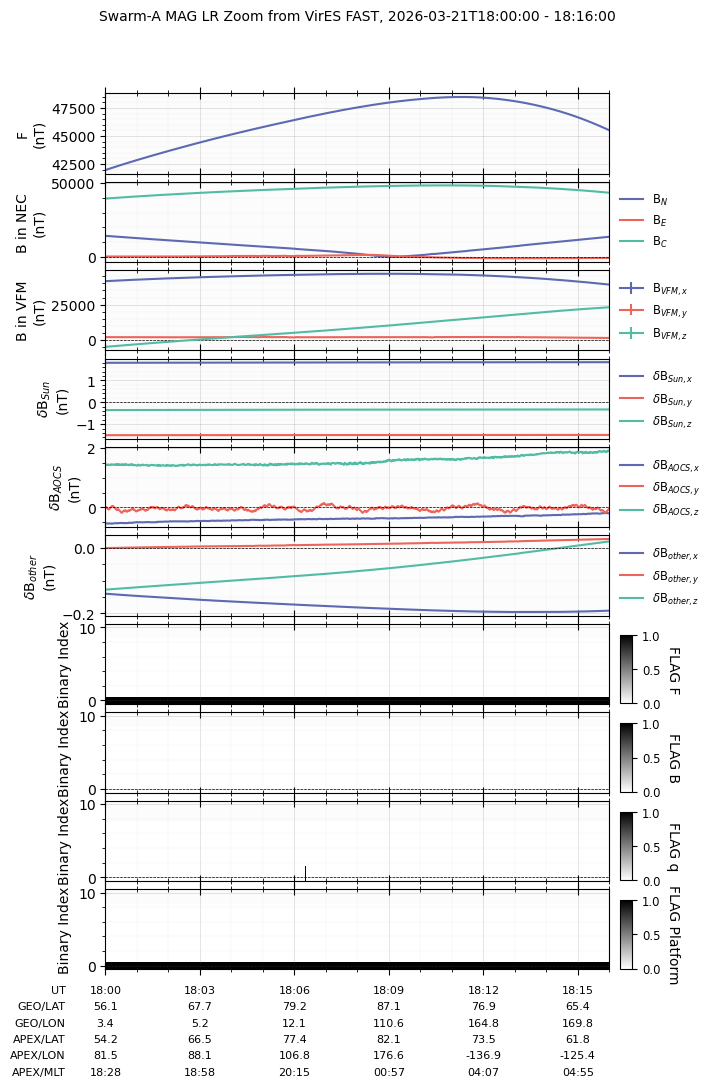
\includegraphics[width=0.7\linewidth]{files/4939f5b20234c844cd83e5b2d544119a.png}

\paragraph{Swarm MAG LR from VirES HAPI service}

\subparagraph{With CHAOS modeled B-field disturbances}

\begin{verbatim}
def test_swarm_MAG_LR_from_HAPI_OPER():
    """Test loading Swarm MAG LR data product from HAPI

    """
    dt_fr = datetime.datetime(2016, 3, 15, 18, 18)
    dt_to = datetime.datetime(2016, 3, 15, 18, 23)    
    
    db = dashboards.TSDashboard(
        dt_fr=dt_fr, dt_to=dt_to, figure_config={'figsize': (8, 12)},
        timeline_extra_labels=['GEO_LAT', 'GEO_LON', 'APEX_LAT', 'APEX_LON', 'APEX_MLT',]  # Not applicable for very scattered data points like AEJ_PBS peaks
        )

    ds = db.dock(
        datasource_contents=['esa_eo', 'swarm', 'l1b', 'mag_lr'], 
        from_HAPI=True, from_FAST=False,
        sat_id='A', add_APEX=True,
    )

    panel_layouts = [
        [ds['F']],
        [ds['F_res_Model']],
        [ds['B_N'], ds['B_E'], ds['B_C']],
        [ds['B_res_Model_N'], ds['B_res_Model_E'], ds['B_res_Model_C']],
        [ds['B_VFM_x'], ds['B_VFM_y'], ds['B_VFM_z']],
        [ds['dB_Sun_VFM_x'], ds['dB_Sun_VFM_y'], ds['dB_Sun_VFM_z']],
        [ds['dB_AOCS_VFM_x'], ds['dB_AOCS_VFM_y'], ds['dB_AOCS_VFM_z']],
        [ds['dB_other_VFM_x'], ds['dB_other_VFM_y'], ds['dB_other_VFM_z']],
        [ds['FLAG_F_BIN_AUX']],
        [ds['FLAG_B_BIN_AUX']],
        [ds['FLAG_q_BIN_AUX']],
        [ds['FLAG_Platform_BIN_AUX']],
    ]

    db.set_layout(panel_layouts=panel_layouts)
    db.draw()
    db.add_title(title='Swarm -{} MAG LR Zoom from HAPI OPER'.format(ds.sat_id), fontsize='medium', append_time=True)
    
    db.save_figure(
        file_dir=file_dir_figure, 
        file_name='example_MAG_LR_Swarm -{}_zoom_HAPI_OPER'.format(ds.sat_id), 
        dpi=100, 
        append_time=False
    )
    db.show()
test_swarm_MAG_LR_from_HAPI_OPER()
\end{verbatim}

\begin{verbatim}
Create a new figure: Figure(800x1200).
INFO: Loading data from HAPI for server https://vires.services/hapi, dataset SW_OPER_MAGA_LR_1B, parameters Timestamp,Latitude,Longitude,Radius.
INFO: Data loaded from HAPI.
INFO: Loading data from HAPI for server https://vires.services/hapi, dataset SW_OPER_MAGA_LR_1B, parameters F,dF_Sun,dF_AOCS,dF_other,F_error,B_VFM,B_NEC,dB_Sun,dB_AOCS,dB_other,B_error.
INFO: Data loaded from HAPI.
INFO: Loading data from HAPI for server https://vires.services/hapi, dataset SW_OPER_MAGA_LR_1B, parameters q_NEC_CRF,Att_error,Flags_F,Flags_B,Flags_q,Flags_Platform,ASM_Freq_Dev.
INFO: Data loaded from HAPI.
INFO: Loading data from HAPI for server https://vires.services/hapi, dataset SW_OPER_MAGA_LR_1B, parameters SyncStatus,B_NEC_Model,F_Model,F_res_Model,B_NEC_res_Model.
INFO: Data loaded from HAPI.
WARNING: Variable CDF_EPOCH is not in the default variable names and does not match the patterns for automatically assigning configured variable names. It will be added without a configured variable name, and may not be included in the default panels for plotting and analysis. Please check if this variable should be included in the default variable names or if it follows the naming patterns for automatic assignment of configured variable names.
WARNING: Variable SC_GEO_R is not in the default variable names and does not match the patterns for automatically assigning configured variable names. It will be added without a configured variable name, and may not be included in the default panels for plotting and analysis. Please check if this variable should be included in the default variable names or if it follows the naming patterns for automatic assignment of configured variable names.
WARNING: Variable B_NEC_Model is not in the default variable names and does not match the patterns for automatically assigning configured variable names. It will be added without a configured variable name, and may not be included in the default panels for plotting and analysis. Please check if this variable should be included in the default variable names or if it follows the naming patterns for automatic assignment of configured variable names.
WARNING: Variable B_NEC_res_Model is not in the default variable names and does not match the patterns for automatically assigning configured variable names. It will be added without a configured variable name, and may not be included in the default panels for plotting and analysis. Please check if this variable should be included in the default variable names or if it follows the naming patterns for automatic assignment of configured variable names.
/opt/anaconda3/envs/Swarm/lib/python3.12/site -packages/numpy/_core/numeric.py:476: RuntimeWarning: invalid value encountered in cast
  multiarray.copyto(res, fill_value, casting='unsafe')
\end{verbatim}

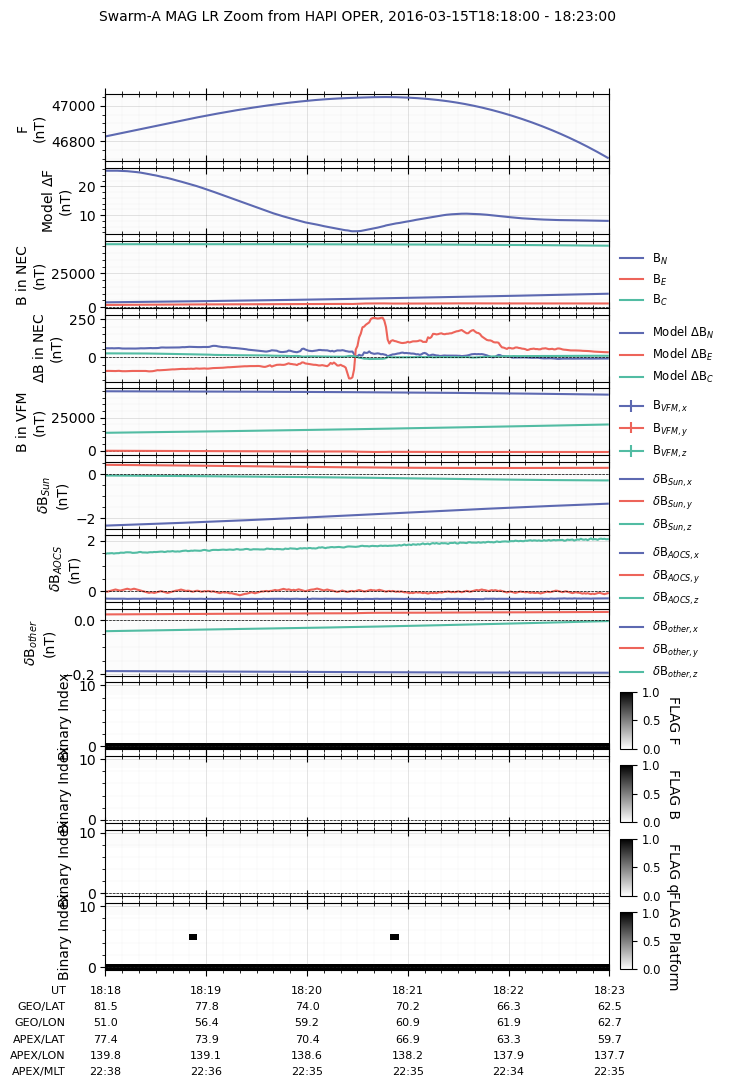
\includegraphics[width=0.7\linewidth]{files/b257be11371014259f98d2c0ca090599.png}

\subparagraph{Swarm MAG LR FAST from VirES HAPI service}

\begin{verbatim}
def test_swarm_MAG_LR_from_HAPI_FAST():
    """Test loading Swarm MAG LR data product from HAPI

    """
    dt_fr = datetime.datetime(2026, 3, 21, 18, 00)
    dt_to = datetime.datetime(2026, 3, 21, 18, 16)
    
    
    db = dashboards.TSDashboard(
        dt_fr=dt_fr, dt_to=dt_to, figure_config={'figsize': (8, 12)},
        timeline_extra_labels=['GEO_LAT', 'GEO_LON', 'APEX_LAT', 'APEX_LON', 'APEX_MLT',]  # Not applicable for very scattered data points like AEJ_PBS peaks
        )

    ds = db.dock(
        datasource_contents=['esa_eo', 'swarm', 'l1b', 'mag_lr'], 
        from_HAPI=True, from_FAST=True,
        sat_id='A', add_APEX=True,
    )

    panel_layouts = [
        [ds['F']],
        [ds['F_res_Model']],
        [ds['B_N'], ds['B_E'], ds['B_C']],
        [ds['B_res_Model_N'], ds['B_res_Model_E'], ds['B_res_Model_C']],
        [ds['B_VFM_x'], ds['B_VFM_y'], ds['B_VFM_z']],
        [ds['dB_Sun_VFM_x'], ds['dB_Sun_VFM_y'], ds['dB_Sun_VFM_z']],
        [ds['dB_AOCS_VFM_x'], ds['dB_AOCS_VFM_y'], ds['dB_AOCS_VFM_z']],
        [ds['dB_other_VFM_x'], ds['dB_other_VFM_y'], ds['dB_other_VFM_z']],
        [ds['FLAG_F_BIN_AUX']],
        [ds['FLAG_B_BIN_AUX']],
        [ds['FLAG_q_BIN_AUX']],
        [ds['FLAG_Platform_BIN_AUX']],
    ]

    db.set_layout(panel_layouts=panel_layouts)
    db.draw()
    db.add_title(title='Swarm -{} MAG LR Zoom from HAPI FAST'.format(ds.sat_id), fontsize='medium', append_time=True)
    
    db.save_figure(
        file_dir=file_dir_figure, 
        file_name='example_MAG_LR_Swarm -{}_zoom_HAPI_FAST'.format(ds.sat_id), 
        dpi=100, 
        append_time=False
    )
    db.show()
test_swarm_MAG_LR_from_HAPI_FAST()
\end{verbatim}

\begin{verbatim}
Create a new figure: Figure(800x1200).
INFO: Loading data from HAPI for server https://vires.services/hapi, dataset SW_FAST_MAGA_LR_1B, parameters Timestamp,Latitude,Longitude,Radius.
INFO: Data loaded from HAPI.
INFO: Loading data from HAPI for server https://vires.services/hapi, dataset SW_FAST_MAGA_LR_1B, parameters F,dF_Sun,dF_AOCS,dF_other,F_error,B_VFM,B_NEC,dB_Sun,dB_AOCS,dB_other,B_error.
INFO: Data loaded from HAPI.
INFO: Loading data from HAPI for server https://vires.services/hapi, dataset SW_FAST_MAGA_LR_1B, parameters q_NEC_CRF,Att_error,Flags_F,Flags_B,Flags_q,Flags_Platform,ASM_Freq_Dev.
INFO: Data loaded from HAPI.
INFO: Loading data from HAPI for server https://vires.services/hapi, dataset SW_FAST_MAGA_LR_1B, parameters SyncStatus,B_NEC_Model,F_Model,F_res_Model,B_NEC_res_Model.
INFO: Data loaded from HAPI.
WARNING: Variable CDF_EPOCH is not in the default variable names and does not match the patterns for automatically assigning configured variable names. It will be added without a configured variable name, and may not be included in the default panels for plotting and analysis. Please check if this variable should be included in the default variable names or if it follows the naming patterns for automatic assignment of configured variable names.
WARNING: Variable SC_GEO_R is not in the default variable names and does not match the patterns for automatically assigning configured variable names. It will be added without a configured variable name, and may not be included in the default panels for plotting and analysis. Please check if this variable should be included in the default variable names or if it follows the naming patterns for automatic assignment of configured variable names.
WARNING: Variable B_NEC_Model is not in the default variable names and does not match the patterns for automatically assigning configured variable names. It will be added without a configured variable name, and may not be included in the default panels for plotting and analysis. Please check if this variable should be included in the default variable names or if it follows the naming patterns for automatic assignment of configured variable names.
WARNING: Variable B_NEC_res_Model is not in the default variable names and does not match the patterns for automatically assigning configured variable names. It will be added without a configured variable name, and may not be included in the default panels for plotting and analysis. Please check if this variable should be included in the default variable names or if it follows the naming patterns for automatic assignment of configured variable names.
/opt/anaconda3/envs/Swarm/lib/python3.12/site -packages/numpy/_core/numeric.py:476: RuntimeWarning: invalid value encountered in cast
  multiarray.copyto(res, fill_value, casting='unsafe')
\end{verbatim}

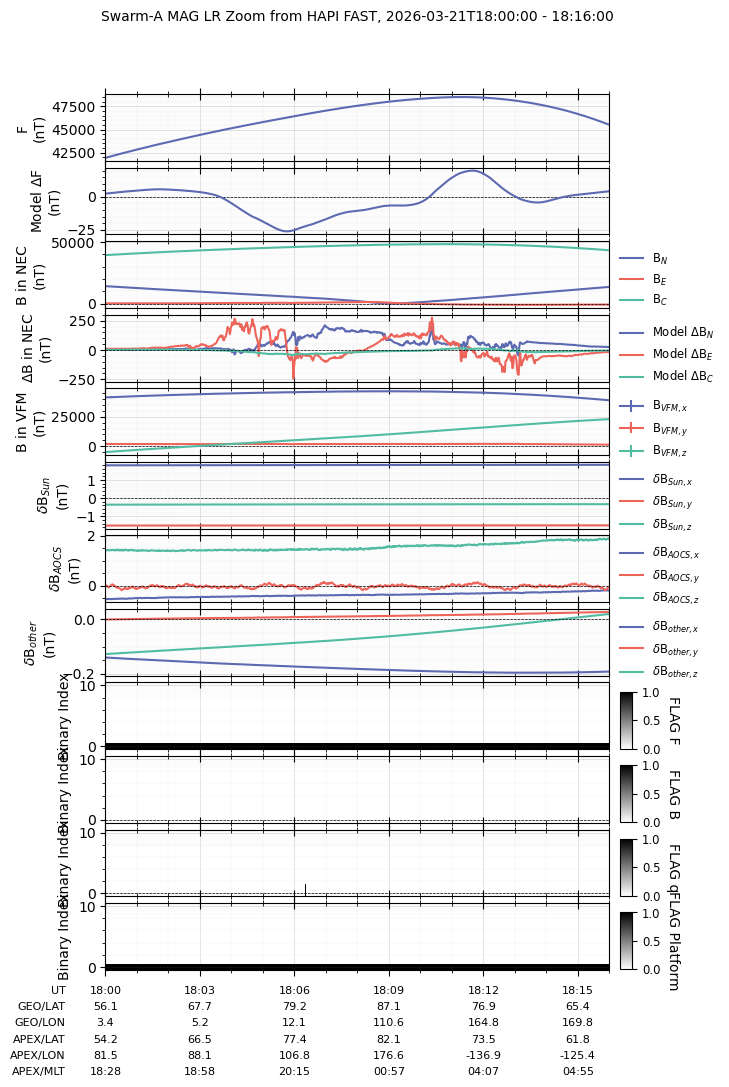
\includegraphics[width=0.7\linewidth]{files/46497c658e5cff4f2a98f37413cefedc.png}

\subsubsection{Swarm EFI LP and FP data products}

\begin{verbatim}
import datetime
import matplotlib.pyplot as plt
import numpy as np
import pathlib

import geospacelab.visualization.mpl.dashboards as dashboards
\end{verbatim}

\paragraph{Swarm EFI LP 1B data}

\begin{verbatim}
def test_swarm_EFI_LP_1B_overview():
    """Test Swarm EFI/LP 1B data product
    
    """
    dt_fr = datetime.datetime(2016, 3, 14, 20, 15)
    dt_to = datetime.datetime(2016, 3, 14, 21, 0)

    db = dashboards.TSDashboard(
        dt_fr=dt_fr, dt_to=dt_to, figure_config={'figsize': (8, 10)},
        timeline_extra_labels=['GEO_LAT', 'GEO_LON', 'APEX_LAT', 'APEX_LON', 'APEX_MLT'],
        )

    ds = db.dock(
        datasource_contents=['esa_eo', 'swarm', 'l1b', 'efi_lp'], 
        product_version='latest', # 'latest' (default),
        sat_id='A', add_APEX=True)
    ds.list_all_variables()
    
    panel_layouts = [
        [ds['n_i'], ds['n_e']],
        [ds['T_e']],
        [ds['V_SC']],
        [ds['FLAG_LP'], ds['FLAG_n_i'], ds['FLAG_n_e'], ds['FLAG_T_e'], ds['FLAG_V_SC']],
        [ds['FLAG_1_BIN_AUX'],],
        [ds['FLAG_2_BIN_AUX'],],
    ]
    # Change some default attrs for better visualization
    ds['T_e'].visual.axis[1].lim = [ -10, 10000]

    db.set_layout(panel_layouts=panel_layouts)
    db.draw()
    db.add_title(title='Swarm -{} EFI/LP 1B Overview'.format(ds.sat_id), fontsize='medium', append_time=True)

    db.show()
test_swarm_EFI_LP_1B_overview()
\end{verbatim}

\begin{verbatim}
Create a new figure: Figure(800x1000).
Searching the data product "EFI_LP" with the version "latest" on the server...
INFO: Indexing the files for the product EFI_LP of the satellite A ...
The file [PosixPath('/data/afys -ionosphere/data/ESA/SWARM/Level1b/EFI_LP/0701/Sat_A/2016/SW_OPER_EFIA_LP_1B_20160314T000000_20160314T235959_0701_MDR_EFI_LP.cdf')] already exists: skip downloading.
/opt/anaconda3/envs/Swarm/lib/python3.12/site -packages/numpy/_core/numeric.py:442: RuntimeWarning: invalid value encountered in cast
  multiarray.copyto(res, fill_value, casting='unsafe')
Dataset: esa/earthonline | swarm | efi | efi_lp
Printing all of the variables ...
|No.                 |Variable name                 |Variable name (Source)        |Description                                                                                         |
| - - - - - - - - - - - - - - - - - - - -| - - - - - - - - - - - - - - - - - - - - - - - - - - - - - -| - - - - - - - - - - - - - - - - - - - - - - - - - - - - - -| - - - - - - - - - - - - - - - - - - - - - - - - - - - - - - - - - - - - - - - - - - - - - - - - - - - - - - - - - - - - - - - - - - - - - - - - - - - - - - - - - - - - - - - - - - - - - - - - - - - -|
|1                   |SC_DATETIME                   |N/A                           |Time of observation                                                                                 |
|2                   |Sync_Status                   |SyncStatus                    |                                                                                                    |
|3                   |SC_GEO_LAT                    |Latitude                      |Geographic Latitude                                                                                 |
|4                   |SC_GEO_LON                    |Longitude                     |Geographic Longitude                                                                                |
|5                   |SC_GEO_r                      |N/A                           |                                                                                                    |
|6                   |v_SC_ITRF                     |U_orbit                       |S/C velocity in ITRF                                                                                |
|7                   |n_i                           |N_ion                         |Ion density                                                                                         |
|8                   |CALIB_n_i                     |dN_ion                        |Calibration parameter for n_i, wrt. ISRs                                                            |
|9                   |n_i_err                       |N_ion_error                   |                                                                                                    |
|10                  |n_e                           |N_elec                        |Electron density                                                                                    |
|11                  |n_e_err                       |N_elec_error                  |                                                                                                    |
|12                  |T_e                           |T_elec                        |Electron temperature                                                                                |
|13                  |T_e_err                       |T_elec_error                  |                                                                                                    |
|14                  |CALIB_T_e                     |dT_elec                       |Calibration parameter for T_e, wrt. ISRs                                                            |
|15                  |V_SC                          |Vs                            |S/C potential                                                                                       |
|16                  |V_SC_err                      |Vs_error                      |                                                                                                    |
|17                  |FLAG_LP                       |Flags_LP                      |Flag of source: 1, 5, 9                                                                             |
|18                  |FLAG_n_i                      |Flags_N_ion                   |Flag of n_i: 10 - 40                                                                                |
|19                  |FLAG_n_e                      |Flags_N_elec                  |Flag of n_e: 10 - 40                                                                                |
|20                  |FLAG_T_e                      |Flags_T_elec                  |Flag of T_e: 10 - 40                                                                                |
|21                  |FLAG_V_SC                     |Flags_Vs                      |Flag of V_SC: 20, 30                                                                                |
|22                  |FLAG_BITS_1                   |Flagbits1                     |Binary flag (Instrument)                                                                            |
|23                  |FLAG_BITS_2                   |Flagbits2                     |Binary flag (Gain)                                                                                  |
|24                  |FLAG_1_BIN_AUX                |N/A                           |Binary flag (Instrument)                                                                            |
|25                  |FLAG_2_BIN_AUX                |N/A                           |Binary flag (Gain)                                                                                  |
|26                  |FLAG_1_BIN_IND                |N/A                           |                                                                                                    |
|27                  |FLAG_2_BIN_IND                |N/A                           |                                                                                                    |
|28                  |Gamma_1                       |Gamma1                        |                                                                                                    |
|29                  |Gamma_2                       |Gamma2                        |                                                                                                    |
|30                  |SC_APEX_LAT                   |N/A                           |APEX Latitude                                                                                       |
|31                  |SC_APEX_LON                   |N/A                           |APEX Longitude                                                                                      |
|32                  |SC_APEX_MLT                   |N/A                           |APEX Magnetic Local Time                                                                            |
|33                  |SC_GEO_LST                    |N/A                           |Local Solar Time                                                                                    |
\end{verbatim}

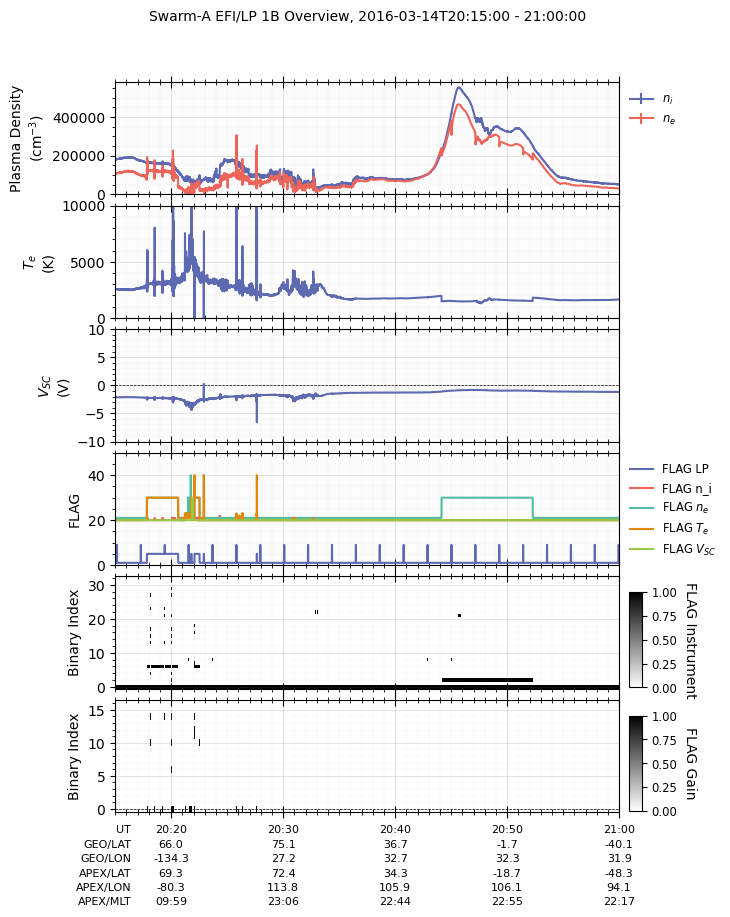
\includegraphics[width=0.7\linewidth]{files/0d82b0913aa228e966802f5e183f1ad5.png}

\paragraph{Swarm EFI LPI data}

\begin{verbatim}
def test_swarm_EFI_LPI_1B_overview():
    """Test Swarm EFI/LPI 1B data product
    
    """
    dt_fr = datetime.datetime(2016, 3, 14, 20, 15)
    dt_to = datetime.datetime(2016, 3, 14, 21, 0)

    db = dashboards.TSDashboard(
        dt_fr=dt_fr, dt_to=dt_to, figure_config={'figsize': (8, 10)},
        timeline_extra_labels=['GEO_LAT', 'GEO_LON', 'APEX_LAT', 'APEX_LON', 'APEX_MLT'],
        )

    ds = db.dock(
        datasource_contents=['esa_eo', 'swarm', 'l1b', 'efi_lpi'], 
        product_version='latest', # 'latest' (default),
        sat_id='A', add_APEX=True)
    
    panel_layouts = [
        [ds['n_i'], ds['n_e']],
        [ds['T_e']],
        [ds['V_SC']],
        [ds['FLAG_LP'], ds['FLAG_n_i'], ds['FLAG_n_e'], ds['FLAG_T_e'], ds['FLAG_V_SC']],
        [ds['FLAG_1_BIN_AUX'],],
        [ds['FLAG_2_BIN_AUX'],],
    ]
    # Change some default attrs for better visualization
    ds['T_e'].visual.axis[1].lim = [ -10, 10000]

    db.set_layout(panel_layouts=panel_layouts)
    db.draw()
    db.add_title(title='Swarm -{} EFI/LPI 1B Overview'.format(ds.sat_id), fontsize='medium', append_time=True)

    db.show()
test_swarm_EFI_LPI_1B_overview()
\end{verbatim}

\begin{verbatim}
Create a new figure: Figure(800x1000).
Searching the data product "EFI_LPI" with the version "latest" on the server...
The file [PosixPath('/data/afys -ionosphere/data/ESA/SWARM/Level1b/EFI_LPI/0701/Sat_A/2016/SW_OPER_EFIALPI_1B_20160314T000000_20160314T235959_0701_MDR_EFILPI.cdf')] already exists: skip downloading.
\end{verbatim}

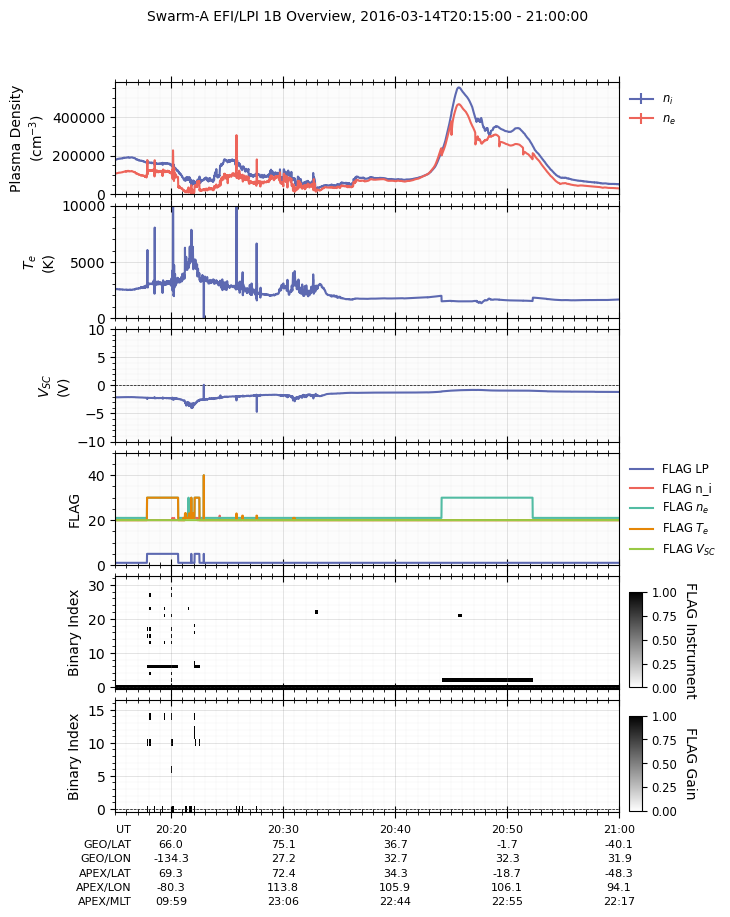
\includegraphics[width=0.7\linewidth]{files/834e3e20a3083951b5b314c059207316.png}

\paragraph{Swarm EFI LP FP data}

\begin{verbatim}
def test_swarm_EFI_LP_FP_overview():
    """Test Swarm EFI/LP -FP data product
    
    """
    dt_fr = datetime.datetime(2016, 3, 14, 20, 15)
    dt_to = datetime.datetime(2016, 3, 14, 21, 0)

    db = dashboards.TSDashboard(
        dt_fr=dt_fr, dt_to=dt_to, figure_config={'figsize': (8, 10)},
        timeline_extra_labels=['GEO_LAT', 'GEO_LON', 'APEX_LAT', 'APEX_LON', 'APEX_MLT'],
        )

    ds = db.dock(
        datasource_contents=['esa_eo', 'swarm', 'advanced', 'efi_lp_fp'], 
        product_version='latest', # 'latest' (default),
        sat_id='A', add_APEX=True)
    
    panel_layouts = [
        [ds['n_p']],
        [ds['I_FP']],
    ]
    
    db.set_layout(panel_layouts=panel_layouts)
    db.draw()
    db.add_title(title='Swarm -{} EFI/LP -FP Overview'.format(ds.sat_id), fontsize='medium', append_time=True)

    db.show()
test_swarm_EFI_LP_FP_overview()
\end{verbatim}

\begin{verbatim}
Create a new figure: Figure(800x1000).
Searching the data product "EFI_LP_FP" with the version "latest" on the server...
The file [PosixPath('/data/afys -ionosphere/data/ESA/SWARM/Advanced/EFI_LP_FP/0203/Sat_A/2016/SW_EXTD_EFIA_LP_FP_20160314T063806_20160314T235959_0203.cdf')] already exists: skip downloading.
\end{verbatim}

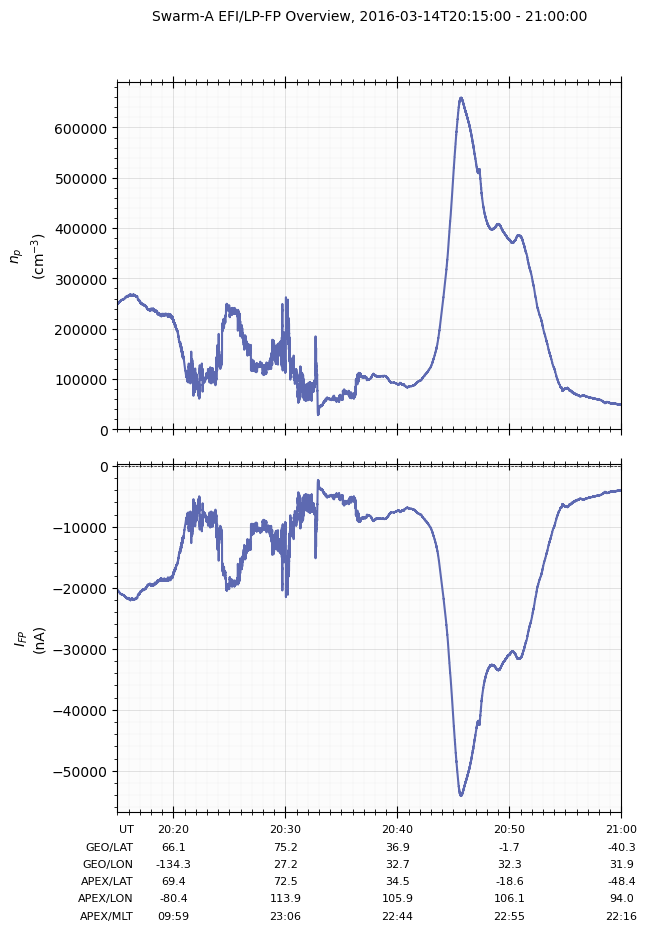
\includegraphics[width=0.7\linewidth]{files/fe18e90b6d1237b3afdce05e2aa707ae.png}

\paragraph{Swarm EFI LP HM data}

\begin{verbatim}
def test_swarm_EFI_LP_HM_overview():
    """Test Swarm EFI/LP -HM data product
    
    """
    dt_fr = datetime.datetime(2016, 3, 14, 20, 15)
    dt_to = datetime.datetime(2016, 3, 14, 21, 0)

    db = dashboards.TSDashboard(
        dt_fr=dt_fr, dt_to=dt_to, figure_config={'figsize': (8, 10)},
        timeline_extra_labels=['GEO_LAT', 'GEO_LON', 'APEX_LAT', 'APEX_LON', 'APEX_MLT'],
        )

    ds = db.dock(
        datasource_contents=['esa_eo', 'swarm', 'advanced', 'efi_lp_hm'], 
        product_version='latest', # 'latest' (default),
        sat_id='A', add_APEX=True)
    
    panel_layouts = [
        [ds['n_p']],
        [ds['T_e'], ds['T_e_HG'], ds['T_e_LG']],
        [ds['V_SC_HG'], ds['V_SC_LG']],
        [ds['FLAG_BIN_AUX'],],
    ]
    
    ds['T_e'].visual.axis[1].lim = [ -10, 10000]
    
    db.set_layout(panel_layouts=panel_layouts)
    db.draw()
    db.add_title(title='Swarm -{} EFI/LP -HM Overview'.format(ds.sat_id), fontsize='medium', append_time=True)

    db.show()
test_swarm_EFI_LP_HM_overview()
\end{verbatim}

\begin{verbatim}
Create a new figure: Figure(800x1000).
Searching the data product "EFI_LP_HM" with the version "latest" on the server...
The file [PosixPath('/data/afys -ionosphere/data/ESA/SWARM/Advanced/EFI_LP_HM/0102/Sat_A/2016/SW_EXTD_EFIA_LP_HM_20160314T000000_20160314T235959_0102.cdf')] already exists: skip downloading.
\end{verbatim}

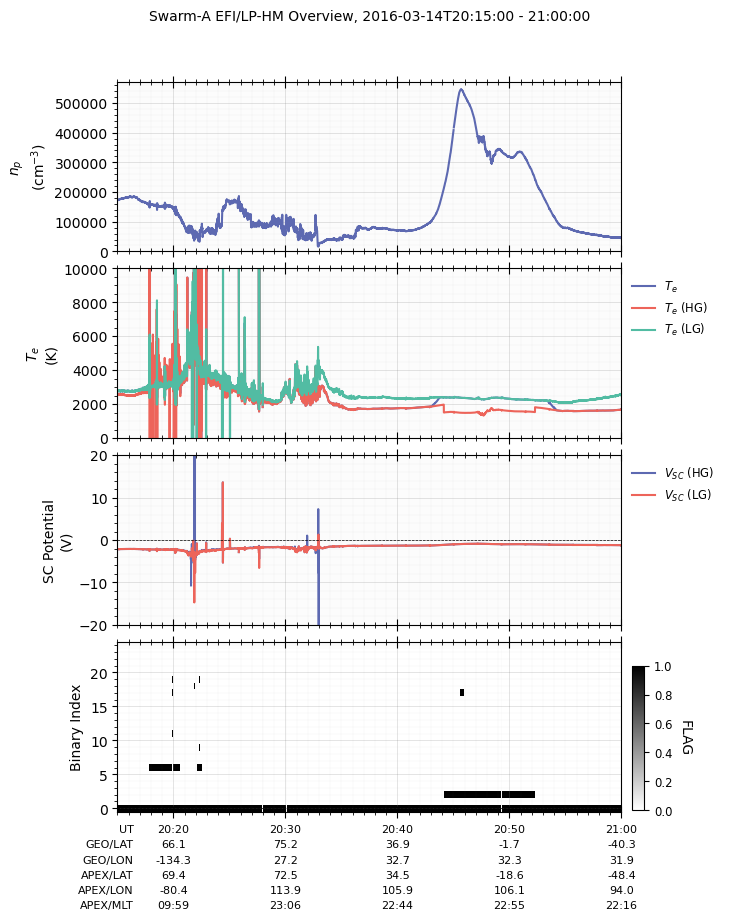
\includegraphics[width=0.7\linewidth]{files/f587d7fbc3a83824115bd14d99fb3623.png}

\paragraph{A combination of different EFI data products}

\begin{verbatim}
def test_swarm_compare_EFI_LP_FP_HM():
    """Test Swarm EFI/LP -FP vs. EFI/LP -HM data products
    
    """
    dt_fr = datetime.datetime(2016, 3, 14, 20, 15)
    dt_to = datetime.datetime(2016, 3, 14, 20, 35)

    db = dashboards.TSDashboard(
        dt_fr=dt_fr, dt_to=dt_to, figure_config={'figsize': (8, 10)},
        timeline_extra_labels=['GEO_LAT', 'GEO_LON', 'APEX_LAT', 'APEX_LON', 'APEX_MLT'],
        )

    ds_lp_fp = db.dock(
        datasource_contents=['esa_eo', 'swarm', 'advanced', 'efi_lp_fp'], 
        product_version='latest', # 'latest' (default),
        sat_id='A', add_APEX=True)
    
    ds_lp_1b = db.dock(
        datasource_contents=['esa_eo', 'swarm', 'l1b', 'efi_lp'], 
        product_version='latest', # 'latest' (default),
        sat_id='A', add_APEX=True)
    
    ds_lp_hm = db.dock(
        datasource_contents=['esa_eo', 'swarm', 'advanced', 'efi_lp_hm'], 
        product_version='latest', # 'latest' (default),
        sat_id='A', add_APEX=True)
    
    panel_layouts = [
        [ds_lp_fp['n_p'], ds_lp_1b['n_i'], ds_lp_1b['n_e'], ds_lp_hm['n_p']],
        [ds_lp_1b['T_e'], ds_lp_hm['T_e'], ds_lp_hm['T_e_HG'], ds_lp_hm['T_e_LG']],
        [ds_lp_1b['FLAG_LP'], ds_lp_1b['FLAG_n_i'], ds_lp_1b['FLAG_n_e'], ds_lp_1b['FLAG_T_e'], ds_lp_1b['FLAG_V_SC']],
        [ds_lp_1b['FLAG_1_BIN_AUX'],],
        [ds_lp_1b['FLAG_2_BIN_AUX'],],
        [ds_lp_hm['FLAG_BIN_AUX'],],
    ]
    ds_lp_1b['n_i'].visual.axis[2].label = r"n$_i$ (1B)"
    ds_lp_1b['n_e'].visual.axis[2].label = r"n$_e$ (1B)"
    ds_lp_1b['T_e'].visual.axis[2].label = r"T$_e$ (1B)"
    ds_lp_fp['n_p'].visual.axis[2].label = r"n$_p$ (FP)"
    ds_lp_hm['n_p'].visual.axis[2].label = r"n$_p$ (HM)"
    ds_lp_hm['T_e'].visual.axis[2].label = r"T$_e$ (HM)"
    ds_lp_hm['T_e_HG'].visual.axis[2].label = r"T$_e$ (HG)"
    ds_lp_hm['T_e_LG'].visual.axis[2].label = r"T$_e$ (LG)"
    ds_lp_1b['T_e'].visual.axis[1].lim = [ -10, 10000]
    
    db.set_layout(panel_layouts=panel_layouts)
    db.draw()
    db.add_title(title='Swarm -{} EFI/LP 1B vs FP vs HM Comparison'.format(ds_lp_fp.sat_id), fontsize='medium', append_time=True)

    db.show()
test_swarm_compare_EFI_LP_FP_HM()
\end{verbatim}

\begin{verbatim}
Create a new figure: Figure(800x1000).
Searching the data product "EFI_LP_FP" with the version "latest" on the server...
The file [PosixPath('/data/afys -ionosphere/data/ESA/SWARM/Advanced/EFI_LP_FP/0203/Sat_A/2016/SW_EXTD_EFIA_LP_FP_20160314T063806_20160314T235959_0203.cdf')] already exists: skip downloading.
Searching the data product "EFI_LP" with the version "latest" on the server...
The file [PosixPath('/data/afys -ionosphere/data/ESA/SWARM/Level1b/EFI_LP/0701/Sat_A/2016/SW_OPER_EFIA_LP_1B_20160314T000000_20160314T235959_0701_MDR_EFI_LP.cdf')] already exists: skip downloading.
Searching the data product "EFI_LP_HM" with the version "latest" on the server...
The file [PosixPath('/data/afys -ionosphere/data/ESA/SWARM/Advanced/EFI_LP_HM/0102/Sat_A/2016/SW_EXTD_EFIA_LP_HM_20160314T000000_20160314T235959_0102.cdf')] already exists: skip downloading.
\end{verbatim}

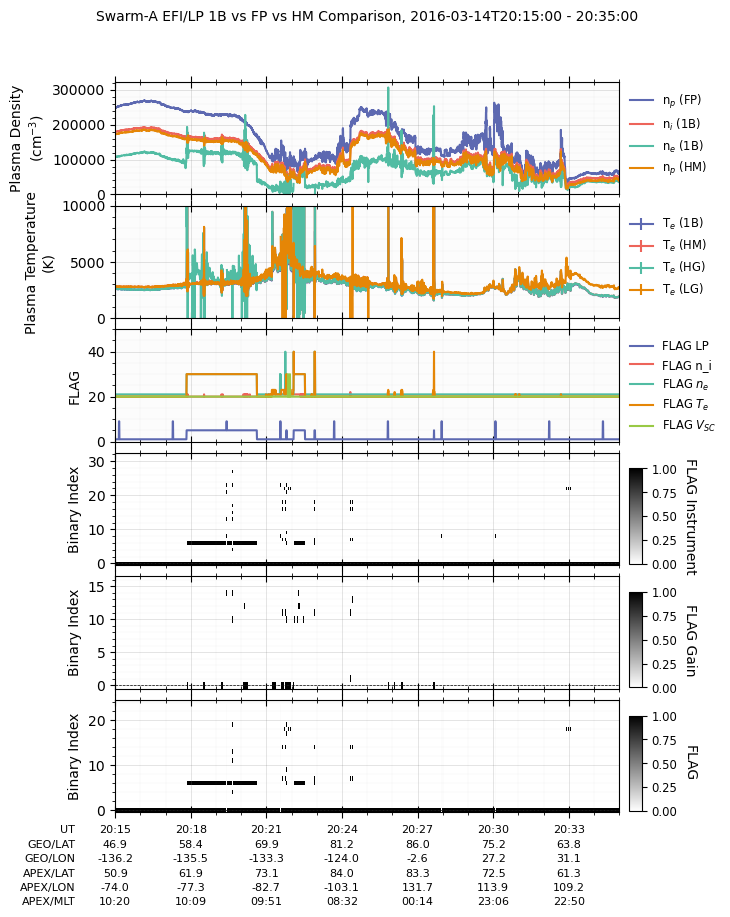
\includegraphics[width=0.7\linewidth]{files/0414ee2df957691c9b6bdbb1e8c5dd9b.png}

\subsubsection{Swarm EFI TII TCT data products}

\begin{verbatim}
import datetime
import matplotlib.pyplot as plt
import numpy as np
import pathlib
import os

import geospacelab.visualization.mpl.dashboards as dashboards

cwd = pathlib.Path(os.path.abspath(''))
file_dir_figure = cwd / 'figures'
file_dir_figure.mkdir(parents=True, exist_ok=True)
\end{verbatim}

\paragraph{Swarm EFI TII TCT 2Hz data}

\subparagraph{Overview with a long time span}

\begin{verbatim}
def test_swarm_EFI_TII_TCT02_overview():
    """Test Swarm EFI TII TCT02 data product
    
    """
    dt_fr = datetime.datetime(2015, 3, 17, 8, 0)
    dt_to = datetime.datetime(2015, 3, 17, 18, 0)

    db = dashboards.TSDashboard(
        dt_fr=dt_fr, dt_to=dt_to, figure_config={'figsize': (8, 12)},
        )

    ds = db.dock(datasource_contents=['esa_eo', 'swarm', 'advanced', 'efi_tct02'], sat_id='A', add_APEX=True,)

    panel_layouts = [
        [ds['v_i_H_x'], ds['v_i_V_x'], ds['v_i_H_y'], ds['v_i_V_z']],
        [ds['v_SC_N'], ds['v_SC_E'], ds['v_SC_C']],
        [ds['E_H_x'], ds['E_H_y'], ds['E_H_z']],
        [ds['E_V_x'], ds['E_V_y'], ds['E_V_z']],
        [ds['B_x'], ds['B_y'], ds['B_z']],
        [ds['v_i_CR_x'], ds['v_i_CR_y'], ds['v_i_CR_z']],
        [ds['QUALITY_FLAG_BIN_AUX'],],
        [ds['CALIB_FLAG_BIN_AUX'],],
    ]

    db.set_layout(panel_layouts=panel_layouts)
    db.draw()
    db.add_title(title='Swarm -{} EFI TII TCT02 Overview'.format(ds.sat_id), fontsize='medium', append_time=True)

    db.save_figure(
        file_dir=file_dir_figure, 
        file_name='example_EFI_TII_TCT02_Swarm -{}_overview'.format(ds.sat_id), 
        dpi=100, 
        append_time=False)
    db.show()
test_swarm_EFI_TII_TCT02_overview()
\end{verbatim}

\begin{verbatim}
Create a new figure: Figure(800x1200).
\end{verbatim}

\begin{verbatim}
Load IGRF coefficients ...
\end{verbatim}

\begin{verbatim}
Searching the data product "EFI_TCT02" with the version "latest" on the server...
The file [PosixPath('/data/afys -ionosphere/data/ESA/SWARM/Advanced/EFI_TII/TCT02/0401/Sat_A/2015/SW_EXPT_EFIA_TCT02_20150317T000000_20150317T235959_0401.cdf')] already exists: skip downloading.
/opt/anaconda3/envs/Swarm/lib/python3.12/site -packages/numpy/_core/numeric.py:476: RuntimeWarning: invalid value encountered in cast
  multiarray.copyto(res, fill_value, casting='unsafe')
\end{verbatim}

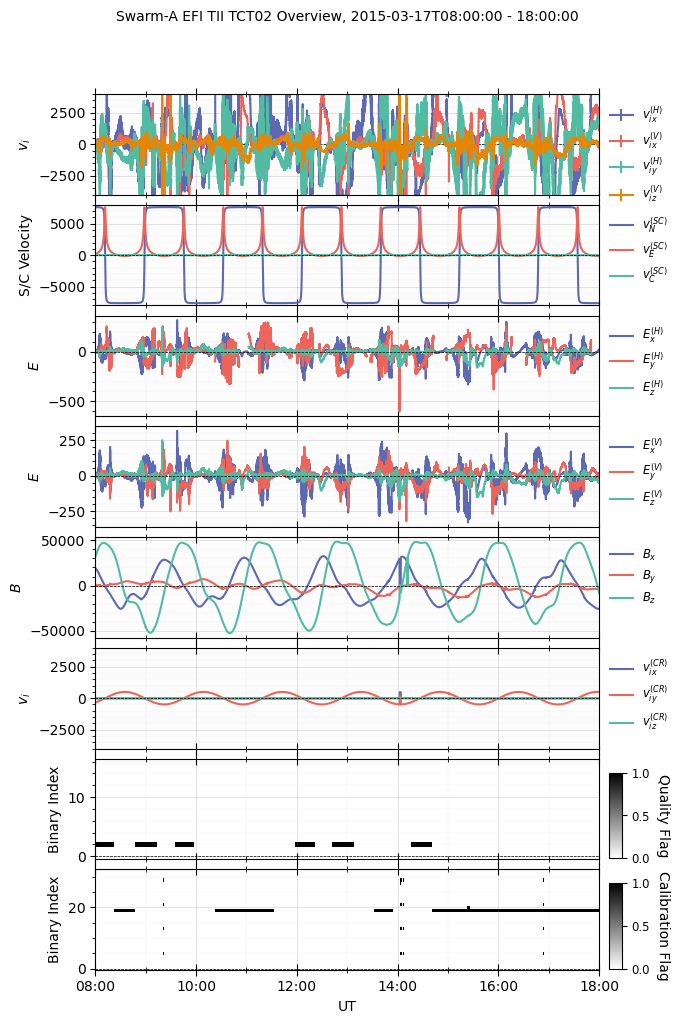
\includegraphics[width=0.7\linewidth]{files/f9b76a8bfab2158b755e845ae5b41e4f.png}

\subparagraph{Zoomed-in with a short time span}

\begin{verbatim}
def test_swarm_EFI_TII_TCT02_zoom():
    """Test Swarm EFI TII TCT02 data product
    
    """
    dt_fr = datetime.datetime(2015, 3, 17, 12, 40)
    dt_to = datetime.datetime(2015, 3, 17, 13, 10)

    db = dashboards.TSDashboard(
        dt_fr=dt_fr, dt_to=dt_to, figure_config={'figsize': (8, 12)},
        # timeline_extra_labels=['GEO_LAT', 'GEO_LON', 'APEX_LAT', 'APEX_LON', 'APEX_MLT',]  # Not applicable for very scattered data points like AEJ_PBS peaks
        )

    ds = db.dock(datasource_contents=['esa_eo', 'swarm', 'advanced', 'efi_tct02'], sat_id='A', add_APEX=True,)

    panel_layouts = [
        [ds['v_i_H_x'], ds['v_i_V_x'], ds['v_i_H_y'], ds['v_i_V_z']],
        [ds['v_SC_N'], ds['v_SC_E'], ds['v_SC_C']],
        [ds['E_H_x'], ds['E_H_y'], ds['E_H_z']],
        [ds['E_V_x'], ds['E_V_y'], ds['E_V_z']],
        [ds['B_x'], ds['B_y'], ds['B_z']],
        [ds['v_i_CR_x'], ds['v_i_CR_y'], ds['v_i_CR_z']],
        [ds['QUALITY_FLAG_BIN_AUX'],],
        [ds['CALIB_FLAG_BIN_AUX'],],
    ]

    db.set_layout(panel_layouts=panel_layouts)
    db.draw()
    db.add_title(title='Swarm -{} EFI TII TCT02 Zoom'.format(ds.sat_id), fontsize='medium', append_time=True)
    
    db.save_figure(
        file_dir=file_dir_figure, 
        file_name='example_EFI_TII_TCT02_Swarm -{}_zoom'.format(ds.sat_id), 
        dpi=100, 
        append_time=False)
    db.show()
test_swarm_EFI_TII_TCT02_zoom()
\end{verbatim}

\begin{verbatim}
Create a new figure: Figure(800x1200).
Searching the data product "EFI_TCT02" with the version "latest" on the server...
The file [PosixPath('/data/afys -ionosphere/data/ESA/SWARM/Advanced/EFI_TII/TCT02/0401/Sat_A/2015/SW_EXPT_EFIA_TCT02_20150317T000000_20150317T235959_0401.cdf')] already exists: skip downloading.
\end{verbatim}

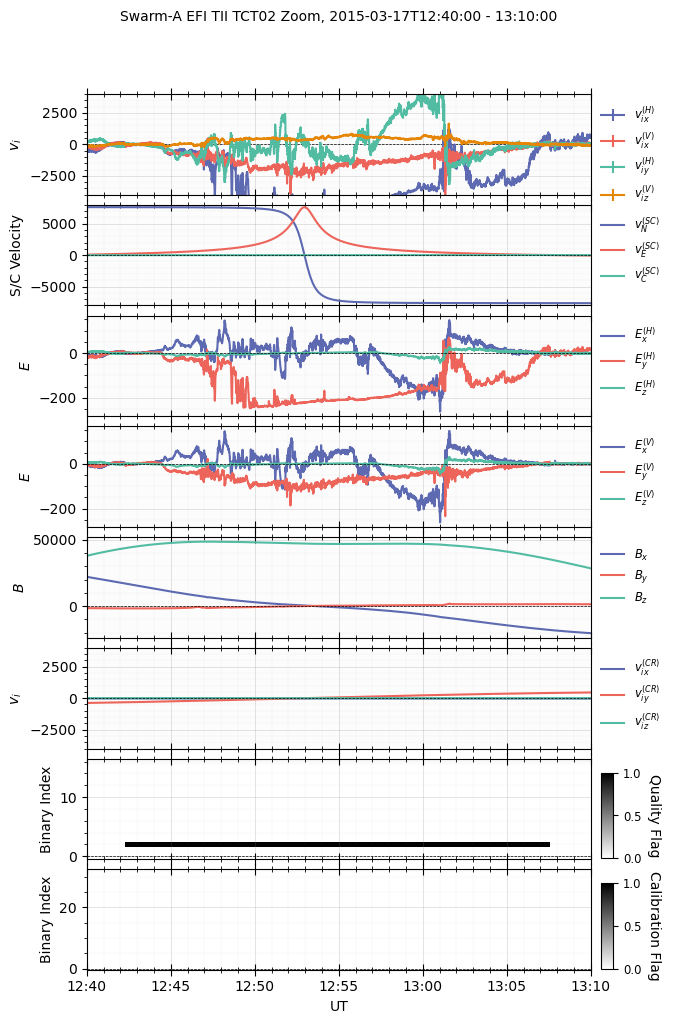
\includegraphics[width=0.7\linewidth]{files/2ba6d5416cf4759ee3511ffcecab9d58.png}

\paragraph{Swarm EFI TII TCT 16 Hz data}

\begin{verbatim}
def test_swarm_EFI_TII_TCT16_zoom():
    """Test Swarm EFI TII TCT16 data product
    
    """
    dt_fr = datetime.datetime(2015, 3, 17, 12, 40)
    dt_to = datetime.datetime(2015, 3, 17, 13, 10)

    db = dashboards.TSDashboard(
        dt_fr=dt_fr, dt_to=dt_to, figure_config={'figsize': (8, 12)},
        )

    ds = db.dock(datasource_contents=['esa_eo', 'swarm', 'advanced', 'efi_tct16'], sat_id='A', add_APEX=True,)

    panel_layouts = [
        [ds['v_i_H_x'], ds['v_i_V_x'], ds['v_i_H_y'], ds['v_i_V_z']],
        [ds['v_SC_N'], ds['v_SC_E'], ds['v_SC_C']],
        [ds['E_H_x'], ds['E_H_y'], ds['E_H_z']],
        [ds['E_V_x'], ds['E_V_y'], ds['E_V_z']],
        [ds['B_x'], ds['B_y'], ds['B_z']],
        [ds['v_i_CR_x'], ds['v_i_CR_y'], ds['v_i_CR_z']],
        [ds['QUALITY_FLAG_BIN_AUX'],],
        [ds['CALIB_FLAG_BIN_AUX'],],
    ]

    db.set_layout(panel_layouts=panel_layouts)
    db.draw()
    db.add_title(title='Swarm -{} EFI TII TCT16 Zoom'.format(ds.sat_id), fontsize='medium', append_time=True)

    db.save_figure(
        file_dir=file_dir_figure, 
        file_name='example_EFI_TII_TCT16_Swarm -{}_zoom'.format(ds.sat_id), 
        dpi=100, 
        append_time=False)
    db.show()
test_swarm_EFI_TII_TCT16_zoom()
\end{verbatim}

\begin{verbatim}
Create a new figure: Figure(800x1200).
Searching the data product "EFI_TCT16" with the version "latest" on the server...
INFO: Indexing the files for the product EFI_TCT16 of the satellite A ...
The file [PosixPath('/data/afys -ionosphere/data/ESA/SWARM/Advanced/EFI_TII/TCT16/0401/Sat_A/2015/SW_EXPT_EFIA_TCT16_20150317T000000_20150317T235959_0401.cdf')] already exists: skip downloading.
\end{verbatim}

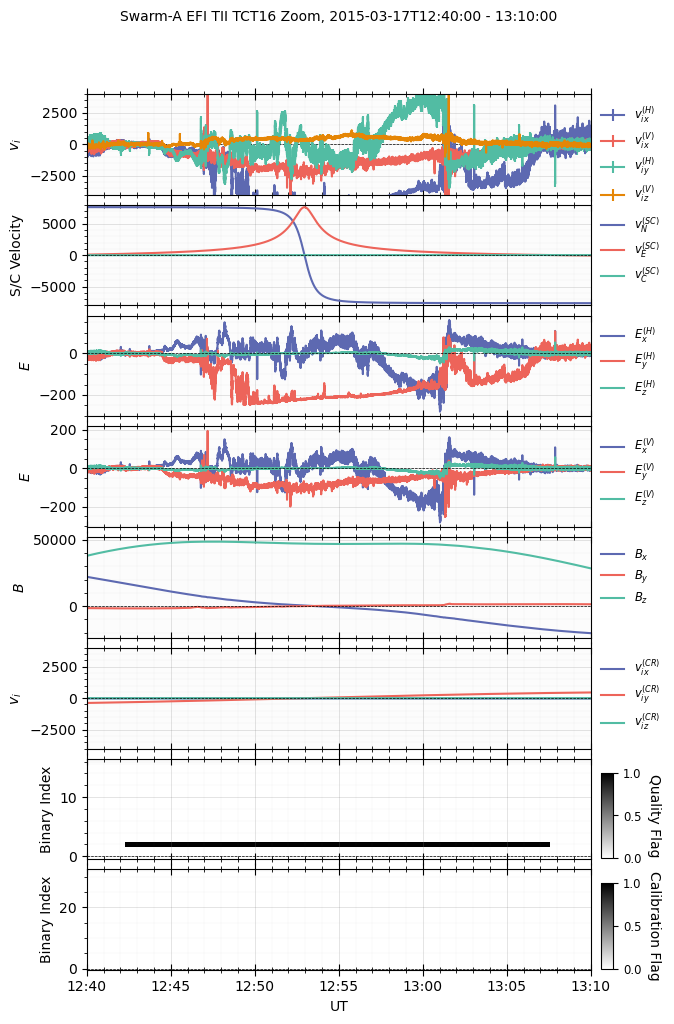
\includegraphics[width=0.7\linewidth]{files/aecc506c2c2541c2bb5e2a9264136729.png}

\subsubsection{Swarm EFI IDM data product}

\begin{verbatim}
import datetime
import pathlib
import os

import geospacelab.visualization.mpl.dashboards as dashboards

cwd = pathlib.Path(os.path.abspath(''))
file_dir_figure = cwd / 'figures'
file_dir_figure.mkdir(parents=True, exist_ok=True)
\end{verbatim}

\paragraph{Overview}

\begin{verbatim}
def test_swarm_EFI_IDM_overview():
    """Test Swarm EFI IDM data product
    
    """
    dt_fr = datetime.datetime(2016, 3, 14, 15, 0)
    dt_to = datetime.datetime(2016, 3, 14, 22, 0)

    db = dashboards.TSDashboard(
        dt_fr=dt_fr, dt_to=dt_to, figure_config={'figsize': (8, 12)},
        )

    ds = db.dock(datasource_contents=['esa_eo', 'swarm', 'advanced', 'efi_idm'], sat_id='A', add_APEX=True,)

    panel_layouts = [
        [ds['M_i_eff_model'], ds['M_i_eff']],
        [ds['FLAG_M_i_eff_BIN_AUX']],
        [ds['v_i_raw'], ds['v_i']],
        [ds['FLAG_v_i_BIN_AUX']],
        [ds['n_i'],],
        [ds['FLAG_n_i_BIN_AUX']],
    ]

    db.set_layout(panel_layouts=panel_layouts)
    db.draw()
    db.add_title(title='Swarm -{} EFI IDM Overview'.format(ds.sat_id), fontsize='medium', append_time=True)

    db.save_figure(file_dir=file_dir_figure, file_name='example_EFI_IDM_Swarm -{}_overview'.format(ds.sat_id), dpi=100, append_time=False)
    db.show()
test_swarm_EFI_IDM_overview()
\end{verbatim}

\begin{verbatim}
Create a new figure: Figure(800x1200).
\end{verbatim}

\begin{verbatim}
Load IGRF coefficients ...
\end{verbatim}

\begin{verbatim}
Searching the data product "EFI_IDM" with the version "latest" on the server...
INFO: Indexing the files for the product EFI_IDM of the satellite A ...
The file [PosixPath('/data/afys -ionosphere/data/ESA/SWARM/Advanced/EFI_IDM/0301/Sat_A/2016/SW_PREL_EFIAIDM_2__20160314T000000_20160314T235959_0301.cdf')] already exists: skip downloading.
/opt/anaconda3/envs/Swarm/lib/python3.12/site -packages/numpy/_core/numeric.py:476: RuntimeWarning: invalid value encountered in cast
  multiarray.copyto(res, fill_value, casting='unsafe')
\end{verbatim}

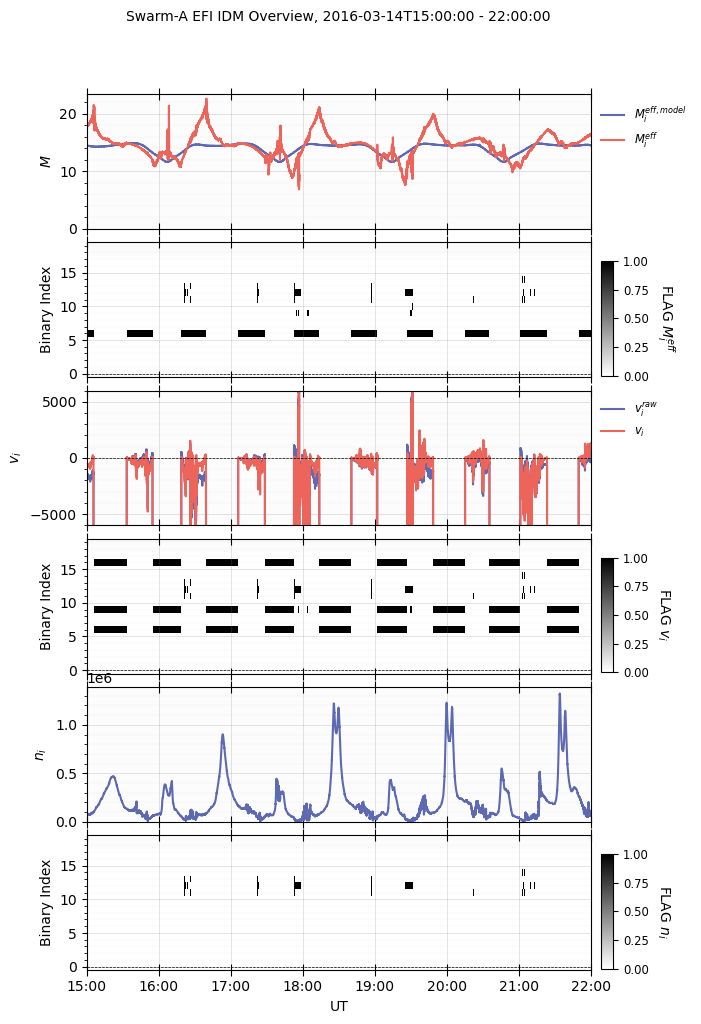
\includegraphics[width=0.7\linewidth]{files/cbb5f9cd4d3ec654585a4e93663df226.png}

\paragraph{Zoomed-in}

\begin{verbatim}
def test_swarm_EFI_IDM_zoom():
    """Test Swarm EFI IDM data product
    
    """
    dt_fr = datetime.datetime(2016, 3, 14, 20, 15)
    dt_to = datetime.datetime(2016, 3, 14, 21, 0)

    db = dashboards.TSDashboard(
        dt_fr=dt_fr, dt_to=dt_to, figure_config={'figsize': (8, 12)},
        timeline_extra_labels=['GEO_LAT', 'GEO_LON', 'APEX_LAT', 'APEX_LON', 'APEX_MLT',]  # Not applicable for very scattered data points like AEJ_PBS peaks
        )

    ds = db.dock(datasource_contents=['esa_eo', 'swarm', 'advanced', 'efi_idm'], sat_id='A', add_APEX=True,)

    panel_layouts = [
        [ds['M_i_eff_model'], ds['M_i_eff']],
        [ds['FLAG_M_i_eff_BIN_AUX']],
        [ds['v_i_raw'], ds['v_i']],
        [ds['FLAG_v_i_BIN_AUX']],
        [ds['n_i'],],
        [ds['FLAG_n_i_BIN_AUX']],
    ]

    db.set_layout(panel_layouts=panel_layouts)
    db.draw()
    db.add_title(title='Swarm -{} EFI IDM Zoom'.format(ds.sat_id), fontsize='medium', append_time=True)
    
    db.save_figure(file_dir=file_dir_figure, file_name='example_EFI_IDM_Swarm -{}_zoom'.format(ds.sat_id), dpi=100, append_time=False)
    db.show()
test_swarm_EFI_IDM_zoom()
\end{verbatim}

\begin{verbatim}
Create a new figure: Figure(800x1200).
Searching the data product "EFI_IDM" with the version "latest" on the server...
The file [PosixPath('/data/afys -ionosphere/data/ESA/SWARM/Advanced/EFI_IDM/0301/Sat_A/2016/SW_PREL_EFIAIDM_2__20160314T000000_20160314T235959_0301.cdf')] already exists: skip downloading.
\end{verbatim}

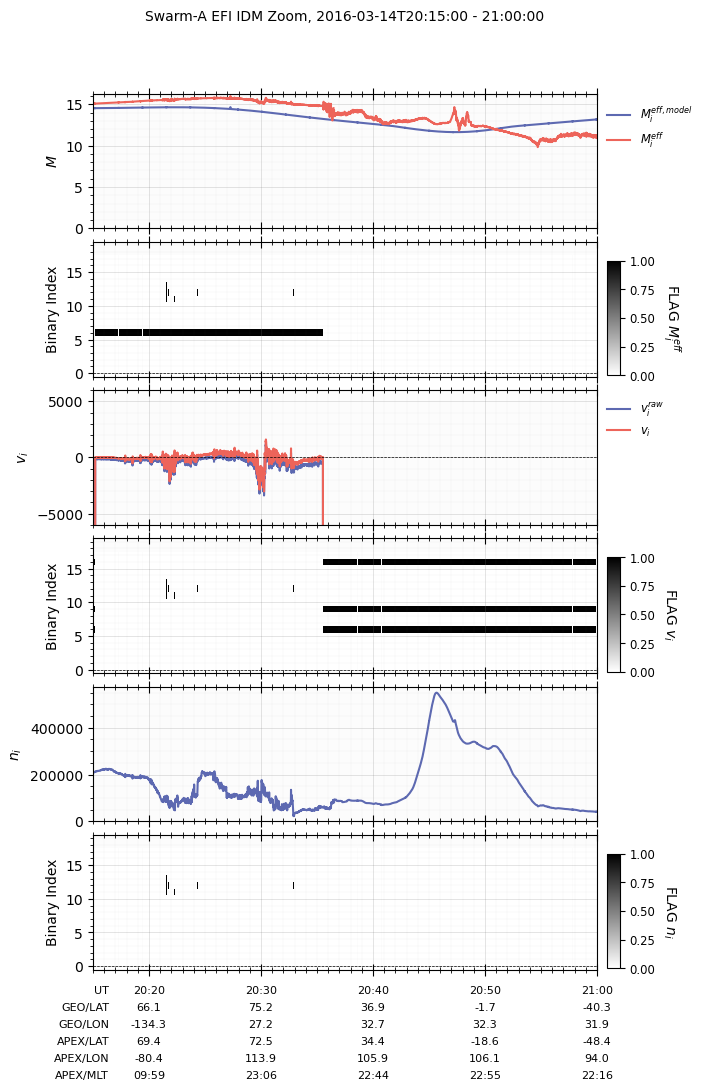
\includegraphics[width=0.7\linewidth]{files/350886159281263ffac87c6711a10f83.png}

\subsubsection{Swarm AEJ data products}

\begin{verbatim}
import datetime
import matplotlib.pyplot as plt
import numpy as np
import pathlib

import geospacelab.visualization.mpl.dashboards as dashboards
\end{verbatim}

\paragraph{Swarm AEJ LPS data product}

\subparagraph{Overview with a long time span}

\begin{verbatim}
def test_swarm_AEJ_LPL_overview():
    """Test Swarm AEJ/LPL data product
    
    """
    dt_fr = datetime.datetime(2024, 5, 10, 12, 0)
    dt_to = datetime.datetime(2024, 5, 11, 12, 0)

    db = dashboards.TSDashboard(
        dt_fr=dt_fr, dt_to=dt_to, figure_config={'figsize': (8, 8)},
        )

    ds = db.dock(
        datasource_contents=['esa_eo', 'swarm', 'l2daily', 'aej_lpl'], 
        product_version='latest', # 'latest' (default), '0301', 
        sat_id='C', add_APEX=True, add_AACGM=True)

    glat = ds['GEO_LAT']
    glon = ds['GEO_LON']
    J_N = ds['J_N']
    J_E = ds['J_E']
    J_QD = ds['J_QD']
    
    panel_layouts = [
        [J_N, J_E],
        [J_QD],
        [glat, [glon]]
    ]

    db.set_layout(panel_layouts=panel_layouts)
    db.draw()
    db.add_title(title='Swarm -{} AEJ/LPL Overview'.format(ds.sat_id), fontsize='medium', append_time=True)

    db.show()
    
test_swarm_AEJ_LPL_overview()
\end{verbatim}

\begin{verbatim}
Create a new figure: Figure(800x800).
\end{verbatim}

\begin{verbatim}
Load IGRF coefficients ...
\end{verbatim}

\begin{verbatim}
Searching the data product "AEJ_LPL" with the version "latest" on the server...
INFO: Indexing the files for the product AEJ_LPL of the satellite C ...
The file [PosixPath('/data/afys -ionosphere/data/ESA/SWARM/Level2daily/AEJ_LPL/0301/Sat_C/2024/SW_OPER_AEJCLPL_2F_20240510T000000_20240510T235959_0301.cdf')] already exists: skip downloading.
The file [PosixPath('/data/afys -ionosphere/data/ESA/SWARM/Level2daily/AEJ_LPL/0301/Sat_C/2024/SW_OPER_AEJCLPL_2F_20240511T000000_20240511T235959_0301.cdf')] already exists: skip downloading.
resetting environment variable IGRF_COEFFS in python script
resetting environment variable AACGM_v2_DAT_PREFIX in python script
non -default coefficient files may be specified by running aacgmv2.wrapper.set_coeff_path before any other functions
/opt/anaconda3/envs/Swarm/lib/python3.12/site -packages/numpy/_core/numeric.py:476: RuntimeWarning: invalid value encountered in cast
  multiarray.copyto(res, fill_value, casting='unsafe')
\end{verbatim}

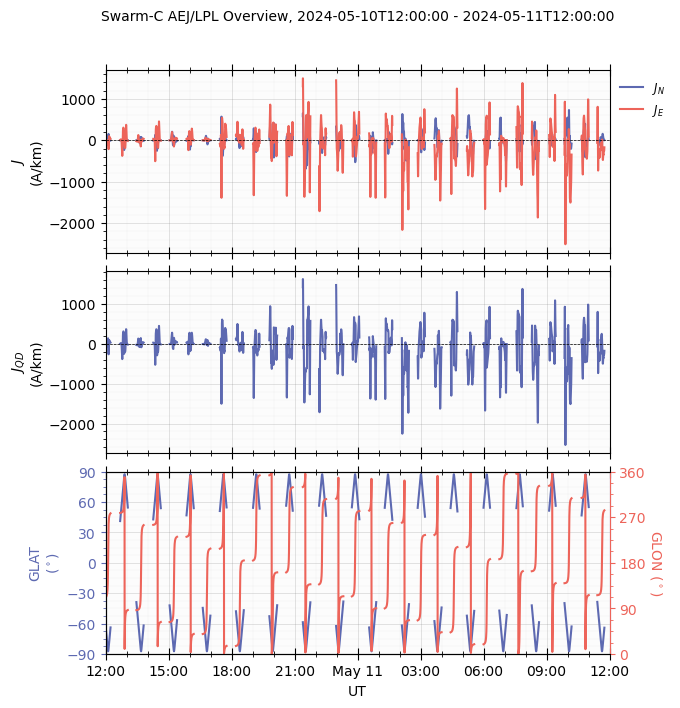
\includegraphics[width=0.7\linewidth]{files/395de7af547d1f43c3c00947d4da195a.png}

\subparagraph{Zoomed-in view with a short time span}

\begin{verbatim}
def test_swarm_AEJ_LPL_zoom():
    """Test Swarm AEJ/LPL data product
    
    """
    dt_fr = datetime.datetime(2024, 5, 10, 20, 30)
    dt_to = datetime.datetime(2024, 5, 10, 21, 0)

    db = dashboards.TSDashboard(
        dt_fr=dt_fr, dt_to=dt_to, figure_config={'figsize': (8, 8)},
        timeline_extra_labels=['GEO_LAT', 'GEO_LON', 'APEX_LAT', 'APEX_LON', 'APEX_MLT',] 
        )

    ds = db.dock(datasource_contents=['esa_eo', 'swarm', 'l2daily', 'aej_lpl'], sat_id='C', add_APEX=True, add_AACGM=True)

    glat = ds['GEO_LAT']
    glon = ds['GEO_LON']
    J_N = ds['J_N']
    J_E = ds['J_E']
    J_QD = ds['J_QD']
    
    panel_layouts = [
        [J_N, J_E],
        [J_QD],
        [glat, [glon]]
    ]

    db.set_layout(panel_layouts=panel_layouts)
    db.draw()
    db.add_title(title='Swarm -{} AEJ/LPL Zoom'.format(ds.sat_id), fontsize='medium', append_time=True)
    
    db.show()
test_swarm_AEJ_LPL_zoom()
\end{verbatim}

\begin{verbatim}
Create a new figure: Figure(800x800).
Searching the data product "AEJ_LPL" with the version "latest" on the server...
The file [PosixPath('/data/afys -ionosphere/data/ESA/SWARM/Level2daily/AEJ_LPL/0301/Sat_C/2024/SW_OPER_AEJCLPL_2F_20240510T000000_20240510T235959_0301.cdf')] already exists: skip downloading.
\end{verbatim}

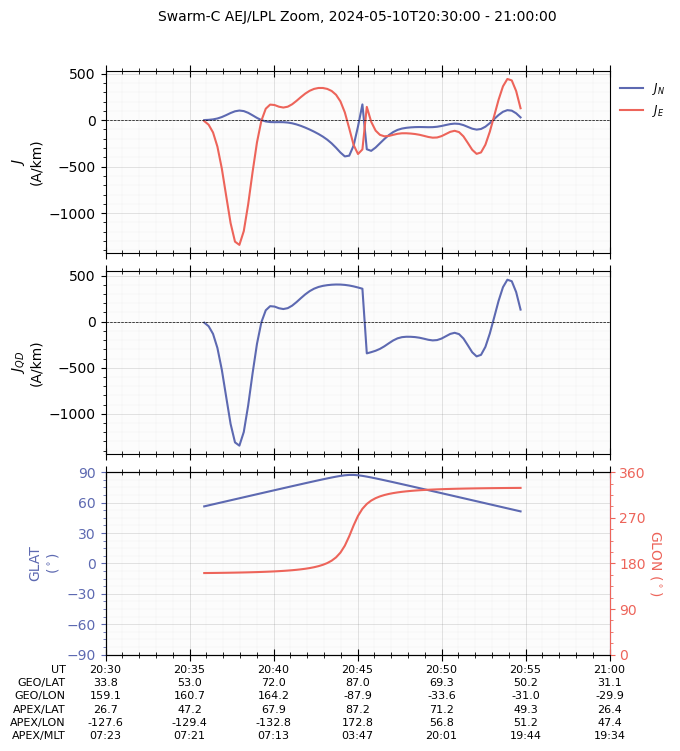
\includegraphics[width=0.7\linewidth]{files/a3e38009b0b655142392719442c30737.png}

\paragraph{Swarm AEJ LPS data product}

\subparagraph{Overview with a long time span}

\begin{verbatim}
def test_swarm_AEJ_LPS_overview():
    """Test Swarm AEJ/LPS data product
    
    """
    dt_fr = datetime.datetime(2024, 5, 10, 12, 0)
    dt_to = datetime.datetime(2024, 5, 11, 12, 0)

    db = dashboards.TSDashboard(
        dt_fr=dt_fr, dt_to=dt_to, figure_config={'figsize': (8, 8)},
        )

    ds = db.dock(datasource_contents=['esa_eo', 'swarm', 'l2daily', 'aej_lps'], sat_id='C', add_APEX=True, add_AACGM=True)

    glat = ds['GEO_LAT']
    glon = ds['GEO_LON']
    J_CF_N = ds['J_CF_N']
    J_CF_E = ds['J_CF_E']
    J_DF_N = ds['J_DF_N']
    J_DF_E = ds['J_DF_E']
    J_r = ds['J_r']
    
    panel_layouts = [
        [J_CF_N, J_CF_E],
        [J_DF_N, J_DF_E],
        [J_r],
        [glat, [glon]]
    ]

    db.set_layout(panel_layouts=panel_layouts)
    db.draw()
    db.add_title(title='Swarm -{} AEJ/LPS Overview'.format(ds.sat_id), fontsize='medium', append_time=True)

    db.show()
test_swarm_AEJ_LPS_overview()
\end{verbatim}

\begin{verbatim}
Create a new figure: Figure(800x800).
Searching the data product "AEJ_LPS" with the version "latest" on the server...
INFO: Indexing the files for the product AEJ_LPS of the satellite C ...
The file [PosixPath('/data/afys -ionosphere/data/ESA/SWARM/Level2daily/AEJ_LPS/0101/Sat_C/2024/SW_OPER_AEJCLPS_2F_20240510T000000_20240510T235959_0101.cdf')] already exists: skip downloading.
The file [PosixPath('/data/afys -ionosphere/data/ESA/SWARM/Level2daily/AEJ_LPS/0101/Sat_C/2024/SW_OPER_AEJCLPS_2F_20240511T000000_20240511T235959_0101.cdf')] already exists: skip downloading.
\end{verbatim}

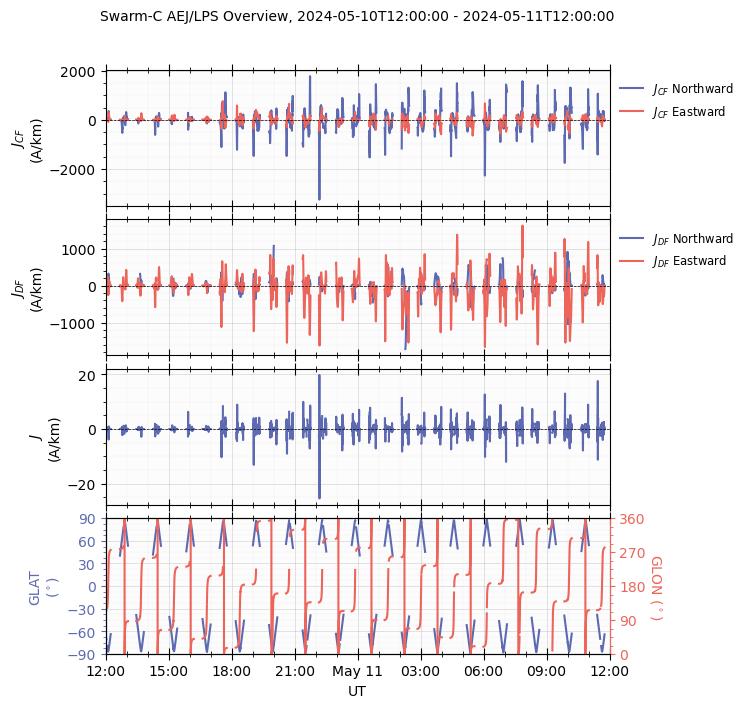
\includegraphics[width=0.7\linewidth]{files/82eb2efe96a89c248afb93adecff475f.png}

\subparagraph{Zoomed-in view with a short time span}

\begin{verbatim}
def test_swarm_AEJ_LPS_zoom():
    """Test Swarm AEJ/LPS data product
    
    """
    dt_fr = datetime.datetime(2024, 5, 10, 20, 30)
    dt_to = datetime.datetime(2024, 5, 10, 21, 0)

    db = dashboards.TSDashboard(
        dt_fr=dt_fr, dt_to=dt_to, figure_config={'figsize': (8, 8)},
        timeline_extra_labels=['GEO_LAT', 'GEO_LON', 'APEX_LAT', 'APEX_LON', 'APEX_MLT',] 
        )

    ds = db.dock(datasource_contents=['esa_eo', 'swarm', 'l2daily', 'aej_lps'], sat_id='C', add_APEX=True, add_AACGM=True)

    glat = ds['GEO_LAT']
    glon = ds['GEO_LON']
    J_CF_N = ds['J_CF_N']
    J_CF_E = ds['J_CF_E']
    J_DF_N = ds['J_DF_N']
    J_DF_E = ds['J_DF_E']
    J_r = ds['J_r']
    
    panel_layouts = [
        [J_CF_N, J_CF_E],
        [J_DF_N, J_DF_E],
        [J_r],
        [glat, [glon]]
    ]

    db.set_layout(panel_layouts=panel_layouts)
    db.draw()
    db.add_title(title='Swarm -{} AEJ/LPS Zoom'.format(ds.sat_id), fontsize='medium', append_time=True)
    db.show()
test_swarm_AEJ_LPS_zoom()
\end{verbatim}

\begin{verbatim}
Create a new figure: Figure(800x800).
Searching the data product "AEJ_LPS" with the version "latest" on the server...
The file [PosixPath('/data/afys -ionosphere/data/ESA/SWARM/Level2daily/AEJ_LPS/0101/Sat_C/2024/SW_OPER_AEJCLPS_2F_20240510T000000_20240510T235959_0101.cdf')] already exists: skip downloading.
\end{verbatim}

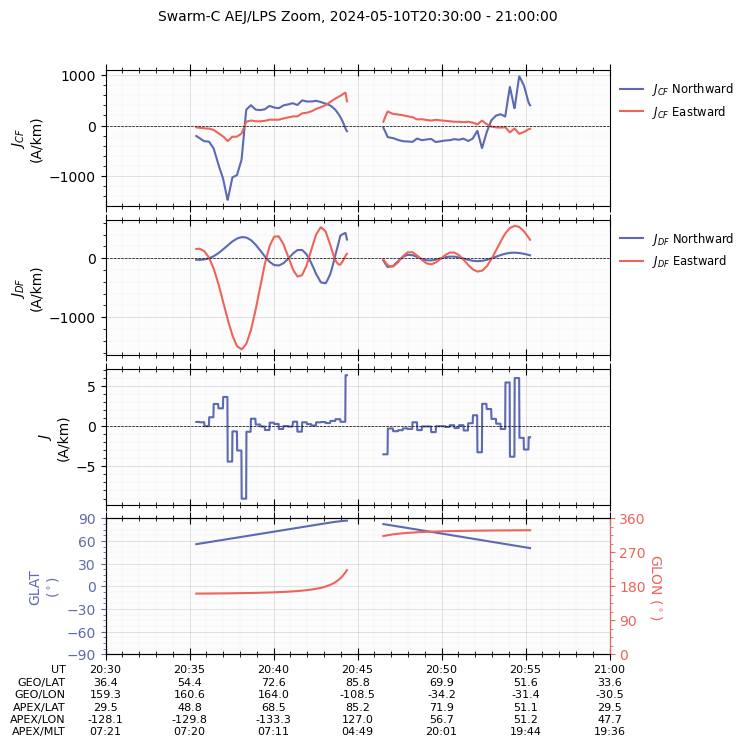
\includegraphics[width=0.7\linewidth]{files/317268c2a6e1aea8a2b62e50bc7510d4.png}

\paragraph{Swarm AEJ PBL data product}

\subparagraph{Overview with a long time span}

\begin{verbatim}
def test_swarm_AEJ_PBL_overview():
    """Test Swarm AEJ/PBL data product
    
    """
    dt_fr = datetime.datetime(2024, 5, 10, 12, 0)
    dt_to = datetime.datetime(2024, 5, 11, 12, 0)

    db = dashboards.TSDashboard(
        dt_fr=dt_fr, dt_to=dt_to, figure_config={'figsize': (8, 8)},
        )

    ds = db.dock(datasource_contents=['esa_eo', 'swarm', 'l2daily', 'aej_pbl'], sat_id='C', add_APEX=True, add_AACGM=True)

    panel_layouts = [
        [ds['WEJ_PEAK'], ds['EEJ_PEAK']],
        [
            ds['GEO_LAT_WEJ_PB'],
            ds['GEO_LAT_WEJ_PEAK'], 
            ds['GEO_LAT_WEJ_EB'],
            ds['GEO_LAT_EEJ_PB'],
            ds['GEO_LAT_EEJ_PEAK'],
            ds['GEO_LAT_EEJ_EB'],
        ],
        [
            ds['QD_LAT_WEJ_PB'],
            ds['QD_LAT_WEJ_PEAK'],
            ds['QD_LAT_WEJ_EB'],
            ds['QD_LAT_EEJ_PB'],
            ds['QD_LAT_EEJ_PEAK'],
            ds['QD_LAT_EEJ_EB'],
        ],
        [
            ds['QUALITY_FLAG_BIN_AUX'],
        ],
    ]

    db.set_layout(panel_layouts=panel_layouts)
    db.draw()
    db.add_title(title='Swarm -{} AEJ/PBL Overview'.format(ds.sat_id), fontsize='medium', append_time=True)

    db.show()
test_swarm_AEJ_PBL_overview()
\end{verbatim}

\begin{verbatim}
Create a new figure: Figure(800x800).
Searching the data product "AEJ_PBL" with the version "latest" on the server...
INFO: Indexing the files for the product AEJ_PBL of the satellite C ...
The file [PosixPath('/data/afys -ionosphere/data/ESA/SWARM/Level2daily/AEJ_PBL/0301/Sat_C/2024/SW_OPER_AEJCPBL_2F_20240101T000000_20241231T235959_0301.cdf')] already exists: skip downloading.
/opt/anaconda3/envs/Swarm/lib/python3.12/site -packages/apexpy/apex.py:556: RuntimeWarning: invalid value encountered in <lambda> (vectorized)
  alat, alon = self._geo2apex(glat, glon, height)
/opt/anaconda3/envs/Swarm/lib/python3.12/site -packages/apexpy/apex.py:559: UserWarning: Apex latitude set to NaN where undefined (apex height may be < reference height)
  warnings.warn(''.join(['Apex latitude set to NaN where undefined ',
/opt/anaconda3/envs/Swarm/lib/python3.12/site -packages/apexpy/apex.py:559: UserWarning: Apex latitude set to NaN where undefined (apex height may be < reference height)
  warnings.warn(''.join(['Apex latitude set to NaN where undefined ',
/opt/anaconda3/envs/Swarm/lib/python3.12/site -packages/apexpy/apex.py:559: UserWarning: Apex latitude set to NaN where undefined (apex height may be < reference height)
  warnings.warn(''.join(['Apex latitude set to NaN where undefined ',
/opt/anaconda3/envs/Swarm/lib/python3.12/site -packages/apexpy/apex.py:559: UserWarning: Apex latitude set to NaN where undefined (apex height may be < reference height)
  warnings.warn(''.join(['Apex latitude set to NaN where undefined ',
/opt/anaconda3/envs/Swarm/lib/python3.12/site -packages/apexpy/apex.py:559: UserWarning: Apex latitude set to NaN where undefined (apex height may be < reference height)
  warnings.warn(''.join(['Apex latitude set to NaN where undefined ',
/opt/anaconda3/envs/Swarm/lib/python3.12/site -packages/apexpy/apex.py:559: UserWarning: Apex latitude set to NaN where undefined (apex height may be < reference height)
  warnings.warn(''.join(['Apex latitude set to NaN where undefined ',
/opt/anaconda3/envs/Swarm/lib/python3.12/site -packages/apexpy/apex.py:559: UserWarning: Apex latitude set to NaN where undefined (apex height may be < reference height)
  warnings.warn(''.join(['Apex latitude set to NaN where undefined ',
/opt/anaconda3/envs/Swarm/lib/python3.12/site -packages/apexpy/apex.py:559: UserWarning: Apex latitude set to NaN where undefined (apex height may be < reference height)
  warnings.warn(''.join(['Apex latitude set to NaN where undefined ',
/opt/anaconda3/envs/Swarm/lib/python3.12/site -packages/apexpy/apex.py:559: UserWarning: Apex latitude set to NaN where undefined (apex height may be < reference height)
  warnings.warn(''.join(['Apex latitude set to NaN where undefined ',
/opt/anaconda3/envs/Swarm/lib/python3.12/site -packages/apexpy/apex.py:559: UserWarning: Apex latitude set to NaN where undefined (apex height may be < reference height)
  warnings.warn(''.join(['Apex latitude set to NaN where undefined ',
/opt/anaconda3/envs/Swarm/lib/python3.12/site -packages/apexpy/apex.py:559: UserWarning: Apex latitude set to NaN where undefined (apex height may be < reference height)
  warnings.warn(''.join(['Apex latitude set to NaN where undefined ',
/opt/anaconda3/envs/Swarm/lib/python3.12/site -packages/apexpy/apex.py:559: UserWarning: Apex latitude set to NaN where undefined (apex height may be < reference height)
  warnings.warn(''.join(['Apex latitude set to NaN where undefined ',
\end{verbatim}

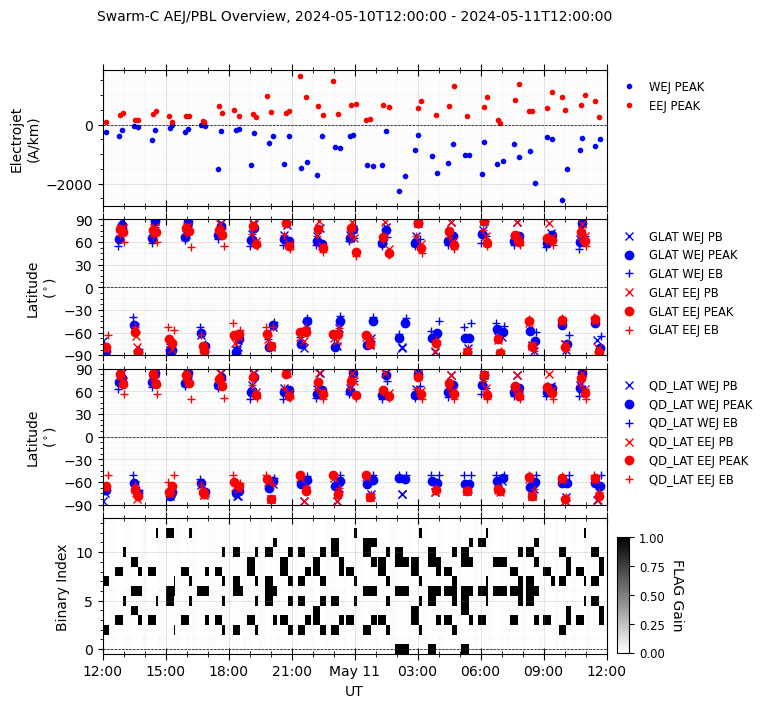
\includegraphics[width=0.7\linewidth]{files/72f8bfc9edf3f1fcc246fd249b049a13.png}

\subparagraph{Zoomed-in view with a short time span}

\begin{verbatim}
def test_swarm_AEJ_PBL_zoom():
    """Test Swarm AEJ/PBL data product
    
    """
    dt_fr = datetime.datetime(2024, 5, 10, 20, 30)
    dt_to = datetime.datetime(2024, 5, 10, 21, 0)

    db = dashboards.TSDashboard(
        dt_fr=dt_fr, dt_to=dt_to, figure_config={'figsize': (8, 8)},
        # timeline_extra_labels=['GEO_LAT', 'GEO_LON', 'APEX_LAT', 'APEX_LON', 'APEX_MLT',]  # Not applicable for very scattered data points like AEJ_PBL peaks
        )

    ds = db.dock(datasource_contents=['esa_eo', 'swarm', 'l2daily', 'aej_pbl'], sat_id='C', add_APEX=True, add_AACGM=True)

    panel_layouts = [
        [ds['WEJ_PEAK'], ds['EEJ_PEAK']],
        [
            ds['GEO_LAT_WEJ_PB'],
            ds['GEO_LAT_WEJ_PEAK'], 
            ds['GEO_LAT_WEJ_EB'],
            ds['GEO_LAT_EEJ_PB'],
            ds['GEO_LAT_EEJ_PEAK'],
            ds['GEO_LAT_EEJ_EB'],
            ],
        [
            ds['QD_LAT_WEJ_PB'],
            ds['QD_LAT_WEJ_PEAK'],
            ds['QD_LAT_WEJ_EB'],
            ds['QD_LAT_EEJ_PB'],
            ds['QD_LAT_EEJ_PEAK'],
            ds['QD_LAT_EEJ_EB'],
            ],
        [
            ds['QUALITY_FLAG_BIN_AUX'],
        ],
    ]

    db.set_layout(panel_layouts=panel_layouts)
    db.draw()
    db.add_title(title='Swarm -{} AEJ/PBL Zoom'.format(ds.sat_id), fontsize='medium', append_time=True)
    
    db.show()
test_swarm_AEJ_PBL_zoom()
\end{verbatim}

\begin{verbatim}
Create a new figure: Figure(800x800).
Searching the data product "AEJ_PBL" with the version "latest" on the server...
The file [PosixPath('/data/afys -ionosphere/data/ESA/SWARM/Level2daily/AEJ_PBL/0301/Sat_C/2024/SW_OPER_AEJCPBL_2F_20240101T000000_20241231T235959_0301.cdf')] already exists: skip downloading.
\end{verbatim}

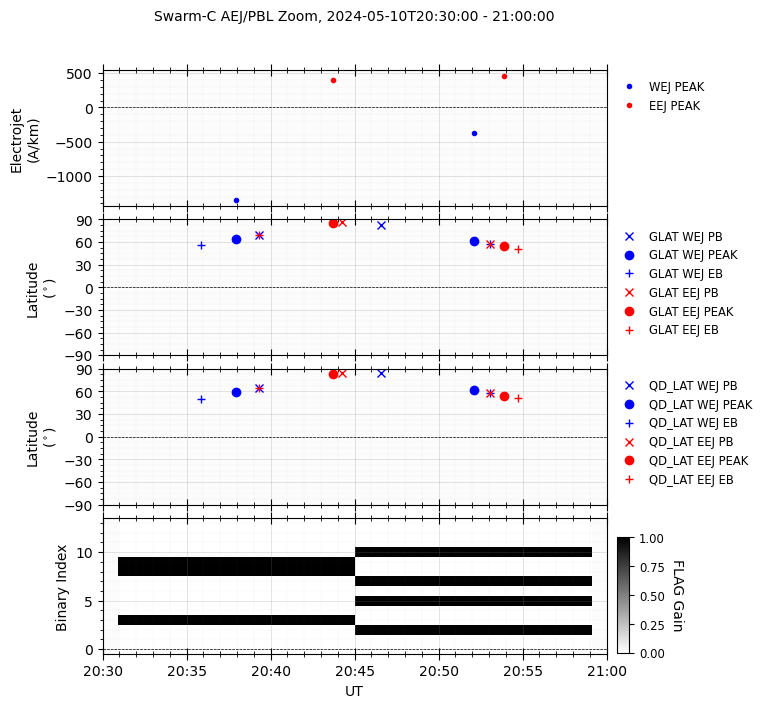
\includegraphics[width=0.7\linewidth]{files/eaf3f337786bc162074587a70df71bec.png}

\paragraph{Swarm AEJ PBS data product}

\subparagraph{Overview with a long time span}

\begin{verbatim}
def test_swarm_AEJ_PBS_overview():
    """Test Swarm AEJ/PBS data product
    
    """
    dt_fr = datetime.datetime(2024, 5, 10, 12, 0)
    dt_to = datetime.datetime(2024, 5, 11, 12, 0)

    db = dashboards.TSDashboard(
        dt_fr=dt_fr, dt_to=dt_to, figure_config={'figsize': (8, 8)},
        )

    ds = db.dock(datasource_contents=['esa_eo', 'swarm', 'l2daily', 'aej_pbs'], sat_id='C', add_APEX=True, add_AACGM=True)

    panel_layouts = [
        [ds['WEJ_PEAK'], ds['EEJ_PEAK']],
        [
            ds['GEO_LAT_WEJ_PB'],
            ds['GEO_LAT_WEJ_PEAK'], 
            ds['GEO_LAT_WEJ_EB'],
            ds['GEO_LAT_EEJ_PB'],
            ds['GEO_LAT_EEJ_PEAK'],
            ds['GEO_LAT_EEJ_EB'],
        ],
        [
            ds['QD_LAT_WEJ_PB'],
            ds['QD_LAT_WEJ_PEAK'],
            ds['QD_LAT_WEJ_EB'],
            ds['QD_LAT_EEJ_PB'],
            ds['QD_LAT_EEJ_PEAK'],
            ds['QD_LAT_EEJ_EB'],
        ],
        [
            ds['QUALITY_FLAG_BIN_AUX'],
        ],
    ]

    db.set_layout(panel_layouts=panel_layouts)
    db.draw()
    db.add_title(title='Swarm -{} AEJ/PBS Overview'.format(ds.sat_id), fontsize='medium', append_time=True)

    db.show()
test_swarm_AEJ_PBS_overview()
\end{verbatim}

\begin{verbatim}
Create a new figure: Figure(800x800).
Searching the data product "AEJ_PBS" with the version "latest" on the server...
INFO: Indexing the files for the product AEJ_PBS of the satellite C ...
The file [PosixPath('/data/afys -ionosphere/data/ESA/SWARM/Level2daily/AEJ_PBS/0101/Sat_C/2024/SW_OPER_AEJCPBS_2F_20240101T000000_20241031T235959_0101.cdf')] already exists: skip downloading.
/opt/anaconda3/envs/Swarm/lib/python3.12/site -packages/apexpy/apex.py:559: UserWarning: Apex latitude set to NaN where undefined (apex height may be < reference height)
  warnings.warn(''.join(['Apex latitude set to NaN where undefined ',
/opt/anaconda3/envs/Swarm/lib/python3.12/site -packages/apexpy/apex.py:559: UserWarning: Apex latitude set to NaN where undefined (apex height may be < reference height)
  warnings.warn(''.join(['Apex latitude set to NaN where undefined ',
/opt/anaconda3/envs/Swarm/lib/python3.12/site -packages/apexpy/apex.py:559: UserWarning: Apex latitude set to NaN where undefined (apex height may be < reference height)
  warnings.warn(''.join(['Apex latitude set to NaN where undefined ',
/opt/anaconda3/envs/Swarm/lib/python3.12/site -packages/apexpy/apex.py:559: UserWarning: Apex latitude set to NaN where undefined (apex height may be < reference height)
  warnings.warn(''.join(['Apex latitude set to NaN where undefined ',
/opt/anaconda3/envs/Swarm/lib/python3.12/site -packages/apexpy/apex.py:559: UserWarning: Apex latitude set to NaN where undefined (apex height may be < reference height)
  warnings.warn(''.join(['Apex latitude set to NaN where undefined ',
/opt/anaconda3/envs/Swarm/lib/python3.12/site -packages/apexpy/apex.py:559: UserWarning: Apex latitude set to NaN where undefined (apex height may be < reference height)
  warnings.warn(''.join(['Apex latitude set to NaN where undefined ',
/opt/anaconda3/envs/Swarm/lib/python3.12/site -packages/apexpy/apex.py:559: UserWarning: Apex latitude set to NaN where undefined (apex height may be < reference height)
  warnings.warn(''.join(['Apex latitude set to NaN where undefined ',
/opt/anaconda3/envs/Swarm/lib/python3.12/site -packages/apexpy/apex.py:559: UserWarning: Apex latitude set to NaN where undefined (apex height may be < reference height)
  warnings.warn(''.join(['Apex latitude set to NaN where undefined ',
/opt/anaconda3/envs/Swarm/lib/python3.12/site -packages/apexpy/apex.py:559: UserWarning: Apex latitude set to NaN where undefined (apex height may be < reference height)
  warnings.warn(''.join(['Apex latitude set to NaN where undefined ',
/opt/anaconda3/envs/Swarm/lib/python3.12/site -packages/apexpy/apex.py:559: UserWarning: Apex latitude set to NaN where undefined (apex height may be < reference height)
  warnings.warn(''.join(['Apex latitude set to NaN where undefined ',
/opt/anaconda3/envs/Swarm/lib/python3.12/site -packages/apexpy/apex.py:559: UserWarning: Apex latitude set to NaN where undefined (apex height may be < reference height)
  warnings.warn(''.join(['Apex latitude set to NaN where undefined ',
/opt/anaconda3/envs/Swarm/lib/python3.12/site -packages/apexpy/apex.py:559: UserWarning: Apex latitude set to NaN where undefined (apex height may be < reference height)
  warnings.warn(''.join(['Apex latitude set to NaN where undefined ',
/opt/anaconda3/envs/Swarm/lib/python3.12/site -packages/apexpy/apex.py:559: UserWarning: Apex latitude set to NaN where undefined (apex height may be < reference height)
  warnings.warn(''.join(['Apex latitude set to NaN where undefined ',
/opt/anaconda3/envs/Swarm/lib/python3.12/site -packages/apexpy/apex.py:559: UserWarning: Apex latitude set to NaN where undefined (apex height may be < reference height)
  warnings.warn(''.join(['Apex latitude set to NaN where undefined ',
/opt/anaconda3/envs/Swarm/lib/python3.12/site -packages/apexpy/apex.py:559: UserWarning: Apex latitude set to NaN where undefined (apex height may be < reference height)
  warnings.warn(''.join(['Apex latitude set to NaN where undefined ',
\end{verbatim}

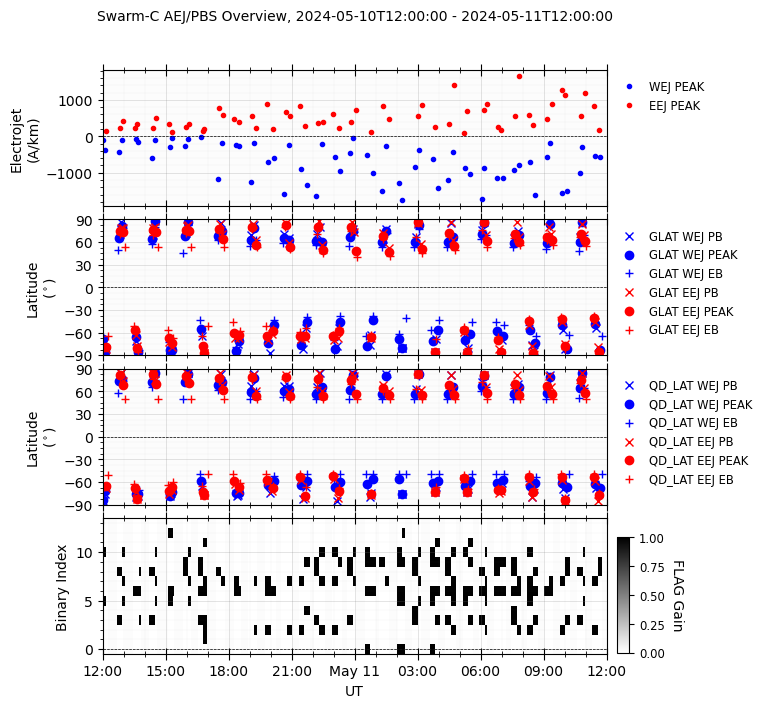
\includegraphics[width=0.7\linewidth]{files/6cd5ed9300edc4b0b9f53cad8e919269.png}

\subparagraph{Zoomed-in view with a short time span}

\begin{verbatim}
def test_swarm_AEJ_PBS_zoom():
    """Test Swarm AEJ/PBS data product
    
    """
    dt_fr = datetime.datetime(2024, 5, 10, 20, 30)
    dt_to = datetime.datetime(2024, 5, 10, 21, 0)

    db = dashboards.TSDashboard(
        dt_fr=dt_fr, dt_to=dt_to, figure_config={'figsize': (8, 8)},
        # timeline_extra_labels=['GEO_LAT', 'GEO_LON', 'APEX_LAT', 'APEX_LON', 'APEX_MLT',]  # Not applicable for very scattered data points like AEJ_PBS peaks
        )

    ds = db.dock(datasource_contents=['esa_eo', 'swarm', 'l2daily', 'aej_pbs'], sat_id='C', add_APEX=True, add_AACGM=True)

    panel_layouts = [
        [ds['WEJ_PEAK'], ds['EEJ_PEAK']],
        [
            ds['GEO_LAT_WEJ_PB'],
            ds['GEO_LAT_WEJ_PEAK'], 
            ds['GEO_LAT_WEJ_EB'],
            ds['GEO_LAT_EEJ_PB'],
            ds['GEO_LAT_EEJ_PEAK'],
            ds['GEO_LAT_EEJ_EB'],
            ],
        [
            ds['QD_LAT_WEJ_PB'],
            ds['QD_LAT_WEJ_PEAK'],
            ds['QD_LAT_WEJ_EB'],
            ds['QD_LAT_EEJ_PB'],
            ds['QD_LAT_EEJ_PEAK'],
            ds['QD_LAT_EEJ_EB'],
            ],
        [
            ds['QUALITY_FLAG_BIN_AUX'],
        ],
    ]

    db.set_layout(panel_layouts=panel_layouts)
    db.draw()
    db.add_title(title='Swarm -{} AEJ/PBS Zoom'.format(ds.sat_id), fontsize='medium', append_time=True)
    
    db.show()
test_swarm_AEJ_PBS_zoom()
\end{verbatim}

\begin{verbatim}
Create a new figure: Figure(800x800).
Searching the data product "AEJ_PBS" with the version "latest" on the server...
The file [PosixPath('/data/afys -ionosphere/data/ESA/SWARM/Level2daily/AEJ_PBS/0101/Sat_C/2024/SW_OPER_AEJCPBS_2F_20240101T000000_20241031T235959_0101.cdf')] already exists: skip downloading.
\end{verbatim}

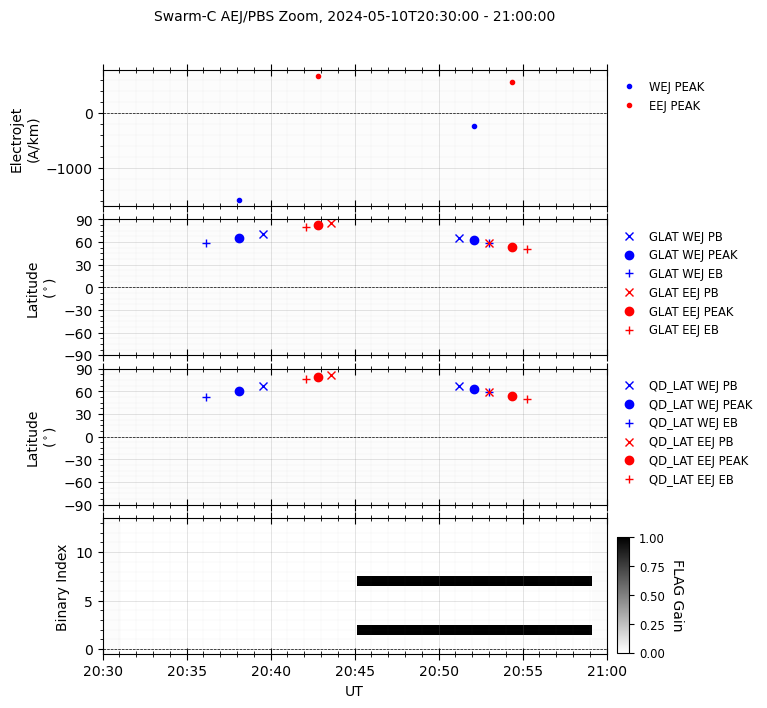
\includegraphics[width=0.7\linewidth]{files/2d6a3c8e43780af50e6393c403c30ad6.png}




\bibliography{main.bib}
\end{document}
